\documentclass[twoside]{book}

% Packages required by doxygen
\usepackage{fixltx2e}
\usepackage{calc}
\usepackage{doxygen}
\usepackage[export]{adjustbox} % also loads graphicx
\usepackage{graphicx}
\usepackage[utf8]{inputenc}
\usepackage{makeidx}
\usepackage{multicol}
\usepackage{multirow}
\PassOptionsToPackage{warn}{textcomp}
\usepackage{textcomp}
\usepackage[nointegrals]{wasysym}
\usepackage[table]{xcolor}

% Font selection
\usepackage[T1]{fontenc}
\usepackage[scaled=.90]{helvet}
\usepackage{courier}
\usepackage{amssymb}
\usepackage{sectsty}
\renewcommand{\familydefault}{\sfdefault}
\allsectionsfont{%
  \fontseries{bc}\selectfont%
  \color{darkgray}%
}
\renewcommand{\DoxyLabelFont}{%
  \fontseries{bc}\selectfont%
  \color{darkgray}%
}
\newcommand{\+}{\discretionary{\mbox{\scriptsize$\hookleftarrow$}}{}{}}

% Page & text layout
\usepackage{geometry}
\geometry{%
  a4paper,%
  top=2.5cm,%
  bottom=2.5cm,%
  left=2.5cm,%
  right=2.5cm%
}
\tolerance=750
\hfuzz=15pt
\hbadness=750
\setlength{\emergencystretch}{15pt}
\setlength{\parindent}{0cm}
\setlength{\parskip}{3ex plus 2ex minus 2ex}
\makeatletter
\renewcommand{\paragraph}{%
  \@startsection{paragraph}{4}{0ex}{-1.0ex}{1.0ex}{%
    \normalfont\normalsize\bfseries\SS@parafont%
  }%
}
\renewcommand{\subparagraph}{%
  \@startsection{subparagraph}{5}{0ex}{-1.0ex}{1.0ex}{%
    \normalfont\normalsize\bfseries\SS@subparafont%
  }%
}
\makeatother

% Headers & footers
\usepackage{fancyhdr}
\pagestyle{fancyplain}
\fancyhead[LE]{\fancyplain{}{\bfseries\thepage}}
\fancyhead[CE]{\fancyplain{}{}}
\fancyhead[RE]{\fancyplain{}{\bfseries\leftmark}}
\fancyhead[LO]{\fancyplain{}{\bfseries\rightmark}}
\fancyhead[CO]{\fancyplain{}{}}
\fancyhead[RO]{\fancyplain{}{\bfseries\thepage}}
\fancyfoot[LE]{\fancyplain{}{}}
\fancyfoot[CE]{\fancyplain{}{}}
\fancyfoot[RE]{\fancyplain{}{\bfseries\scriptsize Generated by Doxygen }}
\fancyfoot[LO]{\fancyplain{}{\bfseries\scriptsize Generated by Doxygen }}
\fancyfoot[CO]{\fancyplain{}{}}
\fancyfoot[RO]{\fancyplain{}{}}
\renewcommand{\footrulewidth}{0.4pt}
\renewcommand{\chaptermark}[1]{%
  \markboth{#1}{}%
}
\renewcommand{\sectionmark}[1]{%
  \markright{\thesection\ #1}%
}

% Indices & bibliography
\usepackage{natbib}
\usepackage[titles]{tocloft}
\setcounter{tocdepth}{3}
\setcounter{secnumdepth}{5}
\makeindex

% Hyperlinks (required, but should be loaded last)
\usepackage{ifpdf}
\ifpdf
  \usepackage[pdftex,pagebackref=true]{hyperref}
\else
  \usepackage[ps2pdf,pagebackref=true]{hyperref}
\fi
\hypersetup{%
  colorlinks=true,%
  linkcolor=blue,%
  citecolor=blue,%
  unicode%
}

% Custom commands
\newcommand{\clearemptydoublepage}{%
  \newpage{\pagestyle{empty}\cleardoublepage}%
}

\usepackage{caption}
\captionsetup{labelsep=space,justification=centering,font={bf},singlelinecheck=off,skip=4pt,position=top}

%===== C O N T E N T S =====

\begin{document}

% Titlepage & ToC
\hypersetup{pageanchor=false,
             bookmarksnumbered=true,
             pdfencoding=unicode
            }
\pagenumbering{roman}
\begin{titlepage}
\vspace*{7cm}
\begin{center}%
{\Large Week10 HW }\\
\vspace*{1cm}
{\large Generated by Doxygen 1.8.11}\\
\end{center}
\end{titlepage}
\clearemptydoublepage
\tableofcontents
\clearemptydoublepage
\pagenumbering{arabic}
\hypersetup{pageanchor=true}

%--- Begin generated contents ---
\chapter{Build procedures\+:}
\label{md_readme}
\hypertarget{md_readme}{}

\begin{DoxyEnumerate}
\item Create a catkin workspace using command catkin\+\_\+make in the workspace folder.
\item Make sure R\+O\+S\+\_\+\+P\+A\+C\+K\+A\+G\+E\+\_\+\+P\+A\+TH enviroment variable contain the workspace folder. This is done by sourcing the generated setup file under devel folder in the parent directory.
\item Create a package inside workspace src folder using command catkin\+\_\+create\+\_\+pkg beginning\+\_\+tutorials std\+\_\+msgs rospy roscpp.
\item Go back to parent directory and input command catkin\+\_\+make again.
\item Add talker and listener cpp files into the source folder under beginner\+\_\+tutorials package.
\item Modify Cmake\+Lists.\+txt to include talker and listener cpp files.
\item Include necessary dependencies like roscpp and std\+\_\+msgs and beginner\+\_\+tutorials\+\_\+generate\+\_\+messages\+\_\+cpp.
\end{DoxyEnumerate}

\subsection*{Run procedures\+:}


\begin{DoxyEnumerate}
\item Create three terminals. Make sure the package\textquotesingle{}s workspace is included in the P\+A\+TH variable.
\item Input roscore to establish a master.
\item Input 
\begin{DoxyCode}
1 rosrun beginner\_tutorials talker
\end{DoxyCode}
 in a different terminal to create the talker node.
\item Input 
\begin{DoxyCode}
1 rosrun beginner\_tutorials listener
\end{DoxyCode}
 in the final terminal to create the listener node. 
\end{DoxyEnumerate}
\chapter{Namespace Index}
\section{Namespace List}
Here is a list of all namespaces with brief descriptions\+:\begin{DoxyCompactList}
\item\contentsline{section}{\hyperlink{namespacecpplint}{cpplint} }{\pageref{namespacecpplint}}{}
\end{DoxyCompactList}

\chapter{Hierarchical Index}
\section{Class Hierarchy}
This inheritance list is sorted roughly, but not completely, alphabetically\+:\begin{DoxyCompactList}
\item Exception\begin{DoxyCompactList}
\item \contentsline{section}{cpplint.\+\_\+\+Include\+Error}{\pageref{classcpplint_1_1__IncludeError}}{}
\end{DoxyCompactList}
\item object\begin{DoxyCompactList}
\item \contentsline{section}{cpplint.\+\_\+\+Block\+Info}{\pageref{classcpplint_1_1__BlockInfo}}{}
\begin{DoxyCompactList}
\item \contentsline{section}{cpplint.\+\_\+\+Class\+Info}{\pageref{classcpplint_1_1__ClassInfo}}{}
\item \contentsline{section}{cpplint.\+\_\+\+Extern\+C\+Info}{\pageref{classcpplint_1_1__ExternCInfo}}{}
\item \contentsline{section}{cpplint.\+\_\+\+Namespace\+Info}{\pageref{classcpplint_1_1__NamespaceInfo}}{}
\end{DoxyCompactList}
\item \contentsline{section}{cpplint.\+\_\+\+Cpp\+Lint\+State}{\pageref{classcpplint_1_1__CppLintState}}{}
\item \contentsline{section}{cpplint.\+\_\+\+Function\+State}{\pageref{classcpplint_1_1__FunctionState}}{}
\item \contentsline{section}{cpplint.\+\_\+\+Include\+State}{\pageref{classcpplint_1_1__IncludeState}}{}
\item \contentsline{section}{cpplint.\+\_\+\+Preprocessor\+Info}{\pageref{classcpplint_1_1__PreprocessorInfo}}{}
\item \contentsline{section}{cpplint.\+Cleansed\+Lines}{\pageref{classcpplint_1_1CleansedLines}}{}
\item \contentsline{section}{cpplint.\+File\+Info}{\pageref{classcpplint_1_1FileInfo}}{}
\item \contentsline{section}{cpplint.\+Nesting\+State}{\pageref{classcpplint_1_1NestingState}}{}
\end{DoxyCompactList}
\end{DoxyCompactList}

\chapter{Class Index}
\section{Class List}
Here are the classes, structs, unions and interfaces with brief descriptions\+:\begin{DoxyCompactList}
\item\contentsline{section}{\hyperlink{classcpplint_1_1__BlockInfo}{cpplint.\+\_\+\+Block\+Info} }{\pageref{classcpplint_1_1__BlockInfo}}{}
\item\contentsline{section}{\hyperlink{classcpplint_1_1__ClassInfo}{cpplint.\+\_\+\+Class\+Info} }{\pageref{classcpplint_1_1__ClassInfo}}{}
\item\contentsline{section}{\hyperlink{classcpplint_1_1__CppLintState}{cpplint.\+\_\+\+Cpp\+Lint\+State} }{\pageref{classcpplint_1_1__CppLintState}}{}
\item\contentsline{section}{\hyperlink{classcpplint_1_1__ExternCInfo}{cpplint.\+\_\+\+Extern\+C\+Info} }{\pageref{classcpplint_1_1__ExternCInfo}}{}
\item\contentsline{section}{\hyperlink{classcpplint_1_1__FunctionState}{cpplint.\+\_\+\+Function\+State} }{\pageref{classcpplint_1_1__FunctionState}}{}
\item\contentsline{section}{\hyperlink{classcpplint_1_1__IncludeError}{cpplint.\+\_\+\+Include\+Error} }{\pageref{classcpplint_1_1__IncludeError}}{}
\item\contentsline{section}{\hyperlink{classcpplint_1_1__IncludeState}{cpplint.\+\_\+\+Include\+State} }{\pageref{classcpplint_1_1__IncludeState}}{}
\item\contentsline{section}{\hyperlink{classcpplint_1_1__NamespaceInfo}{cpplint.\+\_\+\+Namespace\+Info} }{\pageref{classcpplint_1_1__NamespaceInfo}}{}
\item\contentsline{section}{\hyperlink{classcpplint_1_1__PreprocessorInfo}{cpplint.\+\_\+\+Preprocessor\+Info} }{\pageref{classcpplint_1_1__PreprocessorInfo}}{}
\item\contentsline{section}{\hyperlink{classcpplint_1_1CleansedLines}{cpplint.\+Cleansed\+Lines} }{\pageref{classcpplint_1_1CleansedLines}}{}
\item\contentsline{section}{\hyperlink{classcpplint_1_1FileInfo}{cpplint.\+File\+Info} }{\pageref{classcpplint_1_1FileInfo}}{}
\item\contentsline{section}{\hyperlink{classcpplint_1_1NestingState}{cpplint.\+Nesting\+State} }{\pageref{classcpplint_1_1NestingState}}{}
\item\contentsline{section}{\hyperlink{classpassCustStr}{pass\+Cust\+Str} }{\pageref{classpassCustStr}}{}
\end{DoxyCompactList}

\chapter{File Index}
\section{File List}
Here is a list of all files with brief descriptions\+:\begin{DoxyCompactList}
\item\contentsline{section}{\hyperlink{cpplint_8py}{cpplint.\+py} }{\pageref{cpplint_8py}}{}
\item\contentsline{section}{include/\hyperlink{passCustStr_8hpp}{pass\+Cust\+Str.\+hpp} \\*This class is created to read and use the message received from the client. It contains a string and a bool function }{\pageref{passCustStr_8hpp}}{}
\item\contentsline{section}{src/\hyperlink{change__string__client_8cpp}{change\+\_\+string\+\_\+client.\+cpp} \\*This is the client node of the service \char`\"{}change\+\_\+string\char`\"{}. One would enter a string argument, which would be sent to the server node. And then, the server node would change its publishing content based on the string provided by the user. If no service is called, then the default string is \char`\"{}\+Hello\char`\"{} }{\pageref{change__string__client_8cpp}}{}
\item\contentsline{section}{src/\hyperlink{listener_8cpp}{listener.\+cpp} \\*Listener node within beginner\+\_\+tutorials package }{\pageref{listener_8cpp}}{}
\item\contentsline{section}{src/\hyperlink{passCustStr_8cpp}{pass\+Cust\+Str.\+cpp} }{\pageref{passCustStr_8cpp}}{}
\item\contentsline{section}{src/\hyperlink{talker_8cpp}{talker.\+cpp} \\*Talker noder within beginner\+\_\+tutorials package. It\textquotesingle{}s also a service node, a message publishing node, and a tf broadcasting node }{\pageref{talker_8cpp}}{}
\item\contentsline{section}{test/\hyperlink{talker__test_8cpp}{talker\+\_\+test.\+cpp} \\*Integration test on service/client nodes }{\pageref{talker__test_8cpp}}{}
\end{DoxyCompactList}

\chapter{Namespace Documentation}
\hypertarget{namespacecpplint}{}\section{cpplint Namespace Reference}
\label{namespacecpplint}\index{cpplint@{cpplint}}
\subsection*{Classes}
\begin{DoxyCompactItemize}
\item 
class \hyperlink{classcpplint_1_1__BlockInfo}{\+\_\+\+Block\+Info}
\item 
class \hyperlink{classcpplint_1_1__ClassInfo}{\+\_\+\+Class\+Info}
\item 
class \hyperlink{classcpplint_1_1__CppLintState}{\+\_\+\+Cpp\+Lint\+State}
\item 
class \hyperlink{classcpplint_1_1__ExternCInfo}{\+\_\+\+Extern\+C\+Info}
\item 
class \hyperlink{classcpplint_1_1__FunctionState}{\+\_\+\+Function\+State}
\item 
class \hyperlink{classcpplint_1_1__IncludeError}{\+\_\+\+Include\+Error}
\item 
class \hyperlink{classcpplint_1_1__IncludeState}{\+\_\+\+Include\+State}
\item 
class \hyperlink{classcpplint_1_1__NamespaceInfo}{\+\_\+\+Namespace\+Info}
\item 
class \hyperlink{classcpplint_1_1__PreprocessorInfo}{\+\_\+\+Preprocessor\+Info}
\item 
class \hyperlink{classcpplint_1_1CleansedLines}{Cleansed\+Lines}
\item 
class \hyperlink{classcpplint_1_1FileInfo}{File\+Info}
\item 
class \hyperlink{classcpplint_1_1NestingState}{Nesting\+State}
\end{DoxyCompactItemize}
\subsection*{Functions}
\begin{DoxyCompactItemize}
\item 
def \hyperlink{namespacecpplint_a28e546a8f20e32ef7dcf4ecbecd8b367}{Process\+Hpp\+Headers\+Option} (val)
\item 
def \hyperlink{namespacecpplint_ad4fd5ecbae967884b0a77ee8b3ba1e16}{Is\+Header\+Extension} (file\+\_\+extension)
\item 
def \hyperlink{namespacecpplint_a52ae8f1d9436d14ddb94ceed06026c43}{Parse\+Nolint\+Suppressions} (filename, raw\+\_\+line, linenum, error)
\item 
def \hyperlink{namespacecpplint_a316dc237dc0cde7bafec3c30d5624cac}{Process\+Global\+Suppresions} (lines)
\item 
def \hyperlink{namespacecpplint_a1d92dc3582da477f98ab5b85bd13fea0}{Reset\+Nolint\+Suppressions} ()
\item 
def \hyperlink{namespacecpplint_a0b9e1f991f1a3d02cda3234784241d1f}{Is\+Error\+Suppressed\+By\+Nolint} (category, linenum)
\item 
def \hyperlink{namespacecpplint_a73ac2ecfcd9c52b4a3755176c68dea7e}{Match} (pattern, s)
\item 
def \hyperlink{namespacecpplint_a1b85a5657aeab8b4a0ed85e06aed3576}{Replace\+All} (pattern, rep, s)
\item 
def \hyperlink{namespacecpplint_a75eae6bb88590e904f751502c8ee4bab}{Search} (pattern, s)
\item 
def \hyperlink{namespacecpplint_ae51e76d6d73b36b9e965d2ac9d21d7c2}{Error} (filename, linenum, category, confidence, message)
\item 
def \hyperlink{namespacecpplint_a034b93866a853c2e21577fb371a7fa9d}{Is\+Cpp\+String} (line)
\item 
def \hyperlink{namespacecpplint_a61b3f81ef467e7cb417d13e9051180fc}{Cleanse\+Raw\+Strings} (raw\+\_\+lines)
\item 
def \hyperlink{namespacecpplint_af0404401670283c9d4f948180e427401}{Find\+Next\+Multi\+Line\+Comment\+Start} (lines, lineix)
\item 
def \hyperlink{namespacecpplint_a4965d6f615333f43155d9e430471e228}{Find\+Next\+Multi\+Line\+Comment\+End} (lines, lineix)
\item 
def \hyperlink{namespacecpplint_a3a5f71cdc2e78491b4bedde8a0103679}{Remove\+Multi\+Line\+Comments\+From\+Range} (lines, begin, end)
\item 
def \hyperlink{namespacecpplint_ac259a6d0f292aeec05dee7ca312e1fc2}{Remove\+Multi\+Line\+Comments} (filename, lines, error)
\item 
def \hyperlink{namespacecpplint_ad795aa89f263838ec59fb0e7c52c842a}{Cleanse\+Comments} (line)
\item 
def \hyperlink{namespacecpplint_a6e623c46c1ae3bf650454744a693a633}{Find\+End\+Of\+Expression\+In\+Line} (line, startpos, stack)
\item 
def \hyperlink{namespacecpplint_af254258f584f59c87fcfd755e3c9017a}{Close\+Expression} (clean\+\_\+lines, linenum, pos)
\item 
def \hyperlink{namespacecpplint_a8572f47efb3bc11632d1192fd74bb7eb}{Find\+Start\+Of\+Expression\+In\+Line} (line, endpos, stack)
\item 
def \hyperlink{namespacecpplint_a15cd96cbf1c13e655e156fbd98cf0bae}{Reverse\+Close\+Expression} (clean\+\_\+lines, linenum, pos)
\item 
def \hyperlink{namespacecpplint_a0ad6bf921300c829db3696b81fa52d20}{Check\+For\+Copyright} (filename, lines, error)
\item 
def \hyperlink{namespacecpplint_a1b5cb7c1367845d7c7079eac5ea61dc8}{Get\+Indent\+Level} (line)
\item 
def \hyperlink{namespacecpplint_a3f143d4e8f70c0fd05e3f0ce81b0cc9a}{Get\+Header\+Guard\+C\+P\+P\+Variable} (filename)
\item 
def \hyperlink{namespacecpplint_a3694fa1b195f49a0d78dfc81ee665eec}{Check\+For\+Header\+Guard} (filename, clean\+\_\+lines, error)
\item 
def \hyperlink{namespacecpplint_ab549dcced7ca1d4b24538ec52b42439e}{Check\+Header\+File\+Included} (filename, include\+\_\+state, error)
\item 
def \hyperlink{namespacecpplint_a03c0e0d285b02b0e26ec514761654da8}{Check\+For\+Bad\+Characters} (filename, lines, error)
\item 
def \hyperlink{namespacecpplint_a7a594af230939932174dd5743088027d}{Check\+For\+Newline\+At\+E\+OF} (filename, lines, error)
\item 
def \hyperlink{namespacecpplint_a81c4baf76bde576f56661c22d01e470d}{Check\+For\+Multiline\+Comments\+And\+Strings} (filename, clean\+\_\+lines, linenum, error)
\item 
def \hyperlink{namespacecpplint_a9c406c00843a2c47058b1e9dec4e5b11}{Check\+Posix\+Threading} (filename, clean\+\_\+lines, linenum, error)
\item 
def \hyperlink{namespacecpplint_ab066834feaa7bf5a92982bbfb0af89c1}{Check\+Vlog\+Arguments} (filename, clean\+\_\+lines, linenum, error)
\item 
def \hyperlink{namespacecpplint_a8b47da46bc61f72ab12e9228acc3a0cd}{Check\+Invalid\+Increment} (filename, clean\+\_\+lines, linenum, error)
\item 
def \hyperlink{namespacecpplint_a5a95ee1e23638e172a3361723503329c}{Is\+Macro\+Definition} (clean\+\_\+lines, linenum)
\item 
def \hyperlink{namespacecpplint_adde7d60b6354b40d9ef9acda6e847d7b}{Is\+Forward\+Class\+Declaration} (clean\+\_\+lines, linenum)
\item 
def \hyperlink{namespacecpplint_a954b179c4037e5da8ac599cce095c37e}{Check\+For\+Non\+Standard\+Constructs} (filename, clean\+\_\+lines, linenum, nesting\+\_\+state, error)
\item 
def \hyperlink{namespacecpplint_a2ea8b2c917d5ce466287e1c6fe26f0db}{Check\+Spacing\+For\+Function\+Call} (filename, clean\+\_\+lines, linenum, error)
\item 
def \hyperlink{namespacecpplint_adf59429f3dd145e978624fe239809260}{Is\+Blank\+Line} (line)
\item 
def \hyperlink{namespacecpplint_a7c5964127d06521a2a05fbb28cc26478}{Check\+For\+Namespace\+Indentation} (filename, nesting\+\_\+state, clean\+\_\+lines, line, error)
\item 
def \hyperlink{namespacecpplint_a2699a7cad55a82cab5f73c012747203e}{Check\+For\+Function\+Lengths} (filename, clean\+\_\+lines, linenum, function\+\_\+state, error)
\item 
def \hyperlink{namespacecpplint_af126b85f4c25f359c40ce349f4eb7a2d}{Check\+Comment} (line, filename, linenum, next\+\_\+line\+\_\+start, error)
\item 
def \hyperlink{namespacecpplint_a73e82f51a8d59c816db26b5f797b3431}{Check\+Spacing} (filename, clean\+\_\+lines, linenum, nesting\+\_\+state, error)
\item 
def \hyperlink{namespacecpplint_a6a15b27f48cfd70fbf76f595c34f6d9e}{Check\+Operator\+Spacing} (filename, clean\+\_\+lines, linenum, error)
\item 
def \hyperlink{namespacecpplint_aacf5fa793ab27c7038e376d6a4c53d87}{Check\+Parenthesis\+Spacing} (filename, clean\+\_\+lines, linenum, error)
\item 
def \hyperlink{namespacecpplint_a46d2c48a2d4e747feee44616af987bdf}{Check\+Comma\+Spacing} (filename, clean\+\_\+lines, linenum, error)
\item 
def \hyperlink{namespacecpplint_a205bb76a59359eb1c0be86567bbc5256}{Check\+Braces\+Spacing} (filename, clean\+\_\+lines, linenum, nesting\+\_\+state, error)
\item 
def \hyperlink{namespacecpplint_a6e55ab13af2fa8b8e1f50e09aed592b8}{Is\+Decltype} (clean\+\_\+lines, linenum, column)
\item 
def \hyperlink{namespacecpplint_abc4e2f3f48debd6ae3a9561d052a955b}{Check\+Section\+Spacing} (filename, clean\+\_\+lines, class\+\_\+info, linenum, error)
\item 
def \hyperlink{namespacecpplint_a27743480b080a71eb8a0320da2ca0fa3}{Get\+Previous\+Non\+Blank\+Line} (clean\+\_\+lines, linenum)
\item 
def \hyperlink{namespacecpplint_a3f0a4d2ab1846bf487c742dc88946e3e}{Check\+Braces} (filename, clean\+\_\+lines, linenum, error)
\item 
def \hyperlink{namespacecpplint_a725663cb5a341fbf726f2ac8fa4e61a3}{Check\+Trailing\+Semicolon} (filename, clean\+\_\+lines, linenum, error)
\item 
def \hyperlink{namespacecpplint_a9c8aa68644d8cb55497a7d9cb8fb12d1}{Check\+Empty\+Block\+Body} (filename, clean\+\_\+lines, linenum, error)
\item 
def \hyperlink{namespacecpplint_aefff9c2eefe99656a226d11ce4d9b555}{Find\+Check\+Macro} (line)
\item 
def \hyperlink{namespacecpplint_afc5b544f640cd11be2665e6bb4646de7}{Check\+Check} (filename, clean\+\_\+lines, linenum, error)
\item 
def \hyperlink{namespacecpplint_a47f66a697e177c06b56491613fbc2d38}{Check\+Alt\+Tokens} (filename, clean\+\_\+lines, linenum, error)
\item 
def \hyperlink{namespacecpplint_ae55f74f34d41b59cf262511c5944209a}{Get\+Line\+Width} (line)
\item 
def \hyperlink{namespacecpplint_acfc546daa5947842cb01af319dcb482b}{Check\+Style} (filename, clean\+\_\+lines, linenum, file\+\_\+extension, nesting\+\_\+state, error)
\item 
def \hyperlink{namespacecpplint_add7eb8486a182205bb86de635db01384}{Check\+Include\+Line} (filename, clean\+\_\+lines, linenum, include\+\_\+state, error)
\item 
def \hyperlink{namespacecpplint_a6992d951cf4be06500f6b392ee6a8111}{Check\+Language} (filename, clean\+\_\+lines, linenum, file\+\_\+extension, include\+\_\+state, nesting\+\_\+state, error)
\item 
def \hyperlink{namespacecpplint_a64fc322bcf08988b43f003ff495fbabb}{Check\+Global\+Static} (filename, clean\+\_\+lines, linenum, error)
\item 
def \hyperlink{namespacecpplint_aaa8b988b9e83ad1c8964ecc0739d52e5}{Check\+Printf} (filename, clean\+\_\+lines, linenum, error)
\item 
def \hyperlink{namespacecpplint_ac8519cf084d818c931eac29994b03f55}{Is\+Derived\+Function} (clean\+\_\+lines, linenum)
\item 
def \hyperlink{namespacecpplint_a52e4468f674e140c256254eb0d1cf007}{Is\+Out\+Of\+Line\+Method\+Definition} (clean\+\_\+lines, linenum)
\item 
def \hyperlink{namespacecpplint_ae06fb1dd669681214573c0441b7e854f}{Is\+Initializer\+List} (clean\+\_\+lines, linenum)
\item 
def \hyperlink{namespacecpplint_a97f01c7d6e7e6d38b52744ab393d4160}{Check\+For\+Non\+Const\+Reference} (filename, clean\+\_\+lines, linenum, nesting\+\_\+state, error)
\item 
def \hyperlink{namespacecpplint_a59c5f44ae1dbedad109809d46e80588e}{Check\+Casts} (filename, clean\+\_\+lines, linenum, error)
\item 
def \hyperlink{namespacecpplint_ac23d9b29d869054db2ece1e7d5196349}{Check\+C\+Style\+Cast} (filename, clean\+\_\+lines, linenum, cast\+\_\+type, pattern, error)
\item 
def \hyperlink{namespacecpplint_a7657def0315cfe229ba436632f2d5042}{Expecting\+Function\+Args} (clean\+\_\+lines, linenum)
\item 
def \hyperlink{namespacecpplint_a66083e7d453e845a2751e76043fcd9ea}{Files\+Belong\+To\+Same\+Module} (filename\+\_\+cc, filename\+\_\+h)
\item 
def \hyperlink{namespacecpplint_a127416bee5c376937479b3119a727817}{Update\+Include\+State} (filename, include\+\_\+dict, io=codecs)
\item 
def \hyperlink{namespacecpplint_a8e1a5bea9f77246f8a0ae98a23d8d04e}{Check\+For\+Include\+What\+You\+Use} (filename, clean\+\_\+lines, include\+\_\+state, error, io=codecs)
\item 
def \hyperlink{namespacecpplint_add392d0ab0e8bcfeea6d02410229a0cc}{Check\+Make\+Pair\+Uses\+Deduction} (filename, clean\+\_\+lines, linenum, error)
\item 
def \hyperlink{namespacecpplint_a828985bee0575cfbb64212db74b61d9a}{Check\+Redundant\+Virtual} (filename, clean\+\_\+lines, linenum, error)
\item 
def \hyperlink{namespacecpplint_ab4f9b0390c702f149cec4030901d249d}{Check\+Redundant\+Override\+Or\+Final} (filename, clean\+\_\+lines, linenum, error)
\item 
def \hyperlink{namespacecpplint_a618e046738f246f01972bce339ee5d49}{Is\+Block\+In\+Name\+Space} (nesting\+\_\+state, is\+\_\+forward\+\_\+declaration)
\item 
def \hyperlink{namespacecpplint_aaaeb792789007d86b0898676c00caa72}{Should\+Check\+Namespace\+Indentation} (nesting\+\_\+state, is\+\_\+namespace\+\_\+indent\+\_\+item, raw\+\_\+lines\+\_\+no\+\_\+comments, linenum)
\item 
def \hyperlink{namespacecpplint_ac8e3b4340d0d83c8b2e7b199597b29a0}{Check\+Item\+Indentation\+In\+Namespace} (filename, raw\+\_\+lines\+\_\+no\+\_\+comments, linenum, error)
\item 
def \hyperlink{namespacecpplint_ac7c198c2adf60fd79a3f2b4270055a3b}{Process\+Line} (filename, file\+\_\+extension, clean\+\_\+lines, line, include\+\_\+state, function\+\_\+state, nesting\+\_\+state, error, extra\+\_\+check\+\_\+functions=\mbox{[}$\,$\mbox{]})
\item 
def \hyperlink{namespacecpplint_a386f43855367cc82348b0e2834e5cdc0}{Flag\+Cxx11\+Features} (filename, clean\+\_\+lines, linenum, error)
\item 
def \hyperlink{namespacecpplint_a744a4eecd461be0235779b03d34d6daf}{Flag\+Cxx14\+Features} (filename, clean\+\_\+lines, linenum, error)
\item 
def \hyperlink{namespacecpplint_ace3e46f0fab9638ad0e786037a5ca96c}{Process\+File\+Data} (filename, file\+\_\+extension, lines, error, extra\+\_\+check\+\_\+functions=\mbox{[}$\,$\mbox{]})
\item 
def \hyperlink{namespacecpplint_a6b67f01b8b199f5f6a7481fc0fb53878}{Process\+Config\+Overrides} (filename)
\item 
def \hyperlink{namespacecpplint_a41785091b61e8719f4a4a886eb20fe43}{Process\+File} (filename, vlevel, extra\+\_\+check\+\_\+functions=\mbox{[}$\,$\mbox{]})
\item 
def \hyperlink{namespacecpplint_a57542503fc1cce3e5c7171fc32d6ba05}{Print\+Usage} (message)
\item 
def \hyperlink{namespacecpplint_a3b1a047aa772a0d7d049d29c8ee62aba}{Print\+Categories} ()
\item 
def \hyperlink{namespacecpplint_a57476f6a7321d342db7b7ca98d80bd27}{Parse\+Arguments} (args)
\item 
def \hyperlink{namespacecpplint_a03dd39c6bfb4337676fcfaf5cd797c91}{main} ()
\end{DoxyCompactItemize}


\subsection{Function Documentation}
\index{cpplint@{cpplint}!Check\+Alt\+Tokens@{Check\+Alt\+Tokens}}
\index{Check\+Alt\+Tokens@{Check\+Alt\+Tokens}!cpplint@{cpplint}}
\subsubsection[{\texorpdfstring{Check\+Alt\+Tokens(filename, clean\+\_\+lines, linenum, error)}{CheckAltTokens(filename, clean_lines, linenum, error)}}]{\setlength{\rightskip}{0pt plus 5cm}def cpplint.\+Check\+Alt\+Tokens (
\begin{DoxyParamCaption}
\item[{}]{filename, }
\item[{}]{clean\+\_\+lines, }
\item[{}]{linenum, }
\item[{}]{error}
\end{DoxyParamCaption}
)}\hypertarget{namespacecpplint_a47f66a697e177c06b56491613fbc2d38}{}\label{namespacecpplint_a47f66a697e177c06b56491613fbc2d38}
\begin{DoxyVerb}Check alternative keywords being used in boolean expressions.

Args:
  filename: The name of the current file.
  clean_lines: A CleansedLines instance containing the file.
  linenum: The number of the line to check.
  error: The function to call with any errors found.
\end{DoxyVerb}
 \index{cpplint@{cpplint}!Check\+Braces@{Check\+Braces}}
\index{Check\+Braces@{Check\+Braces}!cpplint@{cpplint}}
\subsubsection[{\texorpdfstring{Check\+Braces(filename, clean\+\_\+lines, linenum, error)}{CheckBraces(filename, clean_lines, linenum, error)}}]{\setlength{\rightskip}{0pt plus 5cm}def cpplint.\+Check\+Braces (
\begin{DoxyParamCaption}
\item[{}]{filename, }
\item[{}]{clean\+\_\+lines, }
\item[{}]{linenum, }
\item[{}]{error}
\end{DoxyParamCaption}
)}\hypertarget{namespacecpplint_a3f0a4d2ab1846bf487c742dc88946e3e}{}\label{namespacecpplint_a3f0a4d2ab1846bf487c742dc88946e3e}
\begin{DoxyVerb}Looks for misplaced braces (e.g. at the end of line).

Args:
  filename: The name of the current file.
  clean_lines: A CleansedLines instance containing the file.
  linenum: The number of the line to check.
  error: The function to call with any errors found.
\end{DoxyVerb}
 \index{cpplint@{cpplint}!Check\+Braces\+Spacing@{Check\+Braces\+Spacing}}
\index{Check\+Braces\+Spacing@{Check\+Braces\+Spacing}!cpplint@{cpplint}}
\subsubsection[{\texorpdfstring{Check\+Braces\+Spacing(filename, clean\+\_\+lines, linenum, nesting\+\_\+state, error)}{CheckBracesSpacing(filename, clean_lines, linenum, nesting_state, error)}}]{\setlength{\rightskip}{0pt plus 5cm}def cpplint.\+Check\+Braces\+Spacing (
\begin{DoxyParamCaption}
\item[{}]{filename, }
\item[{}]{clean\+\_\+lines, }
\item[{}]{linenum, }
\item[{}]{nesting\+\_\+state, }
\item[{}]{error}
\end{DoxyParamCaption}
)}\hypertarget{namespacecpplint_a205bb76a59359eb1c0be86567bbc5256}{}\label{namespacecpplint_a205bb76a59359eb1c0be86567bbc5256}
\begin{DoxyVerb}Checks for horizontal spacing near commas.

Args:
  filename: The name of the current file.
  clean_lines: A CleansedLines instance containing the file.
  linenum: The number of the line to check.
  nesting_state: A NestingState instance which maintains information about
                 the current stack of nested blocks being parsed.
  error: The function to call with any errors found.
\end{DoxyVerb}
 \index{cpplint@{cpplint}!Check\+Casts@{Check\+Casts}}
\index{Check\+Casts@{Check\+Casts}!cpplint@{cpplint}}
\subsubsection[{\texorpdfstring{Check\+Casts(filename, clean\+\_\+lines, linenum, error)}{CheckCasts(filename, clean_lines, linenum, error)}}]{\setlength{\rightskip}{0pt plus 5cm}def cpplint.\+Check\+Casts (
\begin{DoxyParamCaption}
\item[{}]{filename, }
\item[{}]{clean\+\_\+lines, }
\item[{}]{linenum, }
\item[{}]{error}
\end{DoxyParamCaption}
)}\hypertarget{namespacecpplint_a59c5f44ae1dbedad109809d46e80588e}{}\label{namespacecpplint_a59c5f44ae1dbedad109809d46e80588e}
\begin{DoxyVerb}Various cast related checks.

Args:
  filename: The name of the current file.
  clean_lines: A CleansedLines instance containing the file.
  linenum: The number of the line to check.
  error: The function to call with any errors found.
\end{DoxyVerb}
 \index{cpplint@{cpplint}!Check\+Check@{Check\+Check}}
\index{Check\+Check@{Check\+Check}!cpplint@{cpplint}}
\subsubsection[{\texorpdfstring{Check\+Check(filename, clean\+\_\+lines, linenum, error)}{CheckCheck(filename, clean_lines, linenum, error)}}]{\setlength{\rightskip}{0pt plus 5cm}def cpplint.\+Check\+Check (
\begin{DoxyParamCaption}
\item[{}]{filename, }
\item[{}]{clean\+\_\+lines, }
\item[{}]{linenum, }
\item[{}]{error}
\end{DoxyParamCaption}
)}\hypertarget{namespacecpplint_afc5b544f640cd11be2665e6bb4646de7}{}\label{namespacecpplint_afc5b544f640cd11be2665e6bb4646de7}
\begin{DoxyVerb}Checks the use of CHECK and EXPECT macros.

Args:
  filename: The name of the current file.
  clean_lines: A CleansedLines instance containing the file.
  linenum: The number of the line to check.
  error: The function to call with any errors found.
\end{DoxyVerb}
 \index{cpplint@{cpplint}!Check\+Comma\+Spacing@{Check\+Comma\+Spacing}}
\index{Check\+Comma\+Spacing@{Check\+Comma\+Spacing}!cpplint@{cpplint}}
\subsubsection[{\texorpdfstring{Check\+Comma\+Spacing(filename, clean\+\_\+lines, linenum, error)}{CheckCommaSpacing(filename, clean_lines, linenum, error)}}]{\setlength{\rightskip}{0pt plus 5cm}def cpplint.\+Check\+Comma\+Spacing (
\begin{DoxyParamCaption}
\item[{}]{filename, }
\item[{}]{clean\+\_\+lines, }
\item[{}]{linenum, }
\item[{}]{error}
\end{DoxyParamCaption}
)}\hypertarget{namespacecpplint_a46d2c48a2d4e747feee44616af987bdf}{}\label{namespacecpplint_a46d2c48a2d4e747feee44616af987bdf}
\begin{DoxyVerb}Checks for horizontal spacing near commas and semicolons.

Args:
  filename: The name of the current file.
  clean_lines: A CleansedLines instance containing the file.
  linenum: The number of the line to check.
  error: The function to call with any errors found.
\end{DoxyVerb}
 \index{cpplint@{cpplint}!Check\+Comment@{Check\+Comment}}
\index{Check\+Comment@{Check\+Comment}!cpplint@{cpplint}}
\subsubsection[{\texorpdfstring{Check\+Comment(line, filename, linenum, next\+\_\+line\+\_\+start, error)}{CheckComment(line, filename, linenum, next_line_start, error)}}]{\setlength{\rightskip}{0pt plus 5cm}def cpplint.\+Check\+Comment (
\begin{DoxyParamCaption}
\item[{}]{line, }
\item[{}]{filename, }
\item[{}]{linenum, }
\item[{}]{next\+\_\+line\+\_\+start, }
\item[{}]{error}
\end{DoxyParamCaption}
)}\hypertarget{namespacecpplint_af126b85f4c25f359c40ce349f4eb7a2d}{}\label{namespacecpplint_af126b85f4c25f359c40ce349f4eb7a2d}
\begin{DoxyVerb}Checks for common mistakes in comments.

Args:
  line: The line in question.
  filename: The name of the current file.
  linenum: The number of the line to check.
  next_line_start: The first non-whitespace column of the next line.
  error: The function to call with any errors found.
\end{DoxyVerb}
 \index{cpplint@{cpplint}!Check\+C\+Style\+Cast@{Check\+C\+Style\+Cast}}
\index{Check\+C\+Style\+Cast@{Check\+C\+Style\+Cast}!cpplint@{cpplint}}
\subsubsection[{\texorpdfstring{Check\+C\+Style\+Cast(filename, clean\+\_\+lines, linenum, cast\+\_\+type, pattern, error)}{CheckCStyleCast(filename, clean_lines, linenum, cast_type, pattern, error)}}]{\setlength{\rightskip}{0pt plus 5cm}def cpplint.\+Check\+C\+Style\+Cast (
\begin{DoxyParamCaption}
\item[{}]{filename, }
\item[{}]{clean\+\_\+lines, }
\item[{}]{linenum, }
\item[{}]{cast\+\_\+type, }
\item[{}]{pattern, }
\item[{}]{error}
\end{DoxyParamCaption}
)}\hypertarget{namespacecpplint_ac23d9b29d869054db2ece1e7d5196349}{}\label{namespacecpplint_ac23d9b29d869054db2ece1e7d5196349}
\begin{DoxyVerb}Checks for a C-style cast by looking for the pattern.

Args:
  filename: The name of the current file.
  clean_lines: A CleansedLines instance containing the file.
  linenum: The number of the line to check.
  cast_type: The string for the C++ cast to recommend.  This is either
    reinterpret_cast, static_cast, or const_cast, depending.
  pattern: The regular expression used to find C-style casts.
  error: The function to call with any errors found.

Returns:
  True if an error was emitted.
  False otherwise.
\end{DoxyVerb}
 \index{cpplint@{cpplint}!Check\+Empty\+Block\+Body@{Check\+Empty\+Block\+Body}}
\index{Check\+Empty\+Block\+Body@{Check\+Empty\+Block\+Body}!cpplint@{cpplint}}
\subsubsection[{\texorpdfstring{Check\+Empty\+Block\+Body(filename, clean\+\_\+lines, linenum, error)}{CheckEmptyBlockBody(filename, clean_lines, linenum, error)}}]{\setlength{\rightskip}{0pt plus 5cm}def cpplint.\+Check\+Empty\+Block\+Body (
\begin{DoxyParamCaption}
\item[{}]{filename, }
\item[{}]{clean\+\_\+lines, }
\item[{}]{linenum, }
\item[{}]{error}
\end{DoxyParamCaption}
)}\hypertarget{namespacecpplint_a9c8aa68644d8cb55497a7d9cb8fb12d1}{}\label{namespacecpplint_a9c8aa68644d8cb55497a7d9cb8fb12d1}
\begin{DoxyVerb}Look for empty loop/conditional body with only a single semicolon.

Args:
  filename: The name of the current file.
  clean_lines: A CleansedLines instance containing the file.
  linenum: The number of the line to check.
  error: The function to call with any errors found.
\end{DoxyVerb}
 \index{cpplint@{cpplint}!Check\+For\+Bad\+Characters@{Check\+For\+Bad\+Characters}}
\index{Check\+For\+Bad\+Characters@{Check\+For\+Bad\+Characters}!cpplint@{cpplint}}
\subsubsection[{\texorpdfstring{Check\+For\+Bad\+Characters(filename, lines, error)}{CheckForBadCharacters(filename, lines, error)}}]{\setlength{\rightskip}{0pt plus 5cm}def cpplint.\+Check\+For\+Bad\+Characters (
\begin{DoxyParamCaption}
\item[{}]{filename, }
\item[{}]{lines, }
\item[{}]{error}
\end{DoxyParamCaption}
)}\hypertarget{namespacecpplint_a03c0e0d285b02b0e26ec514761654da8}{}\label{namespacecpplint_a03c0e0d285b02b0e26ec514761654da8}
\begin{DoxyVerb}Logs an error for each line containing bad characters.

Two kinds of bad characters:

1. Unicode replacement characters: These indicate that either the file
contained invalid UTF-8 (likely) or Unicode replacement characters (which
it shouldn't).  Note that it's possible for this to throw off line
numbering if the invalid UTF-8 occurred adjacent to a newline.

2. NUL bytes.  These are problematic for some tools.

Args:
  filename: The name of the current file.
  lines: An array of strings, each representing a line of the file.
  error: The function to call with any errors found.
\end{DoxyVerb}
 \index{cpplint@{cpplint}!Check\+For\+Copyright@{Check\+For\+Copyright}}
\index{Check\+For\+Copyright@{Check\+For\+Copyright}!cpplint@{cpplint}}
\subsubsection[{\texorpdfstring{Check\+For\+Copyright(filename, lines, error)}{CheckForCopyright(filename, lines, error)}}]{\setlength{\rightskip}{0pt plus 5cm}def cpplint.\+Check\+For\+Copyright (
\begin{DoxyParamCaption}
\item[{}]{filename, }
\item[{}]{lines, }
\item[{}]{error}
\end{DoxyParamCaption}
)}\hypertarget{namespacecpplint_a0ad6bf921300c829db3696b81fa52d20}{}\label{namespacecpplint_a0ad6bf921300c829db3696b81fa52d20}
\begin{DoxyVerb}Logs an error if no Copyright message appears at the top of the file.\end{DoxyVerb}
 \index{cpplint@{cpplint}!Check\+For\+Function\+Lengths@{Check\+For\+Function\+Lengths}}
\index{Check\+For\+Function\+Lengths@{Check\+For\+Function\+Lengths}!cpplint@{cpplint}}
\subsubsection[{\texorpdfstring{Check\+For\+Function\+Lengths(filename, clean\+\_\+lines, linenum, function\+\_\+state, error)}{CheckForFunctionLengths(filename, clean_lines, linenum, function_state, error)}}]{\setlength{\rightskip}{0pt plus 5cm}def cpplint.\+Check\+For\+Function\+Lengths (
\begin{DoxyParamCaption}
\item[{}]{filename, }
\item[{}]{clean\+\_\+lines, }
\item[{}]{linenum, }
\item[{}]{function\+\_\+state, }
\item[{}]{error}
\end{DoxyParamCaption}
)}\hypertarget{namespacecpplint_a2699a7cad55a82cab5f73c012747203e}{}\label{namespacecpplint_a2699a7cad55a82cab5f73c012747203e}
\begin{DoxyVerb}Reports for long function bodies.

For an overview why this is done, see:
https://google-styleguide.googlecode.com/svn/trunk/cppguide.xml#Write_Short_Functions

Uses a simplistic algorithm assuming other style guidelines
(especially spacing) are followed.
Only checks unindented functions, so class members are unchecked.
Trivial bodies are unchecked, so constructors with huge initializer lists
may be missed.
Blank/comment lines are not counted so as to avoid encouraging the removal
of vertical space and comments just to get through a lint check.
NOLINT *on the last line of a function* disables this check.

Args:
  filename: The name of the current file.
  clean_lines: A CleansedLines instance containing the file.
  linenum: The number of the line to check.
  function_state: Current function name and lines in body so far.
  error: The function to call with any errors found.
\end{DoxyVerb}
 \index{cpplint@{cpplint}!Check\+For\+Header\+Guard@{Check\+For\+Header\+Guard}}
\index{Check\+For\+Header\+Guard@{Check\+For\+Header\+Guard}!cpplint@{cpplint}}
\subsubsection[{\texorpdfstring{Check\+For\+Header\+Guard(filename, clean\+\_\+lines, error)}{CheckForHeaderGuard(filename, clean_lines, error)}}]{\setlength{\rightskip}{0pt plus 5cm}def cpplint.\+Check\+For\+Header\+Guard (
\begin{DoxyParamCaption}
\item[{}]{filename, }
\item[{}]{clean\+\_\+lines, }
\item[{}]{error}
\end{DoxyParamCaption}
)}\hypertarget{namespacecpplint_a3694fa1b195f49a0d78dfc81ee665eec}{}\label{namespacecpplint_a3694fa1b195f49a0d78dfc81ee665eec}
\begin{DoxyVerb}Checks that the file contains a header guard.

Logs an error if no #ifndef header guard is present.  For other
headers, checks that the full pathname is used.

Args:
  filename: The name of the C++ header file.
  clean_lines: A CleansedLines instance containing the file.
  error: The function to call with any errors found.
\end{DoxyVerb}
 \index{cpplint@{cpplint}!Check\+For\+Include\+What\+You\+Use@{Check\+For\+Include\+What\+You\+Use}}
\index{Check\+For\+Include\+What\+You\+Use@{Check\+For\+Include\+What\+You\+Use}!cpplint@{cpplint}}
\subsubsection[{\texorpdfstring{Check\+For\+Include\+What\+You\+Use(filename, clean\+\_\+lines, include\+\_\+state, error, io=codecs)}{CheckForIncludeWhatYouUse(filename, clean_lines, include_state, error, io=codecs)}}]{\setlength{\rightskip}{0pt plus 5cm}def cpplint.\+Check\+For\+Include\+What\+You\+Use (
\begin{DoxyParamCaption}
\item[{}]{filename, }
\item[{}]{clean\+\_\+lines, }
\item[{}]{include\+\_\+state, }
\item[{}]{error, }
\item[{}]{io = {\ttfamily codecs}}
\end{DoxyParamCaption}
)}\hypertarget{namespacecpplint_a8e1a5bea9f77246f8a0ae98a23d8d04e}{}\label{namespacecpplint_a8e1a5bea9f77246f8a0ae98a23d8d04e}
\begin{DoxyVerb}Reports for missing stl includes.

This function will output warnings to make sure you are including the headers
necessary for the stl containers and functions that you use. We only give one
reason to include a header. For example, if you use both equal_to<> and
less<> in a .h file, only one (the latter in the file) of these will be
reported as a reason to include the <functional>.

Args:
  filename: The name of the current file.
  clean_lines: A CleansedLines instance containing the file.
  include_state: An _IncludeState instance.
  error: The function to call with any errors found.
  io: The IO factory to use to read the header file. Provided for unittest
      injection.
\end{DoxyVerb}
 \index{cpplint@{cpplint}!Check\+For\+Multiline\+Comments\+And\+Strings@{Check\+For\+Multiline\+Comments\+And\+Strings}}
\index{Check\+For\+Multiline\+Comments\+And\+Strings@{Check\+For\+Multiline\+Comments\+And\+Strings}!cpplint@{cpplint}}
\subsubsection[{\texorpdfstring{Check\+For\+Multiline\+Comments\+And\+Strings(filename, clean\+\_\+lines, linenum, error)}{CheckForMultilineCommentsAndStrings(filename, clean_lines, linenum, error)}}]{\setlength{\rightskip}{0pt plus 5cm}def cpplint.\+Check\+For\+Multiline\+Comments\+And\+Strings (
\begin{DoxyParamCaption}
\item[{}]{filename, }
\item[{}]{clean\+\_\+lines, }
\item[{}]{linenum, }
\item[{}]{error}
\end{DoxyParamCaption}
)}\hypertarget{namespacecpplint_a81c4baf76bde576f56661c22d01e470d}{}\label{namespacecpplint_a81c4baf76bde576f56661c22d01e470d}
\begin{DoxyVerb}Logs an error if we see /* ... */ or "..." that extend past one line.

/* ... */ comments are legit inside macros, for one line.
Otherwise, we prefer // comments, so it's ok to warn about the
other.  Likewise, it's ok for strings to extend across multiple
lines, as long as a line continuation character (backslash)
terminates each line. Although not currently prohibited by the C++
style guide, it's ugly and unnecessary. We don't do well with either
in this lint program, so we warn about both.

Args:
  filename: The name of the current file.
  clean_lines: A CleansedLines instance containing the file.
  linenum: The number of the line to check.
  error: The function to call with any errors found.
\end{DoxyVerb}
 \index{cpplint@{cpplint}!Check\+For\+Namespace\+Indentation@{Check\+For\+Namespace\+Indentation}}
\index{Check\+For\+Namespace\+Indentation@{Check\+For\+Namespace\+Indentation}!cpplint@{cpplint}}
\subsubsection[{\texorpdfstring{Check\+For\+Namespace\+Indentation(filename, nesting\+\_\+state, clean\+\_\+lines, line, error)}{CheckForNamespaceIndentation(filename, nesting_state, clean_lines, line, error)}}]{\setlength{\rightskip}{0pt plus 5cm}def cpplint.\+Check\+For\+Namespace\+Indentation (
\begin{DoxyParamCaption}
\item[{}]{filename, }
\item[{}]{nesting\+\_\+state, }
\item[{}]{clean\+\_\+lines, }
\item[{}]{line, }
\item[{}]{error}
\end{DoxyParamCaption}
)}\hypertarget{namespacecpplint_a7c5964127d06521a2a05fbb28cc26478}{}\label{namespacecpplint_a7c5964127d06521a2a05fbb28cc26478}
\index{cpplint@{cpplint}!Check\+For\+Newline\+At\+E\+OF@{Check\+For\+Newline\+At\+E\+OF}}
\index{Check\+For\+Newline\+At\+E\+OF@{Check\+For\+Newline\+At\+E\+OF}!cpplint@{cpplint}}
\subsubsection[{\texorpdfstring{Check\+For\+Newline\+At\+E\+O\+F(filename, lines, error)}{CheckForNewlineAtEOF(filename, lines, error)}}]{\setlength{\rightskip}{0pt plus 5cm}def cpplint.\+Check\+For\+Newline\+At\+E\+OF (
\begin{DoxyParamCaption}
\item[{}]{filename, }
\item[{}]{lines, }
\item[{}]{error}
\end{DoxyParamCaption}
)}\hypertarget{namespacecpplint_a7a594af230939932174dd5743088027d}{}\label{namespacecpplint_a7a594af230939932174dd5743088027d}
\begin{DoxyVerb}Logs an error if there is no newline char at the end of the file.

Args:
  filename: The name of the current file.
  lines: An array of strings, each representing a line of the file.
  error: The function to call with any errors found.
\end{DoxyVerb}
 \index{cpplint@{cpplint}!Check\+For\+Non\+Const\+Reference@{Check\+For\+Non\+Const\+Reference}}
\index{Check\+For\+Non\+Const\+Reference@{Check\+For\+Non\+Const\+Reference}!cpplint@{cpplint}}
\subsubsection[{\texorpdfstring{Check\+For\+Non\+Const\+Reference(filename, clean\+\_\+lines, linenum, nesting\+\_\+state, error)}{CheckForNonConstReference(filename, clean_lines, linenum, nesting_state, error)}}]{\setlength{\rightskip}{0pt plus 5cm}def cpplint.\+Check\+For\+Non\+Const\+Reference (
\begin{DoxyParamCaption}
\item[{}]{filename, }
\item[{}]{clean\+\_\+lines, }
\item[{}]{linenum, }
\item[{}]{nesting\+\_\+state, }
\item[{}]{error}
\end{DoxyParamCaption}
)}\hypertarget{namespacecpplint_a97f01c7d6e7e6d38b52744ab393d4160}{}\label{namespacecpplint_a97f01c7d6e7e6d38b52744ab393d4160}
\begin{DoxyVerb}Check for non-const references.

Separate from CheckLanguage since it scans backwards from current
line, instead of scanning forward.

Args:
  filename: The name of the current file.
  clean_lines: A CleansedLines instance containing the file.
  linenum: The number of the line to check.
  nesting_state: A NestingState instance which maintains information about
                 the current stack of nested blocks being parsed.
  error: The function to call with any errors found.
\end{DoxyVerb}
 \index{cpplint@{cpplint}!Check\+For\+Non\+Standard\+Constructs@{Check\+For\+Non\+Standard\+Constructs}}
\index{Check\+For\+Non\+Standard\+Constructs@{Check\+For\+Non\+Standard\+Constructs}!cpplint@{cpplint}}
\subsubsection[{\texorpdfstring{Check\+For\+Non\+Standard\+Constructs(filename, clean\+\_\+lines, linenum, nesting\+\_\+state, error)}{CheckForNonStandardConstructs(filename, clean_lines, linenum, nesting_state, error)}}]{\setlength{\rightskip}{0pt plus 5cm}def cpplint.\+Check\+For\+Non\+Standard\+Constructs (
\begin{DoxyParamCaption}
\item[{}]{filename, }
\item[{}]{clean\+\_\+lines, }
\item[{}]{linenum, }
\item[{}]{nesting\+\_\+state, }
\item[{}]{error}
\end{DoxyParamCaption}
)}\hypertarget{namespacecpplint_a954b179c4037e5da8ac599cce095c37e}{}\label{namespacecpplint_a954b179c4037e5da8ac599cce095c37e}
\index{cpplint@{cpplint}!Check\+Global\+Static@{Check\+Global\+Static}}
\index{Check\+Global\+Static@{Check\+Global\+Static}!cpplint@{cpplint}}
\subsubsection[{\texorpdfstring{Check\+Global\+Static(filename, clean\+\_\+lines, linenum, error)}{CheckGlobalStatic(filename, clean_lines, linenum, error)}}]{\setlength{\rightskip}{0pt plus 5cm}def cpplint.\+Check\+Global\+Static (
\begin{DoxyParamCaption}
\item[{}]{filename, }
\item[{}]{clean\+\_\+lines, }
\item[{}]{linenum, }
\item[{}]{error}
\end{DoxyParamCaption}
)}\hypertarget{namespacecpplint_a64fc322bcf08988b43f003ff495fbabb}{}\label{namespacecpplint_a64fc322bcf08988b43f003ff495fbabb}
\begin{DoxyVerb}Check for unsafe global or static objects.

Args:
  filename: The name of the current file.
  clean_lines: A CleansedLines instance containing the file.
  linenum: The number of the line to check.
  error: The function to call with any errors found.
\end{DoxyVerb}
 \index{cpplint@{cpplint}!Check\+Header\+File\+Included@{Check\+Header\+File\+Included}}
\index{Check\+Header\+File\+Included@{Check\+Header\+File\+Included}!cpplint@{cpplint}}
\subsubsection[{\texorpdfstring{Check\+Header\+File\+Included(filename, include\+\_\+state, error)}{CheckHeaderFileIncluded(filename, include_state, error)}}]{\setlength{\rightskip}{0pt plus 5cm}def cpplint.\+Check\+Header\+File\+Included (
\begin{DoxyParamCaption}
\item[{}]{filename, }
\item[{}]{include\+\_\+state, }
\item[{}]{error}
\end{DoxyParamCaption}
)}\hypertarget{namespacecpplint_ab549dcced7ca1d4b24538ec52b42439e}{}\label{namespacecpplint_ab549dcced7ca1d4b24538ec52b42439e}
\begin{DoxyVerb}Logs an error if a .cc file does not include its header.\end{DoxyVerb}
 \index{cpplint@{cpplint}!Check\+Include\+Line@{Check\+Include\+Line}}
\index{Check\+Include\+Line@{Check\+Include\+Line}!cpplint@{cpplint}}
\subsubsection[{\texorpdfstring{Check\+Include\+Line(filename, clean\+\_\+lines, linenum, include\+\_\+state, error)}{CheckIncludeLine(filename, clean_lines, linenum, include_state, error)}}]{\setlength{\rightskip}{0pt plus 5cm}def cpplint.\+Check\+Include\+Line (
\begin{DoxyParamCaption}
\item[{}]{filename, }
\item[{}]{clean\+\_\+lines, }
\item[{}]{linenum, }
\item[{}]{include\+\_\+state, }
\item[{}]{error}
\end{DoxyParamCaption}
)}\hypertarget{namespacecpplint_add7eb8486a182205bb86de635db01384}{}\label{namespacecpplint_add7eb8486a182205bb86de635db01384}
\begin{DoxyVerb}Check rules that are applicable to #include lines.

Strings on #include lines are NOT removed from elided line, to make
certain tasks easier. However, to prevent false positives, checks
applicable to #include lines in CheckLanguage must be put here.

Args:
  filename: The name of the current file.
  clean_lines: A CleansedLines instance containing the file.
  linenum: The number of the line to check.
  include_state: An _IncludeState instance in which the headers are inserted.
  error: The function to call with any errors found.
\end{DoxyVerb}
 \index{cpplint@{cpplint}!Check\+Invalid\+Increment@{Check\+Invalid\+Increment}}
\index{Check\+Invalid\+Increment@{Check\+Invalid\+Increment}!cpplint@{cpplint}}
\subsubsection[{\texorpdfstring{Check\+Invalid\+Increment(filename, clean\+\_\+lines, linenum, error)}{CheckInvalidIncrement(filename, clean_lines, linenum, error)}}]{\setlength{\rightskip}{0pt plus 5cm}def cpplint.\+Check\+Invalid\+Increment (
\begin{DoxyParamCaption}
\item[{}]{filename, }
\item[{}]{clean\+\_\+lines, }
\item[{}]{linenum, }
\item[{}]{error}
\end{DoxyParamCaption}
)}\hypertarget{namespacecpplint_a8b47da46bc61f72ab12e9228acc3a0cd}{}\label{namespacecpplint_a8b47da46bc61f72ab12e9228acc3a0cd}
\begin{DoxyVerb}Checks for invalid increment *count++.

For example following function:
void increment_counter(int* count) {
  *count++;
}
is invalid, because it effectively does count++, moving pointer, and should
be replaced with ++*count, (*count)++ or *count += 1.

Args:
  filename: The name of the current file.
  clean_lines: A CleansedLines instance containing the file.
  linenum: The number of the line to check.
  error: The function to call with any errors found.
\end{DoxyVerb}
 \index{cpplint@{cpplint}!Check\+Item\+Indentation\+In\+Namespace@{Check\+Item\+Indentation\+In\+Namespace}}
\index{Check\+Item\+Indentation\+In\+Namespace@{Check\+Item\+Indentation\+In\+Namespace}!cpplint@{cpplint}}
\subsubsection[{\texorpdfstring{Check\+Item\+Indentation\+In\+Namespace(filename, raw\+\_\+lines\+\_\+no\+\_\+comments, linenum, error)}{CheckItemIndentationInNamespace(filename, raw_lines_no_comments, linenum, error)}}]{\setlength{\rightskip}{0pt plus 5cm}def cpplint.\+Check\+Item\+Indentation\+In\+Namespace (
\begin{DoxyParamCaption}
\item[{}]{filename, }
\item[{}]{raw\+\_\+lines\+\_\+no\+\_\+comments, }
\item[{}]{linenum, }
\item[{}]{error}
\end{DoxyParamCaption}
)}\hypertarget{namespacecpplint_ac8e3b4340d0d83c8b2e7b199597b29a0}{}\label{namespacecpplint_ac8e3b4340d0d83c8b2e7b199597b29a0}
\index{cpplint@{cpplint}!Check\+Language@{Check\+Language}}
\index{Check\+Language@{Check\+Language}!cpplint@{cpplint}}
\subsubsection[{\texorpdfstring{Check\+Language(filename, clean\+\_\+lines, linenum, file\+\_\+extension, include\+\_\+state, nesting\+\_\+state, error)}{CheckLanguage(filename, clean_lines, linenum, file_extension, include_state, nesting_state, error)}}]{\setlength{\rightskip}{0pt plus 5cm}def cpplint.\+Check\+Language (
\begin{DoxyParamCaption}
\item[{}]{filename, }
\item[{}]{clean\+\_\+lines, }
\item[{}]{linenum, }
\item[{}]{file\+\_\+extension, }
\item[{}]{include\+\_\+state, }
\item[{}]{nesting\+\_\+state, }
\item[{}]{error}
\end{DoxyParamCaption}
)}\hypertarget{namespacecpplint_a6992d951cf4be06500f6b392ee6a8111}{}\label{namespacecpplint_a6992d951cf4be06500f6b392ee6a8111}
\begin{DoxyVerb}Checks rules from the 'C++ language rules' section of cppguide.html.

Some of these rules are hard to test (function overloading, using
uint32 inappropriately), but we do the best we can.

Args:
  filename: The name of the current file.
  clean_lines: A CleansedLines instance containing the file.
  linenum: The number of the line to check.
  file_extension: The extension (without the dot) of the filename.
  include_state: An _IncludeState instance in which the headers are inserted.
  nesting_state: A NestingState instance which maintains information about
                 the current stack of nested blocks being parsed.
  error: The function to call with any errors found.
\end{DoxyVerb}
 \index{cpplint@{cpplint}!Check\+Make\+Pair\+Uses\+Deduction@{Check\+Make\+Pair\+Uses\+Deduction}}
\index{Check\+Make\+Pair\+Uses\+Deduction@{Check\+Make\+Pair\+Uses\+Deduction}!cpplint@{cpplint}}
\subsubsection[{\texorpdfstring{Check\+Make\+Pair\+Uses\+Deduction(filename, clean\+\_\+lines, linenum, error)}{CheckMakePairUsesDeduction(filename, clean_lines, linenum, error)}}]{\setlength{\rightskip}{0pt plus 5cm}def cpplint.\+Check\+Make\+Pair\+Uses\+Deduction (
\begin{DoxyParamCaption}
\item[{}]{filename, }
\item[{}]{clean\+\_\+lines, }
\item[{}]{linenum, }
\item[{}]{error}
\end{DoxyParamCaption}
)}\hypertarget{namespacecpplint_add392d0ab0e8bcfeea6d02410229a0cc}{}\label{namespacecpplint_add392d0ab0e8bcfeea6d02410229a0cc}
\begin{DoxyVerb}Check that make_pair's template arguments are deduced.

G++ 4.6 in C++11 mode fails badly if make_pair's template arguments are
specified explicitly, and such use isn't intended in any case.

Args:
  filename: The name of the current file.
  clean_lines: A CleansedLines instance containing the file.
  linenum: The number of the line to check.
  error: The function to call with any errors found.
\end{DoxyVerb}
 \index{cpplint@{cpplint}!Check\+Operator\+Spacing@{Check\+Operator\+Spacing}}
\index{Check\+Operator\+Spacing@{Check\+Operator\+Spacing}!cpplint@{cpplint}}
\subsubsection[{\texorpdfstring{Check\+Operator\+Spacing(filename, clean\+\_\+lines, linenum, error)}{CheckOperatorSpacing(filename, clean_lines, linenum, error)}}]{\setlength{\rightskip}{0pt plus 5cm}def cpplint.\+Check\+Operator\+Spacing (
\begin{DoxyParamCaption}
\item[{}]{filename, }
\item[{}]{clean\+\_\+lines, }
\item[{}]{linenum, }
\item[{}]{error}
\end{DoxyParamCaption}
)}\hypertarget{namespacecpplint_a6a15b27f48cfd70fbf76f595c34f6d9e}{}\label{namespacecpplint_a6a15b27f48cfd70fbf76f595c34f6d9e}
\begin{DoxyVerb}Checks for horizontal spacing around operators.

Args:
  filename: The name of the current file.
  clean_lines: A CleansedLines instance containing the file.
  linenum: The number of the line to check.
  error: The function to call with any errors found.
\end{DoxyVerb}
 \index{cpplint@{cpplint}!Check\+Parenthesis\+Spacing@{Check\+Parenthesis\+Spacing}}
\index{Check\+Parenthesis\+Spacing@{Check\+Parenthesis\+Spacing}!cpplint@{cpplint}}
\subsubsection[{\texorpdfstring{Check\+Parenthesis\+Spacing(filename, clean\+\_\+lines, linenum, error)}{CheckParenthesisSpacing(filename, clean_lines, linenum, error)}}]{\setlength{\rightskip}{0pt plus 5cm}def cpplint.\+Check\+Parenthesis\+Spacing (
\begin{DoxyParamCaption}
\item[{}]{filename, }
\item[{}]{clean\+\_\+lines, }
\item[{}]{linenum, }
\item[{}]{error}
\end{DoxyParamCaption}
)}\hypertarget{namespacecpplint_aacf5fa793ab27c7038e376d6a4c53d87}{}\label{namespacecpplint_aacf5fa793ab27c7038e376d6a4c53d87}
\begin{DoxyVerb}Checks for horizontal spacing around parentheses.

Args:
  filename: The name of the current file.
  clean_lines: A CleansedLines instance containing the file.
  linenum: The number of the line to check.
  error: The function to call with any errors found.
\end{DoxyVerb}
 \index{cpplint@{cpplint}!Check\+Posix\+Threading@{Check\+Posix\+Threading}}
\index{Check\+Posix\+Threading@{Check\+Posix\+Threading}!cpplint@{cpplint}}
\subsubsection[{\texorpdfstring{Check\+Posix\+Threading(filename, clean\+\_\+lines, linenum, error)}{CheckPosixThreading(filename, clean_lines, linenum, error)}}]{\setlength{\rightskip}{0pt plus 5cm}def cpplint.\+Check\+Posix\+Threading (
\begin{DoxyParamCaption}
\item[{}]{filename, }
\item[{}]{clean\+\_\+lines, }
\item[{}]{linenum, }
\item[{}]{error}
\end{DoxyParamCaption}
)}\hypertarget{namespacecpplint_a9c406c00843a2c47058b1e9dec4e5b11}{}\label{namespacecpplint_a9c406c00843a2c47058b1e9dec4e5b11}
\begin{DoxyVerb}Checks for calls to thread-unsafe functions.

Much code has been originally written without consideration of
multi-threading. Also, engineers are relying on their old experience;
they have learned posix before threading extensions were added. These
tests guide the engineers to use thread-safe functions (when using
posix directly).

Args:
  filename: The name of the current file.
  clean_lines: A CleansedLines instance containing the file.
  linenum: The number of the line to check.
  error: The function to call with any errors found.
\end{DoxyVerb}
 \index{cpplint@{cpplint}!Check\+Printf@{Check\+Printf}}
\index{Check\+Printf@{Check\+Printf}!cpplint@{cpplint}}
\subsubsection[{\texorpdfstring{Check\+Printf(filename, clean\+\_\+lines, linenum, error)}{CheckPrintf(filename, clean_lines, linenum, error)}}]{\setlength{\rightskip}{0pt plus 5cm}def cpplint.\+Check\+Printf (
\begin{DoxyParamCaption}
\item[{}]{filename, }
\item[{}]{clean\+\_\+lines, }
\item[{}]{linenum, }
\item[{}]{error}
\end{DoxyParamCaption}
)}\hypertarget{namespacecpplint_aaa8b988b9e83ad1c8964ecc0739d52e5}{}\label{namespacecpplint_aaa8b988b9e83ad1c8964ecc0739d52e5}
\begin{DoxyVerb}Check for printf related issues.

Args:
  filename: The name of the current file.
  clean_lines: A CleansedLines instance containing the file.
  linenum: The number of the line to check.
  error: The function to call with any errors found.
\end{DoxyVerb}
 \index{cpplint@{cpplint}!Check\+Redundant\+Override\+Or\+Final@{Check\+Redundant\+Override\+Or\+Final}}
\index{Check\+Redundant\+Override\+Or\+Final@{Check\+Redundant\+Override\+Or\+Final}!cpplint@{cpplint}}
\subsubsection[{\texorpdfstring{Check\+Redundant\+Override\+Or\+Final(filename, clean\+\_\+lines, linenum, error)}{CheckRedundantOverrideOrFinal(filename, clean_lines, linenum, error)}}]{\setlength{\rightskip}{0pt plus 5cm}def cpplint.\+Check\+Redundant\+Override\+Or\+Final (
\begin{DoxyParamCaption}
\item[{}]{filename, }
\item[{}]{clean\+\_\+lines, }
\item[{}]{linenum, }
\item[{}]{error}
\end{DoxyParamCaption}
)}\hypertarget{namespacecpplint_ab4f9b0390c702f149cec4030901d249d}{}\label{namespacecpplint_ab4f9b0390c702f149cec4030901d249d}
\begin{DoxyVerb}Check if line contains a redundant "override" or "final" virt-specifier.

Args:
  filename: The name of the current file.
  clean_lines: A CleansedLines instance containing the file.
  linenum: The number of the line to check.
  error: The function to call with any errors found.
\end{DoxyVerb}
 \index{cpplint@{cpplint}!Check\+Redundant\+Virtual@{Check\+Redundant\+Virtual}}
\index{Check\+Redundant\+Virtual@{Check\+Redundant\+Virtual}!cpplint@{cpplint}}
\subsubsection[{\texorpdfstring{Check\+Redundant\+Virtual(filename, clean\+\_\+lines, linenum, error)}{CheckRedundantVirtual(filename, clean_lines, linenum, error)}}]{\setlength{\rightskip}{0pt plus 5cm}def cpplint.\+Check\+Redundant\+Virtual (
\begin{DoxyParamCaption}
\item[{}]{filename, }
\item[{}]{clean\+\_\+lines, }
\item[{}]{linenum, }
\item[{}]{error}
\end{DoxyParamCaption}
)}\hypertarget{namespacecpplint_a828985bee0575cfbb64212db74b61d9a}{}\label{namespacecpplint_a828985bee0575cfbb64212db74b61d9a}
\begin{DoxyVerb}Check if line contains a redundant "virtual" function-specifier.

Args:
  filename: The name of the current file.
  clean_lines: A CleansedLines instance containing the file.
  linenum: The number of the line to check.
  error: The function to call with any errors found.
\end{DoxyVerb}
 \index{cpplint@{cpplint}!Check\+Section\+Spacing@{Check\+Section\+Spacing}}
\index{Check\+Section\+Spacing@{Check\+Section\+Spacing}!cpplint@{cpplint}}
\subsubsection[{\texorpdfstring{Check\+Section\+Spacing(filename, clean\+\_\+lines, class\+\_\+info, linenum, error)}{CheckSectionSpacing(filename, clean_lines, class_info, linenum, error)}}]{\setlength{\rightskip}{0pt plus 5cm}def cpplint.\+Check\+Section\+Spacing (
\begin{DoxyParamCaption}
\item[{}]{filename, }
\item[{}]{clean\+\_\+lines, }
\item[{}]{class\+\_\+info, }
\item[{}]{linenum, }
\item[{}]{error}
\end{DoxyParamCaption}
)}\hypertarget{namespacecpplint_abc4e2f3f48debd6ae3a9561d052a955b}{}\label{namespacecpplint_abc4e2f3f48debd6ae3a9561d052a955b}
\begin{DoxyVerb}Checks for additional blank line issues related to sections.

Currently the only thing checked here is blank line before protected/private.

Args:
  filename: The name of the current file.
  clean_lines: A CleansedLines instance containing the file.
  class_info: A _ClassInfo objects.
  linenum: The number of the line to check.
  error: The function to call with any errors found.
\end{DoxyVerb}
 \index{cpplint@{cpplint}!Check\+Spacing@{Check\+Spacing}}
\index{Check\+Spacing@{Check\+Spacing}!cpplint@{cpplint}}
\subsubsection[{\texorpdfstring{Check\+Spacing(filename, clean\+\_\+lines, linenum, nesting\+\_\+state, error)}{CheckSpacing(filename, clean_lines, linenum, nesting_state, error)}}]{\setlength{\rightskip}{0pt plus 5cm}def cpplint.\+Check\+Spacing (
\begin{DoxyParamCaption}
\item[{}]{filename, }
\item[{}]{clean\+\_\+lines, }
\item[{}]{linenum, }
\item[{}]{nesting\+\_\+state, }
\item[{}]{error}
\end{DoxyParamCaption}
)}\hypertarget{namespacecpplint_a73e82f51a8d59c816db26b5f797b3431}{}\label{namespacecpplint_a73e82f51a8d59c816db26b5f797b3431}
\begin{DoxyVerb}Checks for the correctness of various spacing issues in the code.

Things we check for: spaces around operators, spaces after
if/for/while/switch, no spaces around parens in function calls, two
spaces between code and comment, don't start a block with a blank
line, don't end a function with a blank line, don't add a blank line
after public/protected/private, don't have too many blank lines in a row.

Args:
  filename: The name of the current file.
  clean_lines: A CleansedLines instance containing the file.
  linenum: The number of the line to check.
  nesting_state: A NestingState instance which maintains information about
                 the current stack of nested blocks being parsed.
  error: The function to call with any errors found.
\end{DoxyVerb}
 \index{cpplint@{cpplint}!Check\+Spacing\+For\+Function\+Call@{Check\+Spacing\+For\+Function\+Call}}
\index{Check\+Spacing\+For\+Function\+Call@{Check\+Spacing\+For\+Function\+Call}!cpplint@{cpplint}}
\subsubsection[{\texorpdfstring{Check\+Spacing\+For\+Function\+Call(filename, clean\+\_\+lines, linenum, error)}{CheckSpacingForFunctionCall(filename, clean_lines, linenum, error)}}]{\setlength{\rightskip}{0pt plus 5cm}def cpplint.\+Check\+Spacing\+For\+Function\+Call (
\begin{DoxyParamCaption}
\item[{}]{filename, }
\item[{}]{clean\+\_\+lines, }
\item[{}]{linenum, }
\item[{}]{error}
\end{DoxyParamCaption}
)}\hypertarget{namespacecpplint_a2ea8b2c917d5ce466287e1c6fe26f0db}{}\label{namespacecpplint_a2ea8b2c917d5ce466287e1c6fe26f0db}
\begin{DoxyVerb}Checks for the correctness of various spacing around function calls.

Args:
  filename: The name of the current file.
  clean_lines: A CleansedLines instance containing the file.
  linenum: The number of the line to check.
  error: The function to call with any errors found.
\end{DoxyVerb}
 \index{cpplint@{cpplint}!Check\+Style@{Check\+Style}}
\index{Check\+Style@{Check\+Style}!cpplint@{cpplint}}
\subsubsection[{\texorpdfstring{Check\+Style(filename, clean\+\_\+lines, linenum, file\+\_\+extension, nesting\+\_\+state, error)}{CheckStyle(filename, clean_lines, linenum, file_extension, nesting_state, error)}}]{\setlength{\rightskip}{0pt plus 5cm}def cpplint.\+Check\+Style (
\begin{DoxyParamCaption}
\item[{}]{filename, }
\item[{}]{clean\+\_\+lines, }
\item[{}]{linenum, }
\item[{}]{file\+\_\+extension, }
\item[{}]{nesting\+\_\+state, }
\item[{}]{error}
\end{DoxyParamCaption}
)}\hypertarget{namespacecpplint_acfc546daa5947842cb01af319dcb482b}{}\label{namespacecpplint_acfc546daa5947842cb01af319dcb482b}
\begin{DoxyVerb}Checks rules from the 'C++ style rules' section of cppguide.html.

Most of these rules are hard to test (naming, comment style), but we
do what we can.  In particular we check for 2-space indents, line lengths,
tab usage, spaces inside code, etc.

Args:
  filename: The name of the current file.
  clean_lines: A CleansedLines instance containing the file.
  linenum: The number of the line to check.
  file_extension: The extension (without the dot) of the filename.
  nesting_state: A NestingState instance which maintains information about
                 the current stack of nested blocks being parsed.
  error: The function to call with any errors found.
\end{DoxyVerb}
 \index{cpplint@{cpplint}!Check\+Trailing\+Semicolon@{Check\+Trailing\+Semicolon}}
\index{Check\+Trailing\+Semicolon@{Check\+Trailing\+Semicolon}!cpplint@{cpplint}}
\subsubsection[{\texorpdfstring{Check\+Trailing\+Semicolon(filename, clean\+\_\+lines, linenum, error)}{CheckTrailingSemicolon(filename, clean_lines, linenum, error)}}]{\setlength{\rightskip}{0pt plus 5cm}def cpplint.\+Check\+Trailing\+Semicolon (
\begin{DoxyParamCaption}
\item[{}]{filename, }
\item[{}]{clean\+\_\+lines, }
\item[{}]{linenum, }
\item[{}]{error}
\end{DoxyParamCaption}
)}\hypertarget{namespacecpplint_a725663cb5a341fbf726f2ac8fa4e61a3}{}\label{namespacecpplint_a725663cb5a341fbf726f2ac8fa4e61a3}
\begin{DoxyVerb}Looks for redundant trailing semicolon.

Args:
  filename: The name of the current file.
  clean_lines: A CleansedLines instance containing the file.
  linenum: The number of the line to check.
  error: The function to call with any errors found.
\end{DoxyVerb}
 \index{cpplint@{cpplint}!Check\+Vlog\+Arguments@{Check\+Vlog\+Arguments}}
\index{Check\+Vlog\+Arguments@{Check\+Vlog\+Arguments}!cpplint@{cpplint}}
\subsubsection[{\texorpdfstring{Check\+Vlog\+Arguments(filename, clean\+\_\+lines, linenum, error)}{CheckVlogArguments(filename, clean_lines, linenum, error)}}]{\setlength{\rightskip}{0pt plus 5cm}def cpplint.\+Check\+Vlog\+Arguments (
\begin{DoxyParamCaption}
\item[{}]{filename, }
\item[{}]{clean\+\_\+lines, }
\item[{}]{linenum, }
\item[{}]{error}
\end{DoxyParamCaption}
)}\hypertarget{namespacecpplint_ab066834feaa7bf5a92982bbfb0af89c1}{}\label{namespacecpplint_ab066834feaa7bf5a92982bbfb0af89c1}
\begin{DoxyVerb}Checks that VLOG() is only used for defining a logging level.

For example, VLOG(2) is correct. VLOG(INFO), VLOG(WARNING), VLOG(ERROR), and
VLOG(FATAL) are not.

Args:
  filename: The name of the current file.
  clean_lines: A CleansedLines instance containing the file.
  linenum: The number of the line to check.
  error: The function to call with any errors found.
\end{DoxyVerb}
 \index{cpplint@{cpplint}!Cleanse\+Comments@{Cleanse\+Comments}}
\index{Cleanse\+Comments@{Cleanse\+Comments}!cpplint@{cpplint}}
\subsubsection[{\texorpdfstring{Cleanse\+Comments(line)}{CleanseComments(line)}}]{\setlength{\rightskip}{0pt plus 5cm}def cpplint.\+Cleanse\+Comments (
\begin{DoxyParamCaption}
\item[{}]{line}
\end{DoxyParamCaption}
)}\hypertarget{namespacecpplint_ad795aa89f263838ec59fb0e7c52c842a}{}\label{namespacecpplint_ad795aa89f263838ec59fb0e7c52c842a}
\begin{DoxyVerb}Removes //-comments and single-line C-style /* */ comments.

Args:
  line: A line of C++ source.

Returns:
  The line with single-line comments removed.
\end{DoxyVerb}
 \index{cpplint@{cpplint}!Cleanse\+Raw\+Strings@{Cleanse\+Raw\+Strings}}
\index{Cleanse\+Raw\+Strings@{Cleanse\+Raw\+Strings}!cpplint@{cpplint}}
\subsubsection[{\texorpdfstring{Cleanse\+Raw\+Strings(raw\+\_\+lines)}{CleanseRawStrings(raw_lines)}}]{\setlength{\rightskip}{0pt plus 5cm}def cpplint.\+Cleanse\+Raw\+Strings (
\begin{DoxyParamCaption}
\item[{}]{raw\+\_\+lines}
\end{DoxyParamCaption}
)}\hypertarget{namespacecpplint_a61b3f81ef467e7cb417d13e9051180fc}{}\label{namespacecpplint_a61b3f81ef467e7cb417d13e9051180fc}
\begin{DoxyVerb}Removes C++11 raw strings from lines.

  Before:
    static const char kData[] = R"(
        multi-line string
        )";

  After:
    static const char kData[] = ""
        (replaced by blank line)
        "";

Args:
  raw_lines: list of raw lines.

Returns:
  list of lines with C++11 raw strings replaced by empty strings.
\end{DoxyVerb}
 \index{cpplint@{cpplint}!Close\+Expression@{Close\+Expression}}
\index{Close\+Expression@{Close\+Expression}!cpplint@{cpplint}}
\subsubsection[{\texorpdfstring{Close\+Expression(clean\+\_\+lines, linenum, pos)}{CloseExpression(clean_lines, linenum, pos)}}]{\setlength{\rightskip}{0pt plus 5cm}def cpplint.\+Close\+Expression (
\begin{DoxyParamCaption}
\item[{}]{clean\+\_\+lines, }
\item[{}]{linenum, }
\item[{}]{pos}
\end{DoxyParamCaption}
)}\hypertarget{namespacecpplint_af254258f584f59c87fcfd755e3c9017a}{}\label{namespacecpplint_af254258f584f59c87fcfd755e3c9017a}
\begin{DoxyVerb}If input points to ( or { or [ or <, finds the position that closes it.

If lines[linenum][pos] points to a '(' or '{' or '[' or '<', finds the
linenum/pos that correspond to the closing of the expression.

TODO(unknown): cpplint spends a fair bit of time matching parentheses.
Ideally we would want to index all opening and closing parentheses once
and have CloseExpression be just a simple lookup, but due to preprocessor
tricks, this is not so easy.

Args:
  clean_lines: A CleansedLines instance containing the file.
  linenum: The number of the line to check.
  pos: A position on the line.

Returns:
  A tuple (line, linenum, pos) pointer *past* the closing brace, or
  (line, len(lines), -1) if we never find a close.  Note we ignore
  strings and comments when matching; and the line we return is the
  'cleansed' line at linenum.
\end{DoxyVerb}
 \index{cpplint@{cpplint}!Error@{Error}}
\index{Error@{Error}!cpplint@{cpplint}}
\subsubsection[{\texorpdfstring{Error(filename, linenum, category, confidence, message)}{Error(filename, linenum, category, confidence, message)}}]{\setlength{\rightskip}{0pt plus 5cm}def cpplint.\+Error (
\begin{DoxyParamCaption}
\item[{}]{filename, }
\item[{}]{linenum, }
\item[{}]{category, }
\item[{}]{confidence, }
\item[{}]{message}
\end{DoxyParamCaption}
)}\hypertarget{namespacecpplint_ae51e76d6d73b36b9e965d2ac9d21d7c2}{}\label{namespacecpplint_ae51e76d6d73b36b9e965d2ac9d21d7c2}
\begin{DoxyVerb}Logs the fact we've found a lint error.

We log where the error was found, and also our confidence in the error,
that is, how certain we are this is a legitimate style regression, and
not a misidentification or a use that's sometimes justified.

False positives can be suppressed by the use of
"cpplint(category)"  comments on the offending line.  These are
parsed into _error_suppressions.

Args:
  filename: The name of the file containing the error.
  linenum: The number of the line containing the error.
  category: A string used to describe the "category" this bug
    falls under: "whitespace", say, or "runtime".  Categories
    may have a hierarchy separated by slashes: "whitespace/indent".
  confidence: A number from 1-5 representing a confidence score for
    the error, with 5 meaning that we are certain of the problem,
    and 1 meaning that it could be a legitimate construct.
  message: The error message.
\end{DoxyVerb}
 \index{cpplint@{cpplint}!Expecting\+Function\+Args@{Expecting\+Function\+Args}}
\index{Expecting\+Function\+Args@{Expecting\+Function\+Args}!cpplint@{cpplint}}
\subsubsection[{\texorpdfstring{Expecting\+Function\+Args(clean\+\_\+lines, linenum)}{ExpectingFunctionArgs(clean_lines, linenum)}}]{\setlength{\rightskip}{0pt plus 5cm}def cpplint.\+Expecting\+Function\+Args (
\begin{DoxyParamCaption}
\item[{}]{clean\+\_\+lines, }
\item[{}]{linenum}
\end{DoxyParamCaption}
)}\hypertarget{namespacecpplint_a7657def0315cfe229ba436632f2d5042}{}\label{namespacecpplint_a7657def0315cfe229ba436632f2d5042}
\begin{DoxyVerb}Checks whether where function type arguments are expected.

Args:
  clean_lines: A CleansedLines instance containing the file.
  linenum: The number of the line to check.

Returns:
  True if the line at 'linenum' is inside something that expects arguments
  of function types.
\end{DoxyVerb}
 \index{cpplint@{cpplint}!Files\+Belong\+To\+Same\+Module@{Files\+Belong\+To\+Same\+Module}}
\index{Files\+Belong\+To\+Same\+Module@{Files\+Belong\+To\+Same\+Module}!cpplint@{cpplint}}
\subsubsection[{\texorpdfstring{Files\+Belong\+To\+Same\+Module(filename\+\_\+cc, filename\+\_\+h)}{FilesBelongToSameModule(filename_cc, filename_h)}}]{\setlength{\rightskip}{0pt plus 5cm}def cpplint.\+Files\+Belong\+To\+Same\+Module (
\begin{DoxyParamCaption}
\item[{}]{filename\+\_\+cc, }
\item[{}]{filename\+\_\+h}
\end{DoxyParamCaption}
)}\hypertarget{namespacecpplint_a66083e7d453e845a2751e76043fcd9ea}{}\label{namespacecpplint_a66083e7d453e845a2751e76043fcd9ea}
\begin{DoxyVerb}Check if these two filenames belong to the same module.

The concept of a 'module' here is a as follows:
foo.h, foo-inl.h, foo.cc, foo_test.cc and foo_unittest.cc belong to the
same 'module' if they are in the same directory.
some/path/public/xyzzy and some/path/internal/xyzzy are also considered
to belong to the same module here.

If the filename_cc contains a longer path than the filename_h, for example,
'/absolute/path/to/base/sysinfo.cc', and this file would include
'base/sysinfo.h', this function also produces the prefix needed to open the
header. This is used by the caller of this function to more robustly open the
header file. We don't have access to the real include paths in this context,
so we need this guesswork here.

Known bugs: tools/base/bar.cc and base/bar.h belong to the same module
according to this implementation. Because of this, this function gives
some false positives. This should be sufficiently rare in practice.

Args:
  filename_cc: is the path for the .cc file
  filename_h: is the path for the header path

Returns:
  Tuple with a bool and a string:
  bool: True if filename_cc and filename_h belong to the same module.
  string: the additional prefix needed to open the header file.
\end{DoxyVerb}
 \index{cpplint@{cpplint}!Find\+Check\+Macro@{Find\+Check\+Macro}}
\index{Find\+Check\+Macro@{Find\+Check\+Macro}!cpplint@{cpplint}}
\subsubsection[{\texorpdfstring{Find\+Check\+Macro(line)}{FindCheckMacro(line)}}]{\setlength{\rightskip}{0pt plus 5cm}def cpplint.\+Find\+Check\+Macro (
\begin{DoxyParamCaption}
\item[{}]{line}
\end{DoxyParamCaption}
)}\hypertarget{namespacecpplint_aefff9c2eefe99656a226d11ce4d9b555}{}\label{namespacecpplint_aefff9c2eefe99656a226d11ce4d9b555}
\begin{DoxyVerb}Find a replaceable CHECK-like macro.

Args:
  line: line to search on.
Returns:
  (macro name, start position), or (None, -1) if no replaceable
  macro is found.
\end{DoxyVerb}
 \index{cpplint@{cpplint}!Find\+End\+Of\+Expression\+In\+Line@{Find\+End\+Of\+Expression\+In\+Line}}
\index{Find\+End\+Of\+Expression\+In\+Line@{Find\+End\+Of\+Expression\+In\+Line}!cpplint@{cpplint}}
\subsubsection[{\texorpdfstring{Find\+End\+Of\+Expression\+In\+Line(line, startpos, stack)}{FindEndOfExpressionInLine(line, startpos, stack)}}]{\setlength{\rightskip}{0pt plus 5cm}def cpplint.\+Find\+End\+Of\+Expression\+In\+Line (
\begin{DoxyParamCaption}
\item[{}]{line, }
\item[{}]{startpos, }
\item[{}]{stack}
\end{DoxyParamCaption}
)}\hypertarget{namespacecpplint_a6e623c46c1ae3bf650454744a693a633}{}\label{namespacecpplint_a6e623c46c1ae3bf650454744a693a633}
\begin{DoxyVerb}Find the position just after the end of current parenthesized expression.

Args:
  line: a CleansedLines line.
  startpos: start searching at this position.
  stack: nesting stack at startpos.

Returns:
  On finding matching end: (index just after matching end, None)
  On finding an unclosed expression: (-1, None)
  Otherwise: (-1, new stack at end of this line)
\end{DoxyVerb}
 \index{cpplint@{cpplint}!Find\+Next\+Multi\+Line\+Comment\+End@{Find\+Next\+Multi\+Line\+Comment\+End}}
\index{Find\+Next\+Multi\+Line\+Comment\+End@{Find\+Next\+Multi\+Line\+Comment\+End}!cpplint@{cpplint}}
\subsubsection[{\texorpdfstring{Find\+Next\+Multi\+Line\+Comment\+End(lines, lineix)}{FindNextMultiLineCommentEnd(lines, lineix)}}]{\setlength{\rightskip}{0pt plus 5cm}def cpplint.\+Find\+Next\+Multi\+Line\+Comment\+End (
\begin{DoxyParamCaption}
\item[{}]{lines, }
\item[{}]{lineix}
\end{DoxyParamCaption}
)}\hypertarget{namespacecpplint_a4965d6f615333f43155d9e430471e228}{}\label{namespacecpplint_a4965d6f615333f43155d9e430471e228}
\begin{DoxyVerb}We are inside a comment, find the end marker.\end{DoxyVerb}
 \index{cpplint@{cpplint}!Find\+Next\+Multi\+Line\+Comment\+Start@{Find\+Next\+Multi\+Line\+Comment\+Start}}
\index{Find\+Next\+Multi\+Line\+Comment\+Start@{Find\+Next\+Multi\+Line\+Comment\+Start}!cpplint@{cpplint}}
\subsubsection[{\texorpdfstring{Find\+Next\+Multi\+Line\+Comment\+Start(lines, lineix)}{FindNextMultiLineCommentStart(lines, lineix)}}]{\setlength{\rightskip}{0pt plus 5cm}def cpplint.\+Find\+Next\+Multi\+Line\+Comment\+Start (
\begin{DoxyParamCaption}
\item[{}]{lines, }
\item[{}]{lineix}
\end{DoxyParamCaption}
)}\hypertarget{namespacecpplint_af0404401670283c9d4f948180e427401}{}\label{namespacecpplint_af0404401670283c9d4f948180e427401}
\begin{DoxyVerb}Find the beginning marker for a multiline comment.\end{DoxyVerb}
 \index{cpplint@{cpplint}!Find\+Start\+Of\+Expression\+In\+Line@{Find\+Start\+Of\+Expression\+In\+Line}}
\index{Find\+Start\+Of\+Expression\+In\+Line@{Find\+Start\+Of\+Expression\+In\+Line}!cpplint@{cpplint}}
\subsubsection[{\texorpdfstring{Find\+Start\+Of\+Expression\+In\+Line(line, endpos, stack)}{FindStartOfExpressionInLine(line, endpos, stack)}}]{\setlength{\rightskip}{0pt plus 5cm}def cpplint.\+Find\+Start\+Of\+Expression\+In\+Line (
\begin{DoxyParamCaption}
\item[{}]{line, }
\item[{}]{endpos, }
\item[{}]{stack}
\end{DoxyParamCaption}
)}\hypertarget{namespacecpplint_a8572f47efb3bc11632d1192fd74bb7eb}{}\label{namespacecpplint_a8572f47efb3bc11632d1192fd74bb7eb}
\begin{DoxyVerb}Find position at the matching start of current expression.

This is almost the reverse of FindEndOfExpressionInLine, but note
that the input position and returned position differs by 1.

Args:
  line: a CleansedLines line.
  endpos: start searching at this position.
  stack: nesting stack at endpos.

Returns:
  On finding matching start: (index at matching start, None)
  On finding an unclosed expression: (-1, None)
  Otherwise: (-1, new stack at beginning of this line)
\end{DoxyVerb}
 \index{cpplint@{cpplint}!Flag\+Cxx11\+Features@{Flag\+Cxx11\+Features}}
\index{Flag\+Cxx11\+Features@{Flag\+Cxx11\+Features}!cpplint@{cpplint}}
\subsubsection[{\texorpdfstring{Flag\+Cxx11\+Features(filename, clean\+\_\+lines, linenum, error)}{FlagCxx11Features(filename, clean_lines, linenum, error)}}]{\setlength{\rightskip}{0pt plus 5cm}def cpplint.\+Flag\+Cxx11\+Features (
\begin{DoxyParamCaption}
\item[{}]{filename, }
\item[{}]{clean\+\_\+lines, }
\item[{}]{linenum, }
\item[{}]{error}
\end{DoxyParamCaption}
)}\hypertarget{namespacecpplint_a386f43855367cc82348b0e2834e5cdc0}{}\label{namespacecpplint_a386f43855367cc82348b0e2834e5cdc0}
\begin{DoxyVerb}Flag those c++11 features that we only allow in certain places.

Args:
  filename: The name of the current file.
  clean_lines: A CleansedLines instance containing the file.
  linenum: The number of the line to check.
  error: The function to call with any errors found.
\end{DoxyVerb}
 \index{cpplint@{cpplint}!Flag\+Cxx14\+Features@{Flag\+Cxx14\+Features}}
\index{Flag\+Cxx14\+Features@{Flag\+Cxx14\+Features}!cpplint@{cpplint}}
\subsubsection[{\texorpdfstring{Flag\+Cxx14\+Features(filename, clean\+\_\+lines, linenum, error)}{FlagCxx14Features(filename, clean_lines, linenum, error)}}]{\setlength{\rightskip}{0pt plus 5cm}def cpplint.\+Flag\+Cxx14\+Features (
\begin{DoxyParamCaption}
\item[{}]{filename, }
\item[{}]{clean\+\_\+lines, }
\item[{}]{linenum, }
\item[{}]{error}
\end{DoxyParamCaption}
)}\hypertarget{namespacecpplint_a744a4eecd461be0235779b03d34d6daf}{}\label{namespacecpplint_a744a4eecd461be0235779b03d34d6daf}
\begin{DoxyVerb}Flag those C++14 features that we restrict.

Args:
  filename: The name of the current file.
  clean_lines: A CleansedLines instance containing the file.
  linenum: The number of the line to check.
  error: The function to call with any errors found.
\end{DoxyVerb}
 \index{cpplint@{cpplint}!Get\+Header\+Guard\+C\+P\+P\+Variable@{Get\+Header\+Guard\+C\+P\+P\+Variable}}
\index{Get\+Header\+Guard\+C\+P\+P\+Variable@{Get\+Header\+Guard\+C\+P\+P\+Variable}!cpplint@{cpplint}}
\subsubsection[{\texorpdfstring{Get\+Header\+Guard\+C\+P\+P\+Variable(filename)}{GetHeaderGuardCPPVariable(filename)}}]{\setlength{\rightskip}{0pt plus 5cm}def cpplint.\+Get\+Header\+Guard\+C\+P\+P\+Variable (
\begin{DoxyParamCaption}
\item[{}]{filename}
\end{DoxyParamCaption}
)}\hypertarget{namespacecpplint_a3f143d4e8f70c0fd05e3f0ce81b0cc9a}{}\label{namespacecpplint_a3f143d4e8f70c0fd05e3f0ce81b0cc9a}
\begin{DoxyVerb}Returns the CPP variable that should be used as a header guard.

Args:
  filename: The name of a C++ header file.

Returns:
  The CPP variable that should be used as a header guard in the
  named file.\end{DoxyVerb}
 \index{cpplint@{cpplint}!Get\+Indent\+Level@{Get\+Indent\+Level}}
\index{Get\+Indent\+Level@{Get\+Indent\+Level}!cpplint@{cpplint}}
\subsubsection[{\texorpdfstring{Get\+Indent\+Level(line)}{GetIndentLevel(line)}}]{\setlength{\rightskip}{0pt plus 5cm}def cpplint.\+Get\+Indent\+Level (
\begin{DoxyParamCaption}
\item[{}]{line}
\end{DoxyParamCaption}
)}\hypertarget{namespacecpplint_a1b5cb7c1367845d7c7079eac5ea61dc8}{}\label{namespacecpplint_a1b5cb7c1367845d7c7079eac5ea61dc8}
\begin{DoxyVerb}Return the number of leading spaces in line.

Args:
  line: A string to check.

Returns:
  An integer count of leading spaces, possibly zero.
\end{DoxyVerb}
 \index{cpplint@{cpplint}!Get\+Line\+Width@{Get\+Line\+Width}}
\index{Get\+Line\+Width@{Get\+Line\+Width}!cpplint@{cpplint}}
\subsubsection[{\texorpdfstring{Get\+Line\+Width(line)}{GetLineWidth(line)}}]{\setlength{\rightskip}{0pt plus 5cm}def cpplint.\+Get\+Line\+Width (
\begin{DoxyParamCaption}
\item[{}]{line}
\end{DoxyParamCaption}
)}\hypertarget{namespacecpplint_ae55f74f34d41b59cf262511c5944209a}{}\label{namespacecpplint_ae55f74f34d41b59cf262511c5944209a}
\begin{DoxyVerb}Determines the width of the line in column positions.

Args:
  line: A string, which may be a Unicode string.

Returns:
  The width of the line in column positions, accounting for Unicode
  combining characters and wide characters.
\end{DoxyVerb}
 \index{cpplint@{cpplint}!Get\+Previous\+Non\+Blank\+Line@{Get\+Previous\+Non\+Blank\+Line}}
\index{Get\+Previous\+Non\+Blank\+Line@{Get\+Previous\+Non\+Blank\+Line}!cpplint@{cpplint}}
\subsubsection[{\texorpdfstring{Get\+Previous\+Non\+Blank\+Line(clean\+\_\+lines, linenum)}{GetPreviousNonBlankLine(clean_lines, linenum)}}]{\setlength{\rightskip}{0pt plus 5cm}def cpplint.\+Get\+Previous\+Non\+Blank\+Line (
\begin{DoxyParamCaption}
\item[{}]{clean\+\_\+lines, }
\item[{}]{linenum}
\end{DoxyParamCaption}
)}\hypertarget{namespacecpplint_a27743480b080a71eb8a0320da2ca0fa3}{}\label{namespacecpplint_a27743480b080a71eb8a0320da2ca0fa3}
\begin{DoxyVerb}Return the most recent non-blank line and its line number.

Args:
  clean_lines: A CleansedLines instance containing the file contents.
  linenum: The number of the line to check.

Returns:
  A tuple with two elements.  The first element is the contents of the last
  non-blank line before the current line, or the empty string if this is the
  first non-blank line.  The second is the line number of that line, or -1
  if this is the first non-blank line.
\end{DoxyVerb}
 \index{cpplint@{cpplint}!Is\+Blank\+Line@{Is\+Blank\+Line}}
\index{Is\+Blank\+Line@{Is\+Blank\+Line}!cpplint@{cpplint}}
\subsubsection[{\texorpdfstring{Is\+Blank\+Line(line)}{IsBlankLine(line)}}]{\setlength{\rightskip}{0pt plus 5cm}def cpplint.\+Is\+Blank\+Line (
\begin{DoxyParamCaption}
\item[{}]{line}
\end{DoxyParamCaption}
)}\hypertarget{namespacecpplint_adf59429f3dd145e978624fe239809260}{}\label{namespacecpplint_adf59429f3dd145e978624fe239809260}
\begin{DoxyVerb}Returns true if the given line is blank.

We consider a line to be blank if the line is empty or consists of
only white spaces.

Args:
  line: A line of a string.

Returns:
  True, if the given line is blank.
\end{DoxyVerb}
 \index{cpplint@{cpplint}!Is\+Block\+In\+Name\+Space@{Is\+Block\+In\+Name\+Space}}
\index{Is\+Block\+In\+Name\+Space@{Is\+Block\+In\+Name\+Space}!cpplint@{cpplint}}
\subsubsection[{\texorpdfstring{Is\+Block\+In\+Name\+Space(nesting\+\_\+state, is\+\_\+forward\+\_\+declaration)}{IsBlockInNameSpace(nesting_state, is_forward_declaration)}}]{\setlength{\rightskip}{0pt plus 5cm}def cpplint.\+Is\+Block\+In\+Name\+Space (
\begin{DoxyParamCaption}
\item[{}]{nesting\+\_\+state, }
\item[{}]{is\+\_\+forward\+\_\+declaration}
\end{DoxyParamCaption}
)}\hypertarget{namespacecpplint_a618e046738f246f01972bce339ee5d49}{}\label{namespacecpplint_a618e046738f246f01972bce339ee5d49}
\begin{DoxyVerb}Checks that the new block is directly in a namespace.

Args:
  nesting_state: The _NestingState object that contains info about our state.
  is_forward_declaration: If the class is a forward declared class.
Returns:
  Whether or not the new block is directly in a namespace.
\end{DoxyVerb}
 \index{cpplint@{cpplint}!Is\+Cpp\+String@{Is\+Cpp\+String}}
\index{Is\+Cpp\+String@{Is\+Cpp\+String}!cpplint@{cpplint}}
\subsubsection[{\texorpdfstring{Is\+Cpp\+String(line)}{IsCppString(line)}}]{\setlength{\rightskip}{0pt plus 5cm}def cpplint.\+Is\+Cpp\+String (
\begin{DoxyParamCaption}
\item[{}]{line}
\end{DoxyParamCaption}
)}\hypertarget{namespacecpplint_a034b93866a853c2e21577fb371a7fa9d}{}\label{namespacecpplint_a034b93866a853c2e21577fb371a7fa9d}
\begin{DoxyVerb}Does line terminate so, that the next symbol is in string constant.

This function does not consider single-line nor multi-line comments.

Args:
  line: is a partial line of code starting from the 0..n.

Returns:
  True, if next character appended to 'line' is inside a
  string constant.
\end{DoxyVerb}
 \index{cpplint@{cpplint}!Is\+Decltype@{Is\+Decltype}}
\index{Is\+Decltype@{Is\+Decltype}!cpplint@{cpplint}}
\subsubsection[{\texorpdfstring{Is\+Decltype(clean\+\_\+lines, linenum, column)}{IsDecltype(clean_lines, linenum, column)}}]{\setlength{\rightskip}{0pt plus 5cm}def cpplint.\+Is\+Decltype (
\begin{DoxyParamCaption}
\item[{}]{clean\+\_\+lines, }
\item[{}]{linenum, }
\item[{}]{column}
\end{DoxyParamCaption}
)}\hypertarget{namespacecpplint_a6e55ab13af2fa8b8e1f50e09aed592b8}{}\label{namespacecpplint_a6e55ab13af2fa8b8e1f50e09aed592b8}
\begin{DoxyVerb}Check if the token ending on (linenum, column) is decltype().

Args:
  clean_lines: A CleansedLines instance containing the file.
  linenum: the number of the line to check.
  column: end column of the token to check.
Returns:
  True if this token is decltype() expression, False otherwise.
\end{DoxyVerb}
 \index{cpplint@{cpplint}!Is\+Derived\+Function@{Is\+Derived\+Function}}
\index{Is\+Derived\+Function@{Is\+Derived\+Function}!cpplint@{cpplint}}
\subsubsection[{\texorpdfstring{Is\+Derived\+Function(clean\+\_\+lines, linenum)}{IsDerivedFunction(clean_lines, linenum)}}]{\setlength{\rightskip}{0pt plus 5cm}def cpplint.\+Is\+Derived\+Function (
\begin{DoxyParamCaption}
\item[{}]{clean\+\_\+lines, }
\item[{}]{linenum}
\end{DoxyParamCaption}
)}\hypertarget{namespacecpplint_ac8519cf084d818c931eac29994b03f55}{}\label{namespacecpplint_ac8519cf084d818c931eac29994b03f55}
\begin{DoxyVerb}Check if current line contains an inherited function.

Args:
  clean_lines: A CleansedLines instance containing the file.
  linenum: The number of the line to check.
Returns:
  True if current line contains a function with "override"
  virt-specifier.
\end{DoxyVerb}
 \index{cpplint@{cpplint}!Is\+Error\+Suppressed\+By\+Nolint@{Is\+Error\+Suppressed\+By\+Nolint}}
\index{Is\+Error\+Suppressed\+By\+Nolint@{Is\+Error\+Suppressed\+By\+Nolint}!cpplint@{cpplint}}
\subsubsection[{\texorpdfstring{Is\+Error\+Suppressed\+By\+Nolint(category, linenum)}{IsErrorSuppressedByNolint(category, linenum)}}]{\setlength{\rightskip}{0pt plus 5cm}def cpplint.\+Is\+Error\+Suppressed\+By\+Nolint (
\begin{DoxyParamCaption}
\item[{}]{category, }
\item[{}]{linenum}
\end{DoxyParamCaption}
)}\hypertarget{namespacecpplint_a0b9e1f991f1a3d02cda3234784241d1f}{}\label{namespacecpplint_a0b9e1f991f1a3d02cda3234784241d1f}
\begin{DoxyVerb}Returns true if the specified error category is suppressed on this line.

Consults the global error_suppressions map populated by
ParseNolintSuppressions/ProcessGlobalSuppresions/ResetNolintSuppressions.

Args:
  category: str, the category of the error.
  linenum: int, the current line number.
Returns:
  bool, True iff the error should be suppressed due to a NOLINT comment or
  global suppression.
\end{DoxyVerb}
 \index{cpplint@{cpplint}!Is\+Forward\+Class\+Declaration@{Is\+Forward\+Class\+Declaration}}
\index{Is\+Forward\+Class\+Declaration@{Is\+Forward\+Class\+Declaration}!cpplint@{cpplint}}
\subsubsection[{\texorpdfstring{Is\+Forward\+Class\+Declaration(clean\+\_\+lines, linenum)}{IsForwardClassDeclaration(clean_lines, linenum)}}]{\setlength{\rightskip}{0pt plus 5cm}def cpplint.\+Is\+Forward\+Class\+Declaration (
\begin{DoxyParamCaption}
\item[{}]{clean\+\_\+lines, }
\item[{}]{linenum}
\end{DoxyParamCaption}
)}\hypertarget{namespacecpplint_adde7d60b6354b40d9ef9acda6e847d7b}{}\label{namespacecpplint_adde7d60b6354b40d9ef9acda6e847d7b}
\index{cpplint@{cpplint}!Is\+Header\+Extension@{Is\+Header\+Extension}}
\index{Is\+Header\+Extension@{Is\+Header\+Extension}!cpplint@{cpplint}}
\subsubsection[{\texorpdfstring{Is\+Header\+Extension(file\+\_\+extension)}{IsHeaderExtension(file_extension)}}]{\setlength{\rightskip}{0pt plus 5cm}def cpplint.\+Is\+Header\+Extension (
\begin{DoxyParamCaption}
\item[{}]{file\+\_\+extension}
\end{DoxyParamCaption}
)}\hypertarget{namespacecpplint_ad4fd5ecbae967884b0a77ee8b3ba1e16}{}\label{namespacecpplint_ad4fd5ecbae967884b0a77ee8b3ba1e16}
\index{cpplint@{cpplint}!Is\+Initializer\+List@{Is\+Initializer\+List}}
\index{Is\+Initializer\+List@{Is\+Initializer\+List}!cpplint@{cpplint}}
\subsubsection[{\texorpdfstring{Is\+Initializer\+List(clean\+\_\+lines, linenum)}{IsInitializerList(clean_lines, linenum)}}]{\setlength{\rightskip}{0pt plus 5cm}def cpplint.\+Is\+Initializer\+List (
\begin{DoxyParamCaption}
\item[{}]{clean\+\_\+lines, }
\item[{}]{linenum}
\end{DoxyParamCaption}
)}\hypertarget{namespacecpplint_ae06fb1dd669681214573c0441b7e854f}{}\label{namespacecpplint_ae06fb1dd669681214573c0441b7e854f}
\begin{DoxyVerb}Check if current line is inside constructor initializer list.

Args:
  clean_lines: A CleansedLines instance containing the file.
  linenum: The number of the line to check.
Returns:
  True if current line appears to be inside constructor initializer
  list, False otherwise.
\end{DoxyVerb}
 \index{cpplint@{cpplint}!Is\+Macro\+Definition@{Is\+Macro\+Definition}}
\index{Is\+Macro\+Definition@{Is\+Macro\+Definition}!cpplint@{cpplint}}
\subsubsection[{\texorpdfstring{Is\+Macro\+Definition(clean\+\_\+lines, linenum)}{IsMacroDefinition(clean_lines, linenum)}}]{\setlength{\rightskip}{0pt plus 5cm}def cpplint.\+Is\+Macro\+Definition (
\begin{DoxyParamCaption}
\item[{}]{clean\+\_\+lines, }
\item[{}]{linenum}
\end{DoxyParamCaption}
)}\hypertarget{namespacecpplint_a5a95ee1e23638e172a3361723503329c}{}\label{namespacecpplint_a5a95ee1e23638e172a3361723503329c}
\index{cpplint@{cpplint}!Is\+Out\+Of\+Line\+Method\+Definition@{Is\+Out\+Of\+Line\+Method\+Definition}}
\index{Is\+Out\+Of\+Line\+Method\+Definition@{Is\+Out\+Of\+Line\+Method\+Definition}!cpplint@{cpplint}}
\subsubsection[{\texorpdfstring{Is\+Out\+Of\+Line\+Method\+Definition(clean\+\_\+lines, linenum)}{IsOutOfLineMethodDefinition(clean_lines, linenum)}}]{\setlength{\rightskip}{0pt plus 5cm}def cpplint.\+Is\+Out\+Of\+Line\+Method\+Definition (
\begin{DoxyParamCaption}
\item[{}]{clean\+\_\+lines, }
\item[{}]{linenum}
\end{DoxyParamCaption}
)}\hypertarget{namespacecpplint_a52e4468f674e140c256254eb0d1cf007}{}\label{namespacecpplint_a52e4468f674e140c256254eb0d1cf007}
\begin{DoxyVerb}Check if current line contains an out-of-line method definition.

Args:
  clean_lines: A CleansedLines instance containing the file.
  linenum: The number of the line to check.
Returns:
  True if current line contains an out-of-line method definition.
\end{DoxyVerb}
 \index{cpplint@{cpplint}!main@{main}}
\index{main@{main}!cpplint@{cpplint}}
\subsubsection[{\texorpdfstring{main()}{main()}}]{\setlength{\rightskip}{0pt plus 5cm}def cpplint.\+main (
\begin{DoxyParamCaption}
{}
\end{DoxyParamCaption}
)}\hypertarget{namespacecpplint_a03dd39c6bfb4337676fcfaf5cd797c91}{}\label{namespacecpplint_a03dd39c6bfb4337676fcfaf5cd797c91}
\index{cpplint@{cpplint}!Match@{Match}}
\index{Match@{Match}!cpplint@{cpplint}}
\subsubsection[{\texorpdfstring{Match(pattern, s)}{Match(pattern, s)}}]{\setlength{\rightskip}{0pt plus 5cm}def cpplint.\+Match (
\begin{DoxyParamCaption}
\item[{}]{pattern, }
\item[{}]{s}
\end{DoxyParamCaption}
)}\hypertarget{namespacecpplint_a73ac2ecfcd9c52b4a3755176c68dea7e}{}\label{namespacecpplint_a73ac2ecfcd9c52b4a3755176c68dea7e}
\begin{DoxyVerb}Matches the string with the pattern, caching the compiled regexp.\end{DoxyVerb}
 \index{cpplint@{cpplint}!Parse\+Arguments@{Parse\+Arguments}}
\index{Parse\+Arguments@{Parse\+Arguments}!cpplint@{cpplint}}
\subsubsection[{\texorpdfstring{Parse\+Arguments(args)}{ParseArguments(args)}}]{\setlength{\rightskip}{0pt plus 5cm}def cpplint.\+Parse\+Arguments (
\begin{DoxyParamCaption}
\item[{}]{args}
\end{DoxyParamCaption}
)}\hypertarget{namespacecpplint_a57476f6a7321d342db7b7ca98d80bd27}{}\label{namespacecpplint_a57476f6a7321d342db7b7ca98d80bd27}
\begin{DoxyVerb}Parses the command line arguments.

This may set the output format and verbosity level as side-effects.

Args:
  args: The command line arguments:

Returns:
  The list of filenames to lint.
\end{DoxyVerb}
 \index{cpplint@{cpplint}!Parse\+Nolint\+Suppressions@{Parse\+Nolint\+Suppressions}}
\index{Parse\+Nolint\+Suppressions@{Parse\+Nolint\+Suppressions}!cpplint@{cpplint}}
\subsubsection[{\texorpdfstring{Parse\+Nolint\+Suppressions(filename, raw\+\_\+line, linenum, error)}{ParseNolintSuppressions(filename, raw_line, linenum, error)}}]{\setlength{\rightskip}{0pt plus 5cm}def cpplint.\+Parse\+Nolint\+Suppressions (
\begin{DoxyParamCaption}
\item[{}]{filename, }
\item[{}]{raw\+\_\+line, }
\item[{}]{linenum, }
\item[{}]{error}
\end{DoxyParamCaption}
)}\hypertarget{namespacecpplint_a52ae8f1d9436d14ddb94ceed06026c43}{}\label{namespacecpplint_a52ae8f1d9436d14ddb94ceed06026c43}
\begin{DoxyVerb}Updates the global list of line error-suppressions.

Parses any NOLINT comments on the current line, updating the global
error_suppressions store.  Reports an error if the NOLINT comment
was malformed.

Args:
  filename: str, the name of the input file.
  raw_line: str, the line of input text, with comments.
  linenum: int, the number of the current line.
  error: function, an error handler.
\end{DoxyVerb}
 \index{cpplint@{cpplint}!Print\+Categories@{Print\+Categories}}
\index{Print\+Categories@{Print\+Categories}!cpplint@{cpplint}}
\subsubsection[{\texorpdfstring{Print\+Categories()}{PrintCategories()}}]{\setlength{\rightskip}{0pt plus 5cm}def cpplint.\+Print\+Categories (
\begin{DoxyParamCaption}
{}
\end{DoxyParamCaption}
)}\hypertarget{namespacecpplint_a3b1a047aa772a0d7d049d29c8ee62aba}{}\label{namespacecpplint_a3b1a047aa772a0d7d049d29c8ee62aba}
\begin{DoxyVerb}Prints a list of all the error-categories used by error messages.

These are the categories used to filter messages via --filter.
\end{DoxyVerb}
 \index{cpplint@{cpplint}!Print\+Usage@{Print\+Usage}}
\index{Print\+Usage@{Print\+Usage}!cpplint@{cpplint}}
\subsubsection[{\texorpdfstring{Print\+Usage(message)}{PrintUsage(message)}}]{\setlength{\rightskip}{0pt plus 5cm}def cpplint.\+Print\+Usage (
\begin{DoxyParamCaption}
\item[{}]{message}
\end{DoxyParamCaption}
)}\hypertarget{namespacecpplint_a57542503fc1cce3e5c7171fc32d6ba05}{}\label{namespacecpplint_a57542503fc1cce3e5c7171fc32d6ba05}
\begin{DoxyVerb}Prints a brief usage string and exits, optionally with an error message.

Args:
  message: The optional error message.
\end{DoxyVerb}
 \index{cpplint@{cpplint}!Process\+Config\+Overrides@{Process\+Config\+Overrides}}
\index{Process\+Config\+Overrides@{Process\+Config\+Overrides}!cpplint@{cpplint}}
\subsubsection[{\texorpdfstring{Process\+Config\+Overrides(filename)}{ProcessConfigOverrides(filename)}}]{\setlength{\rightskip}{0pt plus 5cm}def cpplint.\+Process\+Config\+Overrides (
\begin{DoxyParamCaption}
\item[{}]{filename}
\end{DoxyParamCaption}
)}\hypertarget{namespacecpplint_a6b67f01b8b199f5f6a7481fc0fb53878}{}\label{namespacecpplint_a6b67f01b8b199f5f6a7481fc0fb53878}
\begin{DoxyVerb}Loads the configuration files and processes the config overrides.

Args:
  filename: The name of the file being processed by the linter.

Returns:
  False if the current |filename| should not be processed further.
\end{DoxyVerb}
 \index{cpplint@{cpplint}!Process\+File@{Process\+File}}
\index{Process\+File@{Process\+File}!cpplint@{cpplint}}
\subsubsection[{\texorpdfstring{Process\+File(filename, vlevel, extra\+\_\+check\+\_\+functions=[])}{ProcessFile(filename, vlevel, extra_check_functions=[])}}]{\setlength{\rightskip}{0pt plus 5cm}def cpplint.\+Process\+File (
\begin{DoxyParamCaption}
\item[{}]{filename, }
\item[{}]{vlevel, }
\item[{}]{extra\+\_\+check\+\_\+functions = {\ttfamily \mbox{[}\mbox{]}}}
\end{DoxyParamCaption}
)}\hypertarget{namespacecpplint_a41785091b61e8719f4a4a886eb20fe43}{}\label{namespacecpplint_a41785091b61e8719f4a4a886eb20fe43}
\begin{DoxyVerb}Does google-lint on a single file.

Args:
  filename: The name of the file to parse.

  vlevel: The level of errors to report.  Every error of confidence
  >= verbose_level will be reported.  0 is a good default.

  extra_check_functions: An array of additional check functions that will be
                         run on each source line. Each function takes 4
                         arguments: filename, clean_lines, line, error
\end{DoxyVerb}
 \index{cpplint@{cpplint}!Process\+File\+Data@{Process\+File\+Data}}
\index{Process\+File\+Data@{Process\+File\+Data}!cpplint@{cpplint}}
\subsubsection[{\texorpdfstring{Process\+File\+Data(filename, file\+\_\+extension, lines, error, extra\+\_\+check\+\_\+functions=[])}{ProcessFileData(filename, file_extension, lines, error, extra_check_functions=[])}}]{\setlength{\rightskip}{0pt plus 5cm}def cpplint.\+Process\+File\+Data (
\begin{DoxyParamCaption}
\item[{}]{filename, }
\item[{}]{file\+\_\+extension, }
\item[{}]{lines, }
\item[{}]{error, }
\item[{}]{extra\+\_\+check\+\_\+functions = {\ttfamily \mbox{[}\mbox{]}}}
\end{DoxyParamCaption}
)}\hypertarget{namespacecpplint_ace3e46f0fab9638ad0e786037a5ca96c}{}\label{namespacecpplint_ace3e46f0fab9638ad0e786037a5ca96c}
\begin{DoxyVerb}Performs lint checks and reports any errors to the given error function.

Args:
  filename: Filename of the file that is being processed.
  file_extension: The extension (dot not included) of the file.
  lines: An array of strings, each representing a line of the file, with the
         last element being empty if the file is terminated with a newline.
  error: A callable to which errors are reported, which takes 4 arguments:
         filename, line number, error level, and message
  extra_check_functions: An array of additional check functions that will be
                         run on each source line. Each function takes 4
                         arguments: filename, clean_lines, line, error
\end{DoxyVerb}
 \index{cpplint@{cpplint}!Process\+Global\+Suppresions@{Process\+Global\+Suppresions}}
\index{Process\+Global\+Suppresions@{Process\+Global\+Suppresions}!cpplint@{cpplint}}
\subsubsection[{\texorpdfstring{Process\+Global\+Suppresions(lines)}{ProcessGlobalSuppresions(lines)}}]{\setlength{\rightskip}{0pt plus 5cm}def cpplint.\+Process\+Global\+Suppresions (
\begin{DoxyParamCaption}
\item[{}]{lines}
\end{DoxyParamCaption}
)}\hypertarget{namespacecpplint_a316dc237dc0cde7bafec3c30d5624cac}{}\label{namespacecpplint_a316dc237dc0cde7bafec3c30d5624cac}
\begin{DoxyVerb}Updates the list of global error suppressions.

Parses any lint directives in the file that have global effect.

Args:
  lines: An array of strings, each representing a line of the file, with the
         last element being empty if the file is terminated with a newline.
\end{DoxyVerb}
 \index{cpplint@{cpplint}!Process\+Hpp\+Headers\+Option@{Process\+Hpp\+Headers\+Option}}
\index{Process\+Hpp\+Headers\+Option@{Process\+Hpp\+Headers\+Option}!cpplint@{cpplint}}
\subsubsection[{\texorpdfstring{Process\+Hpp\+Headers\+Option(val)}{ProcessHppHeadersOption(val)}}]{\setlength{\rightskip}{0pt plus 5cm}def cpplint.\+Process\+Hpp\+Headers\+Option (
\begin{DoxyParamCaption}
\item[{}]{val}
\end{DoxyParamCaption}
)}\hypertarget{namespacecpplint_a28e546a8f20e32ef7dcf4ecbecd8b367}{}\label{namespacecpplint_a28e546a8f20e32ef7dcf4ecbecd8b367}
\index{cpplint@{cpplint}!Process\+Line@{Process\+Line}}
\index{Process\+Line@{Process\+Line}!cpplint@{cpplint}}
\subsubsection[{\texorpdfstring{Process\+Line(filename, file\+\_\+extension, clean\+\_\+lines, line, include\+\_\+state, function\+\_\+state, nesting\+\_\+state, error, extra\+\_\+check\+\_\+functions=[])}{ProcessLine(filename, file_extension, clean_lines, line, include_state, function_state, nesting_state, error, extra_check_functions=[])}}]{\setlength{\rightskip}{0pt plus 5cm}def cpplint.\+Process\+Line (
\begin{DoxyParamCaption}
\item[{}]{filename, }
\item[{}]{file\+\_\+extension, }
\item[{}]{clean\+\_\+lines, }
\item[{}]{line, }
\item[{}]{include\+\_\+state, }
\item[{}]{function\+\_\+state, }
\item[{}]{nesting\+\_\+state, }
\item[{}]{error, }
\item[{}]{extra\+\_\+check\+\_\+functions = {\ttfamily \mbox{[}\mbox{]}}}
\end{DoxyParamCaption}
)}\hypertarget{namespacecpplint_ac7c198c2adf60fd79a3f2b4270055a3b}{}\label{namespacecpplint_ac7c198c2adf60fd79a3f2b4270055a3b}
\begin{DoxyVerb}Processes a single line in the file.

Args:
  filename: Filename of the file that is being processed.
  file_extension: The extension (dot not included) of the file.
  clean_lines: An array of strings, each representing a line of the file,
               with comments stripped.
  line: Number of line being processed.
  include_state: An _IncludeState instance in which the headers are inserted.
  function_state: A _FunctionState instance which counts function lines, etc.
  nesting_state: A NestingState instance which maintains information about
                 the current stack of nested blocks being parsed.
  error: A callable to which errors are reported, which takes 4 arguments:
         filename, line number, error level, and message
  extra_check_functions: An array of additional check functions that will be
                         run on each source line. Each function takes 4
                         arguments: filename, clean_lines, line, error
\end{DoxyVerb}
 \index{cpplint@{cpplint}!Remove\+Multi\+Line\+Comments@{Remove\+Multi\+Line\+Comments}}
\index{Remove\+Multi\+Line\+Comments@{Remove\+Multi\+Line\+Comments}!cpplint@{cpplint}}
\subsubsection[{\texorpdfstring{Remove\+Multi\+Line\+Comments(filename, lines, error)}{RemoveMultiLineComments(filename, lines, error)}}]{\setlength{\rightskip}{0pt plus 5cm}def cpplint.\+Remove\+Multi\+Line\+Comments (
\begin{DoxyParamCaption}
\item[{}]{filename, }
\item[{}]{lines, }
\item[{}]{error}
\end{DoxyParamCaption}
)}\hypertarget{namespacecpplint_ac259a6d0f292aeec05dee7ca312e1fc2}{}\label{namespacecpplint_ac259a6d0f292aeec05dee7ca312e1fc2}
\begin{DoxyVerb}Removes multiline (c-style) comments from lines.\end{DoxyVerb}
 \index{cpplint@{cpplint}!Remove\+Multi\+Line\+Comments\+From\+Range@{Remove\+Multi\+Line\+Comments\+From\+Range}}
\index{Remove\+Multi\+Line\+Comments\+From\+Range@{Remove\+Multi\+Line\+Comments\+From\+Range}!cpplint@{cpplint}}
\subsubsection[{\texorpdfstring{Remove\+Multi\+Line\+Comments\+From\+Range(lines, begin, end)}{RemoveMultiLineCommentsFromRange(lines, begin, end)}}]{\setlength{\rightskip}{0pt plus 5cm}def cpplint.\+Remove\+Multi\+Line\+Comments\+From\+Range (
\begin{DoxyParamCaption}
\item[{}]{lines, }
\item[{}]{begin, }
\item[{}]{end}
\end{DoxyParamCaption}
)}\hypertarget{namespacecpplint_a3a5f71cdc2e78491b4bedde8a0103679}{}\label{namespacecpplint_a3a5f71cdc2e78491b4bedde8a0103679}
\begin{DoxyVerb}Clears a range of lines for multi-line comments.\end{DoxyVerb}
 \index{cpplint@{cpplint}!Replace\+All@{Replace\+All}}
\index{Replace\+All@{Replace\+All}!cpplint@{cpplint}}
\subsubsection[{\texorpdfstring{Replace\+All(pattern, rep, s)}{ReplaceAll(pattern, rep, s)}}]{\setlength{\rightskip}{0pt plus 5cm}def cpplint.\+Replace\+All (
\begin{DoxyParamCaption}
\item[{}]{pattern, }
\item[{}]{rep, }
\item[{}]{s}
\end{DoxyParamCaption}
)}\hypertarget{namespacecpplint_a1b85a5657aeab8b4a0ed85e06aed3576}{}\label{namespacecpplint_a1b85a5657aeab8b4a0ed85e06aed3576}
\begin{DoxyVerb}Replaces instances of pattern in a string with a replacement.

The compiled regex is kept in a cache shared by Match and Search.

Args:
  pattern: regex pattern
  rep: replacement text
  s: search string

Returns:
  string with replacements made (or original string if no replacements)
\end{DoxyVerb}
 \index{cpplint@{cpplint}!Reset\+Nolint\+Suppressions@{Reset\+Nolint\+Suppressions}}
\index{Reset\+Nolint\+Suppressions@{Reset\+Nolint\+Suppressions}!cpplint@{cpplint}}
\subsubsection[{\texorpdfstring{Reset\+Nolint\+Suppressions()}{ResetNolintSuppressions()}}]{\setlength{\rightskip}{0pt plus 5cm}def cpplint.\+Reset\+Nolint\+Suppressions (
\begin{DoxyParamCaption}
{}
\end{DoxyParamCaption}
)}\hypertarget{namespacecpplint_a1d92dc3582da477f98ab5b85bd13fea0}{}\label{namespacecpplint_a1d92dc3582da477f98ab5b85bd13fea0}
\begin{DoxyVerb}Resets the set of NOLINT suppressions to empty.\end{DoxyVerb}
 \index{cpplint@{cpplint}!Reverse\+Close\+Expression@{Reverse\+Close\+Expression}}
\index{Reverse\+Close\+Expression@{Reverse\+Close\+Expression}!cpplint@{cpplint}}
\subsubsection[{\texorpdfstring{Reverse\+Close\+Expression(clean\+\_\+lines, linenum, pos)}{ReverseCloseExpression(clean_lines, linenum, pos)}}]{\setlength{\rightskip}{0pt plus 5cm}def cpplint.\+Reverse\+Close\+Expression (
\begin{DoxyParamCaption}
\item[{}]{clean\+\_\+lines, }
\item[{}]{linenum, }
\item[{}]{pos}
\end{DoxyParamCaption}
)}\hypertarget{namespacecpplint_a15cd96cbf1c13e655e156fbd98cf0bae}{}\label{namespacecpplint_a15cd96cbf1c13e655e156fbd98cf0bae}
\begin{DoxyVerb}If input points to ) or } or ] or >, finds the position that opens it.

If lines[linenum][pos] points to a ')' or '}' or ']' or '>', finds the
linenum/pos that correspond to the opening of the expression.

Args:
  clean_lines: A CleansedLines instance containing the file.
  linenum: The number of the line to check.
  pos: A position on the line.

Returns:
  A tuple (line, linenum, pos) pointer *at* the opening brace, or
  (line, 0, -1) if we never find the matching opening brace.  Note
  we ignore strings and comments when matching; and the line we
  return is the 'cleansed' line at linenum.
\end{DoxyVerb}
 \index{cpplint@{cpplint}!Search@{Search}}
\index{Search@{Search}!cpplint@{cpplint}}
\subsubsection[{\texorpdfstring{Search(pattern, s)}{Search(pattern, s)}}]{\setlength{\rightskip}{0pt plus 5cm}def cpplint.\+Search (
\begin{DoxyParamCaption}
\item[{}]{pattern, }
\item[{}]{s}
\end{DoxyParamCaption}
)}\hypertarget{namespacecpplint_a75eae6bb88590e904f751502c8ee4bab}{}\label{namespacecpplint_a75eae6bb88590e904f751502c8ee4bab}
\begin{DoxyVerb}Searches the string for the pattern, caching the compiled regexp.\end{DoxyVerb}
 \index{cpplint@{cpplint}!Should\+Check\+Namespace\+Indentation@{Should\+Check\+Namespace\+Indentation}}
\index{Should\+Check\+Namespace\+Indentation@{Should\+Check\+Namespace\+Indentation}!cpplint@{cpplint}}
\subsubsection[{\texorpdfstring{Should\+Check\+Namespace\+Indentation(nesting\+\_\+state, is\+\_\+namespace\+\_\+indent\+\_\+item, raw\+\_\+lines\+\_\+no\+\_\+comments, linenum)}{ShouldCheckNamespaceIndentation(nesting_state, is_namespace_indent_item, raw_lines_no_comments, linenum)}}]{\setlength{\rightskip}{0pt plus 5cm}def cpplint.\+Should\+Check\+Namespace\+Indentation (
\begin{DoxyParamCaption}
\item[{}]{nesting\+\_\+state, }
\item[{}]{is\+\_\+namespace\+\_\+indent\+\_\+item, }
\item[{}]{raw\+\_\+lines\+\_\+no\+\_\+comments, }
\item[{}]{linenum}
\end{DoxyParamCaption}
)}\hypertarget{namespacecpplint_aaaeb792789007d86b0898676c00caa72}{}\label{namespacecpplint_aaaeb792789007d86b0898676c00caa72}
\begin{DoxyVerb}This method determines if we should apply our namespace indentation check.

Args:
  nesting_state: The current nesting state.
  is_namespace_indent_item: If we just put a new class on the stack, True.
    If the top of the stack is not a class, or we did not recently
    add the class, False.
  raw_lines_no_comments: The lines without the comments.
  linenum: The current line number we are processing.

Returns:
  True if we should apply our namespace indentation check. Currently, it
  only works for classes and namespaces inside of a namespace.
\end{DoxyVerb}
 \index{cpplint@{cpplint}!Update\+Include\+State@{Update\+Include\+State}}
\index{Update\+Include\+State@{Update\+Include\+State}!cpplint@{cpplint}}
\subsubsection[{\texorpdfstring{Update\+Include\+State(filename, include\+\_\+dict, io=codecs)}{UpdateIncludeState(filename, include_dict, io=codecs)}}]{\setlength{\rightskip}{0pt plus 5cm}def cpplint.\+Update\+Include\+State (
\begin{DoxyParamCaption}
\item[{}]{filename, }
\item[{}]{include\+\_\+dict, }
\item[{}]{io = {\ttfamily codecs}}
\end{DoxyParamCaption}
)}\hypertarget{namespacecpplint_a127416bee5c376937479b3119a727817}{}\label{namespacecpplint_a127416bee5c376937479b3119a727817}
\begin{DoxyVerb}Fill up the include_dict with new includes found from the file.

Args:
  filename: the name of the header to read.
  include_dict: a dictionary in which the headers are inserted.
  io: The io factory to use to read the file. Provided for testability.

Returns:
  True if a header was successfully added. False otherwise.
\end{DoxyVerb}
 
\chapter{Class Documentation}
\hypertarget{classcpplint_1_1__BlockInfo}{}\section{cpplint.\+\_\+\+Block\+Info Class Reference}
\label{classcpplint_1_1__BlockInfo}\index{cpplint.\+\_\+\+Block\+Info@{cpplint.\+\_\+\+Block\+Info}}


Inheritance diagram for cpplint.\+\_\+\+Block\+Info\+:\nopagebreak
\begin{figure}[H]
\begin{center}
\leavevmode
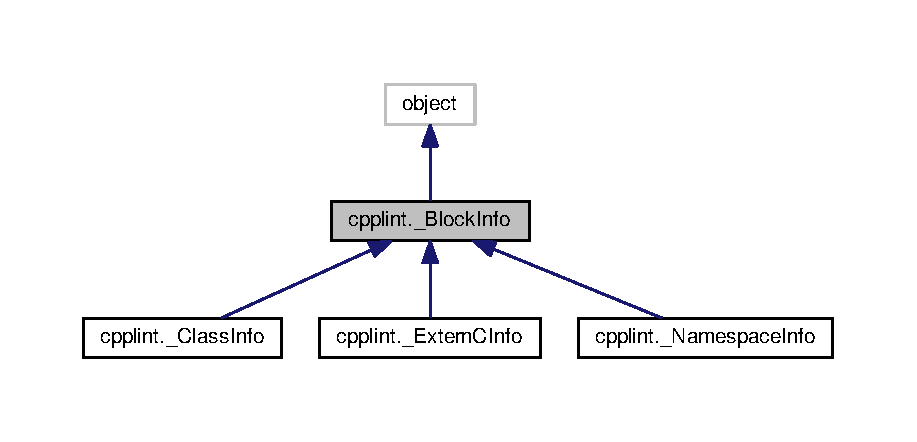
\includegraphics[width=350pt]{classcpplint_1_1__BlockInfo__inherit__graph}
\end{center}
\end{figure}


Collaboration diagram for cpplint.\+\_\+\+Block\+Info\+:\nopagebreak
\begin{figure}[H]
\begin{center}
\leavevmode
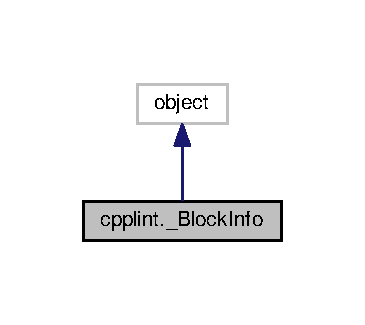
\includegraphics[width=175pt]{classcpplint_1_1__BlockInfo__coll__graph}
\end{center}
\end{figure}
\subsection*{Public Member Functions}
\begin{DoxyCompactItemize}
\item 
def \hyperlink{classcpplint_1_1__BlockInfo_ab1663260e978a348a4ff2ab9d7324587}{\+\_\+\+\_\+init\+\_\+\+\_\+} (self, linenum, \hyperlink{classcpplint_1_1__BlockInfo_aa974539217437751383ad20896c974d7}{seen\+\_\+open\+\_\+brace})
\item 
def \hyperlink{classcpplint_1_1__BlockInfo_af316a9e3623b45bd07079166be67582c}{Check\+Begin} (self, filename, clean\+\_\+lines, linenum, error)
\item 
def \hyperlink{classcpplint_1_1__BlockInfo_ae504a3429de136eebf85f32fcae6a8ca}{Check\+End} (self, filename, clean\+\_\+lines, linenum, error)
\item 
def \hyperlink{classcpplint_1_1__BlockInfo_ab3e06a94a38d7397ce6a4faa094010d4}{Is\+Block\+Info} (self)
\end{DoxyCompactItemize}
\subsection*{Public Attributes}
\begin{DoxyCompactItemize}
\item 
\hyperlink{classcpplint_1_1__BlockInfo_a81d316f03e42aebbfe0636f905c4c291}{starting\+\_\+linenum}
\item 
\hyperlink{classcpplint_1_1__BlockInfo_aa974539217437751383ad20896c974d7}{seen\+\_\+open\+\_\+brace}
\item 
\hyperlink{classcpplint_1_1__BlockInfo_a02a0b48995a599f6b2bbaa6f16cca98a}{open\+\_\+parentheses}
\item 
\hyperlink{classcpplint_1_1__BlockInfo_aad762ef7088f2f556a75c9a80006f4db}{inline\+\_\+asm}
\item 
\hyperlink{classcpplint_1_1__BlockInfo_a120822b07db37b3480a573ec29ee4457}{check\+\_\+namespace\+\_\+indentation}
\end{DoxyCompactItemize}


\subsection{Detailed Description}
\begin{DoxyVerb}Stores information about a generic block of code.\end{DoxyVerb}
 

\subsection{Constructor \& Destructor Documentation}
\index{cpplint\+::\+\_\+\+Block\+Info@{cpplint\+::\+\_\+\+Block\+Info}!\+\_\+\+\_\+init\+\_\+\+\_\+@{\+\_\+\+\_\+init\+\_\+\+\_\+}}
\index{\+\_\+\+\_\+init\+\_\+\+\_\+@{\+\_\+\+\_\+init\+\_\+\+\_\+}!cpplint\+::\+\_\+\+Block\+Info@{cpplint\+::\+\_\+\+Block\+Info}}
\subsubsection[{\texorpdfstring{\+\_\+\+\_\+init\+\_\+\+\_\+(self, linenum, seen\+\_\+open\+\_\+brace)}{__init__(self, linenum, seen_open_brace)}}]{\setlength{\rightskip}{0pt plus 5cm}def cpplint.\+\_\+\+Block\+Info.\+\_\+\+\_\+init\+\_\+\+\_\+ (
\begin{DoxyParamCaption}
\item[{}]{self, }
\item[{}]{linenum, }
\item[{}]{seen\+\_\+open\+\_\+brace}
\end{DoxyParamCaption}
)}\hypertarget{classcpplint_1_1__BlockInfo_ab1663260e978a348a4ff2ab9d7324587}{}\label{classcpplint_1_1__BlockInfo_ab1663260e978a348a4ff2ab9d7324587}


\subsection{Member Function Documentation}
\index{cpplint\+::\+\_\+\+Block\+Info@{cpplint\+::\+\_\+\+Block\+Info}!Check\+Begin@{Check\+Begin}}
\index{Check\+Begin@{Check\+Begin}!cpplint\+::\+\_\+\+Block\+Info@{cpplint\+::\+\_\+\+Block\+Info}}
\subsubsection[{\texorpdfstring{Check\+Begin(self, filename, clean\+\_\+lines, linenum, error)}{CheckBegin(self, filename, clean_lines, linenum, error)}}]{\setlength{\rightskip}{0pt plus 5cm}def cpplint.\+\_\+\+Block\+Info.\+Check\+Begin (
\begin{DoxyParamCaption}
\item[{}]{self, }
\item[{}]{filename, }
\item[{}]{clean\+\_\+lines, }
\item[{}]{linenum, }
\item[{}]{error}
\end{DoxyParamCaption}
)}\hypertarget{classcpplint_1_1__BlockInfo_af316a9e3623b45bd07079166be67582c}{}\label{classcpplint_1_1__BlockInfo_af316a9e3623b45bd07079166be67582c}
\begin{DoxyVerb}Run checks that applies to text up to the opening brace.

This is mostly for checking the text after the class identifier
and the "{", usually where the base class is specified.  For other
blocks, there isn't much to check, so we always pass.

Args:
  filename: The name of the current file.
  clean_lines: A CleansedLines instance containing the file.
  linenum: The number of the line to check.
  error: The function to call with any errors found.
\end{DoxyVerb}
 \index{cpplint\+::\+\_\+\+Block\+Info@{cpplint\+::\+\_\+\+Block\+Info}!Check\+End@{Check\+End}}
\index{Check\+End@{Check\+End}!cpplint\+::\+\_\+\+Block\+Info@{cpplint\+::\+\_\+\+Block\+Info}}
\subsubsection[{\texorpdfstring{Check\+End(self, filename, clean\+\_\+lines, linenum, error)}{CheckEnd(self, filename, clean_lines, linenum, error)}}]{\setlength{\rightskip}{0pt plus 5cm}def cpplint.\+\_\+\+Block\+Info.\+Check\+End (
\begin{DoxyParamCaption}
\item[{}]{self, }
\item[{}]{filename, }
\item[{}]{clean\+\_\+lines, }
\item[{}]{linenum, }
\item[{}]{error}
\end{DoxyParamCaption}
)}\hypertarget{classcpplint_1_1__BlockInfo_ae504a3429de136eebf85f32fcae6a8ca}{}\label{classcpplint_1_1__BlockInfo_ae504a3429de136eebf85f32fcae6a8ca}
\begin{DoxyVerb}Run checks that applies to text after the closing brace.

This is mostly used for checking end of namespace comments.

Args:
  filename: The name of the current file.
  clean_lines: A CleansedLines instance containing the file.
  linenum: The number of the line to check.
  error: The function to call with any errors found.
\end{DoxyVerb}
 \index{cpplint\+::\+\_\+\+Block\+Info@{cpplint\+::\+\_\+\+Block\+Info}!Is\+Block\+Info@{Is\+Block\+Info}}
\index{Is\+Block\+Info@{Is\+Block\+Info}!cpplint\+::\+\_\+\+Block\+Info@{cpplint\+::\+\_\+\+Block\+Info}}
\subsubsection[{\texorpdfstring{Is\+Block\+Info(self)}{IsBlockInfo(self)}}]{\setlength{\rightskip}{0pt plus 5cm}def cpplint.\+\_\+\+Block\+Info.\+Is\+Block\+Info (
\begin{DoxyParamCaption}
\item[{}]{self}
\end{DoxyParamCaption}
)}\hypertarget{classcpplint_1_1__BlockInfo_ab3e06a94a38d7397ce6a4faa094010d4}{}\label{classcpplint_1_1__BlockInfo_ab3e06a94a38d7397ce6a4faa094010d4}
\begin{DoxyVerb}Returns true if this block is a _BlockInfo.

This is convenient for verifying that an object is an instance of
a _BlockInfo, but not an instance of any of the derived classes.

Returns:
  True for this class, False for derived classes.
\end{DoxyVerb}
 

\subsection{Member Data Documentation}
\index{cpplint\+::\+\_\+\+Block\+Info@{cpplint\+::\+\_\+\+Block\+Info}!check\+\_\+namespace\+\_\+indentation@{check\+\_\+namespace\+\_\+indentation}}
\index{check\+\_\+namespace\+\_\+indentation@{check\+\_\+namespace\+\_\+indentation}!cpplint\+::\+\_\+\+Block\+Info@{cpplint\+::\+\_\+\+Block\+Info}}
\subsubsection[{\texorpdfstring{check\+\_\+namespace\+\_\+indentation}{check_namespace_indentation}}]{\setlength{\rightskip}{0pt plus 5cm}cpplint.\+\_\+\+Block\+Info.\+check\+\_\+namespace\+\_\+indentation}\hypertarget{classcpplint_1_1__BlockInfo_a120822b07db37b3480a573ec29ee4457}{}\label{classcpplint_1_1__BlockInfo_a120822b07db37b3480a573ec29ee4457}
\index{cpplint\+::\+\_\+\+Block\+Info@{cpplint\+::\+\_\+\+Block\+Info}!inline\+\_\+asm@{inline\+\_\+asm}}
\index{inline\+\_\+asm@{inline\+\_\+asm}!cpplint\+::\+\_\+\+Block\+Info@{cpplint\+::\+\_\+\+Block\+Info}}
\subsubsection[{\texorpdfstring{inline\+\_\+asm}{inline_asm}}]{\setlength{\rightskip}{0pt plus 5cm}cpplint.\+\_\+\+Block\+Info.\+inline\+\_\+asm}\hypertarget{classcpplint_1_1__BlockInfo_aad762ef7088f2f556a75c9a80006f4db}{}\label{classcpplint_1_1__BlockInfo_aad762ef7088f2f556a75c9a80006f4db}
\index{cpplint\+::\+\_\+\+Block\+Info@{cpplint\+::\+\_\+\+Block\+Info}!open\+\_\+parentheses@{open\+\_\+parentheses}}
\index{open\+\_\+parentheses@{open\+\_\+parentheses}!cpplint\+::\+\_\+\+Block\+Info@{cpplint\+::\+\_\+\+Block\+Info}}
\subsubsection[{\texorpdfstring{open\+\_\+parentheses}{open_parentheses}}]{\setlength{\rightskip}{0pt plus 5cm}cpplint.\+\_\+\+Block\+Info.\+open\+\_\+parentheses}\hypertarget{classcpplint_1_1__BlockInfo_a02a0b48995a599f6b2bbaa6f16cca98a}{}\label{classcpplint_1_1__BlockInfo_a02a0b48995a599f6b2bbaa6f16cca98a}
\index{cpplint\+::\+\_\+\+Block\+Info@{cpplint\+::\+\_\+\+Block\+Info}!seen\+\_\+open\+\_\+brace@{seen\+\_\+open\+\_\+brace}}
\index{seen\+\_\+open\+\_\+brace@{seen\+\_\+open\+\_\+brace}!cpplint\+::\+\_\+\+Block\+Info@{cpplint\+::\+\_\+\+Block\+Info}}
\subsubsection[{\texorpdfstring{seen\+\_\+open\+\_\+brace}{seen_open_brace}}]{\setlength{\rightskip}{0pt plus 5cm}cpplint.\+\_\+\+Block\+Info.\+seen\+\_\+open\+\_\+brace}\hypertarget{classcpplint_1_1__BlockInfo_aa974539217437751383ad20896c974d7}{}\label{classcpplint_1_1__BlockInfo_aa974539217437751383ad20896c974d7}
\index{cpplint\+::\+\_\+\+Block\+Info@{cpplint\+::\+\_\+\+Block\+Info}!starting\+\_\+linenum@{starting\+\_\+linenum}}
\index{starting\+\_\+linenum@{starting\+\_\+linenum}!cpplint\+::\+\_\+\+Block\+Info@{cpplint\+::\+\_\+\+Block\+Info}}
\subsubsection[{\texorpdfstring{starting\+\_\+linenum}{starting_linenum}}]{\setlength{\rightskip}{0pt plus 5cm}cpplint.\+\_\+\+Block\+Info.\+starting\+\_\+linenum}\hypertarget{classcpplint_1_1__BlockInfo_a81d316f03e42aebbfe0636f905c4c291}{}\label{classcpplint_1_1__BlockInfo_a81d316f03e42aebbfe0636f905c4c291}


The documentation for this class was generated from the following file\+:\begin{DoxyCompactItemize}
\item 
\hyperlink{cpplint_8py}{cpplint.\+py}\end{DoxyCompactItemize}

\hypertarget{classcpplint_1_1__ClassInfo}{}\section{cpplint.\+\_\+\+Class\+Info Class Reference}
\label{classcpplint_1_1__ClassInfo}\index{cpplint.\+\_\+\+Class\+Info@{cpplint.\+\_\+\+Class\+Info}}


Inheritance diagram for cpplint.\+\_\+\+Class\+Info\+:\nopagebreak
\begin{figure}[H]
\begin{center}
\leavevmode
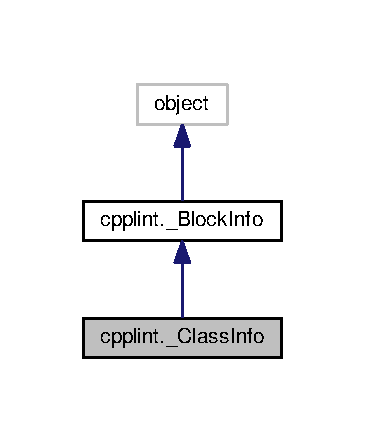
\includegraphics[width=175pt]{classcpplint_1_1__ClassInfo__inherit__graph}
\end{center}
\end{figure}


Collaboration diagram for cpplint.\+\_\+\+Class\+Info\+:\nopagebreak
\begin{figure}[H]
\begin{center}
\leavevmode
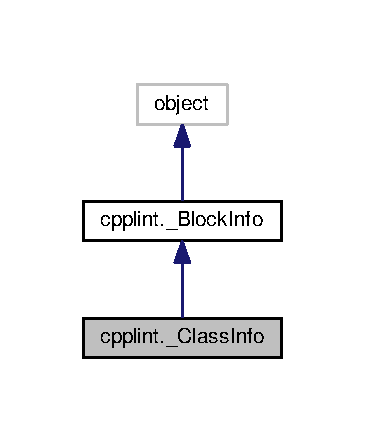
\includegraphics[width=175pt]{classcpplint_1_1__ClassInfo__coll__graph}
\end{center}
\end{figure}
\subsection*{Public Member Functions}
\begin{DoxyCompactItemize}
\item 
def \hyperlink{classcpplint_1_1__ClassInfo_a549b13e77acbe712f79a2d2b2c98ff7d}{\+\_\+\+\_\+init\+\_\+\+\_\+} (self, \hyperlink{classcpplint_1_1__ClassInfo_a3de5f207d3449d735d15ebca779fe336}{name}, class\+\_\+or\+\_\+struct, clean\+\_\+lines, linenum)
\item 
def \hyperlink{classcpplint_1_1__ClassInfo_abed47237f2e7416ca51cb220cfad6c1b}{Check\+Begin} (self, filename, clean\+\_\+lines, linenum, error)
\item 
def \hyperlink{classcpplint_1_1__ClassInfo_a8a61461a72928bc6ce62a9b75b770fec}{Check\+End} (self, filename, clean\+\_\+lines, linenum, error)
\end{DoxyCompactItemize}
\subsection*{Public Attributes}
\begin{DoxyCompactItemize}
\item 
\hyperlink{classcpplint_1_1__ClassInfo_a3de5f207d3449d735d15ebca779fe336}{name}
\item 
\hyperlink{classcpplint_1_1__ClassInfo_a8cace481686fbbb35a1da552646aa9f4}{is\+\_\+derived}
\item 
\hyperlink{classcpplint_1_1__ClassInfo_a0ead95c17ac0b293d0d371eb7b414bd9}{check\+\_\+namespace\+\_\+indentation}
\item 
\hyperlink{classcpplint_1_1__ClassInfo_aef1251c699b50c6603ce38ca8cce414c}{access}
\item 
\hyperlink{classcpplint_1_1__ClassInfo_a57b443f42838d73183921d661b6fe4ef}{is\+\_\+struct}
\item 
\hyperlink{classcpplint_1_1__ClassInfo_adc7d328734cc58fe46a3a3f323a09f4a}{class\+\_\+indent}
\item 
\hyperlink{classcpplint_1_1__ClassInfo_a72e0f4576cdcb6f3886ed52e2affbc75}{last\+\_\+line}
\end{DoxyCompactItemize}


\subsection{Detailed Description}
\begin{DoxyVerb}Stores information about a class.\end{DoxyVerb}
 

\subsection{Constructor \& Destructor Documentation}
\index{cpplint\+::\+\_\+\+Class\+Info@{cpplint\+::\+\_\+\+Class\+Info}!\+\_\+\+\_\+init\+\_\+\+\_\+@{\+\_\+\+\_\+init\+\_\+\+\_\+}}
\index{\+\_\+\+\_\+init\+\_\+\+\_\+@{\+\_\+\+\_\+init\+\_\+\+\_\+}!cpplint\+::\+\_\+\+Class\+Info@{cpplint\+::\+\_\+\+Class\+Info}}
\subsubsection[{\texorpdfstring{\+\_\+\+\_\+init\+\_\+\+\_\+(self, name, class\+\_\+or\+\_\+struct, clean\+\_\+lines, linenum)}{__init__(self, name, class_or_struct, clean_lines, linenum)}}]{\setlength{\rightskip}{0pt plus 5cm}def cpplint.\+\_\+\+Class\+Info.\+\_\+\+\_\+init\+\_\+\+\_\+ (
\begin{DoxyParamCaption}
\item[{}]{self, }
\item[{}]{name, }
\item[{}]{class\+\_\+or\+\_\+struct, }
\item[{}]{clean\+\_\+lines, }
\item[{}]{linenum}
\end{DoxyParamCaption}
)}\hypertarget{classcpplint_1_1__ClassInfo_a549b13e77acbe712f79a2d2b2c98ff7d}{}\label{classcpplint_1_1__ClassInfo_a549b13e77acbe712f79a2d2b2c98ff7d}


\subsection{Member Function Documentation}
\index{cpplint\+::\+\_\+\+Class\+Info@{cpplint\+::\+\_\+\+Class\+Info}!Check\+Begin@{Check\+Begin}}
\index{Check\+Begin@{Check\+Begin}!cpplint\+::\+\_\+\+Class\+Info@{cpplint\+::\+\_\+\+Class\+Info}}
\subsubsection[{\texorpdfstring{Check\+Begin(self, filename, clean\+\_\+lines, linenum, error)}{CheckBegin(self, filename, clean_lines, linenum, error)}}]{\setlength{\rightskip}{0pt plus 5cm}def cpplint.\+\_\+\+Class\+Info.\+Check\+Begin (
\begin{DoxyParamCaption}
\item[{}]{self, }
\item[{}]{filename, }
\item[{}]{clean\+\_\+lines, }
\item[{}]{linenum, }
\item[{}]{error}
\end{DoxyParamCaption}
)}\hypertarget{classcpplint_1_1__ClassInfo_abed47237f2e7416ca51cb220cfad6c1b}{}\label{classcpplint_1_1__ClassInfo_abed47237f2e7416ca51cb220cfad6c1b}
\index{cpplint\+::\+\_\+\+Class\+Info@{cpplint\+::\+\_\+\+Class\+Info}!Check\+End@{Check\+End}}
\index{Check\+End@{Check\+End}!cpplint\+::\+\_\+\+Class\+Info@{cpplint\+::\+\_\+\+Class\+Info}}
\subsubsection[{\texorpdfstring{Check\+End(self, filename, clean\+\_\+lines, linenum, error)}{CheckEnd(self, filename, clean_lines, linenum, error)}}]{\setlength{\rightskip}{0pt plus 5cm}def cpplint.\+\_\+\+Class\+Info.\+Check\+End (
\begin{DoxyParamCaption}
\item[{}]{self, }
\item[{}]{filename, }
\item[{}]{clean\+\_\+lines, }
\item[{}]{linenum, }
\item[{}]{error}
\end{DoxyParamCaption}
)}\hypertarget{classcpplint_1_1__ClassInfo_a8a61461a72928bc6ce62a9b75b770fec}{}\label{classcpplint_1_1__ClassInfo_a8a61461a72928bc6ce62a9b75b770fec}


\subsection{Member Data Documentation}
\index{cpplint\+::\+\_\+\+Class\+Info@{cpplint\+::\+\_\+\+Class\+Info}!access@{access}}
\index{access@{access}!cpplint\+::\+\_\+\+Class\+Info@{cpplint\+::\+\_\+\+Class\+Info}}
\subsubsection[{\texorpdfstring{access}{access}}]{\setlength{\rightskip}{0pt plus 5cm}cpplint.\+\_\+\+Class\+Info.\+access}\hypertarget{classcpplint_1_1__ClassInfo_aef1251c699b50c6603ce38ca8cce414c}{}\label{classcpplint_1_1__ClassInfo_aef1251c699b50c6603ce38ca8cce414c}
\index{cpplint\+::\+\_\+\+Class\+Info@{cpplint\+::\+\_\+\+Class\+Info}!check\+\_\+namespace\+\_\+indentation@{check\+\_\+namespace\+\_\+indentation}}
\index{check\+\_\+namespace\+\_\+indentation@{check\+\_\+namespace\+\_\+indentation}!cpplint\+::\+\_\+\+Class\+Info@{cpplint\+::\+\_\+\+Class\+Info}}
\subsubsection[{\texorpdfstring{check\+\_\+namespace\+\_\+indentation}{check_namespace_indentation}}]{\setlength{\rightskip}{0pt plus 5cm}cpplint.\+\_\+\+Class\+Info.\+check\+\_\+namespace\+\_\+indentation}\hypertarget{classcpplint_1_1__ClassInfo_a0ead95c17ac0b293d0d371eb7b414bd9}{}\label{classcpplint_1_1__ClassInfo_a0ead95c17ac0b293d0d371eb7b414bd9}
\index{cpplint\+::\+\_\+\+Class\+Info@{cpplint\+::\+\_\+\+Class\+Info}!class\+\_\+indent@{class\+\_\+indent}}
\index{class\+\_\+indent@{class\+\_\+indent}!cpplint\+::\+\_\+\+Class\+Info@{cpplint\+::\+\_\+\+Class\+Info}}
\subsubsection[{\texorpdfstring{class\+\_\+indent}{class_indent}}]{\setlength{\rightskip}{0pt plus 5cm}cpplint.\+\_\+\+Class\+Info.\+class\+\_\+indent}\hypertarget{classcpplint_1_1__ClassInfo_adc7d328734cc58fe46a3a3f323a09f4a}{}\label{classcpplint_1_1__ClassInfo_adc7d328734cc58fe46a3a3f323a09f4a}
\index{cpplint\+::\+\_\+\+Class\+Info@{cpplint\+::\+\_\+\+Class\+Info}!is\+\_\+derived@{is\+\_\+derived}}
\index{is\+\_\+derived@{is\+\_\+derived}!cpplint\+::\+\_\+\+Class\+Info@{cpplint\+::\+\_\+\+Class\+Info}}
\subsubsection[{\texorpdfstring{is\+\_\+derived}{is_derived}}]{\setlength{\rightskip}{0pt plus 5cm}cpplint.\+\_\+\+Class\+Info.\+is\+\_\+derived}\hypertarget{classcpplint_1_1__ClassInfo_a8cace481686fbbb35a1da552646aa9f4}{}\label{classcpplint_1_1__ClassInfo_a8cace481686fbbb35a1da552646aa9f4}
\index{cpplint\+::\+\_\+\+Class\+Info@{cpplint\+::\+\_\+\+Class\+Info}!is\+\_\+struct@{is\+\_\+struct}}
\index{is\+\_\+struct@{is\+\_\+struct}!cpplint\+::\+\_\+\+Class\+Info@{cpplint\+::\+\_\+\+Class\+Info}}
\subsubsection[{\texorpdfstring{is\+\_\+struct}{is_struct}}]{\setlength{\rightskip}{0pt plus 5cm}cpplint.\+\_\+\+Class\+Info.\+is\+\_\+struct}\hypertarget{classcpplint_1_1__ClassInfo_a57b443f42838d73183921d661b6fe4ef}{}\label{classcpplint_1_1__ClassInfo_a57b443f42838d73183921d661b6fe4ef}
\index{cpplint\+::\+\_\+\+Class\+Info@{cpplint\+::\+\_\+\+Class\+Info}!last\+\_\+line@{last\+\_\+line}}
\index{last\+\_\+line@{last\+\_\+line}!cpplint\+::\+\_\+\+Class\+Info@{cpplint\+::\+\_\+\+Class\+Info}}
\subsubsection[{\texorpdfstring{last\+\_\+line}{last_line}}]{\setlength{\rightskip}{0pt plus 5cm}cpplint.\+\_\+\+Class\+Info.\+last\+\_\+line}\hypertarget{classcpplint_1_1__ClassInfo_a72e0f4576cdcb6f3886ed52e2affbc75}{}\label{classcpplint_1_1__ClassInfo_a72e0f4576cdcb6f3886ed52e2affbc75}
\index{cpplint\+::\+\_\+\+Class\+Info@{cpplint\+::\+\_\+\+Class\+Info}!name@{name}}
\index{name@{name}!cpplint\+::\+\_\+\+Class\+Info@{cpplint\+::\+\_\+\+Class\+Info}}
\subsubsection[{\texorpdfstring{name}{name}}]{\setlength{\rightskip}{0pt plus 5cm}cpplint.\+\_\+\+Class\+Info.\+name}\hypertarget{classcpplint_1_1__ClassInfo_a3de5f207d3449d735d15ebca779fe336}{}\label{classcpplint_1_1__ClassInfo_a3de5f207d3449d735d15ebca779fe336}


The documentation for this class was generated from the following file\+:\begin{DoxyCompactItemize}
\item 
\hyperlink{cpplint_8py}{cpplint.\+py}\end{DoxyCompactItemize}

\hypertarget{classcpplint_1_1__CppLintState}{}\section{cpplint.\+\_\+\+Cpp\+Lint\+State Class Reference}
\label{classcpplint_1_1__CppLintState}\index{cpplint.\+\_\+\+Cpp\+Lint\+State@{cpplint.\+\_\+\+Cpp\+Lint\+State}}


Inheritance diagram for cpplint.\+\_\+\+Cpp\+Lint\+State\+:\nopagebreak
\begin{figure}[H]
\begin{center}
\leavevmode
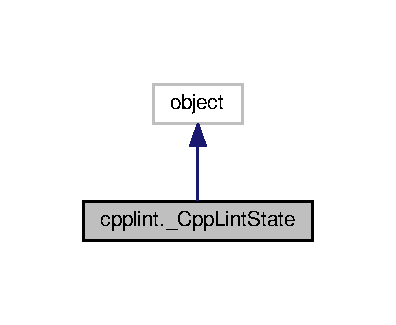
\includegraphics[width=190pt]{classcpplint_1_1__CppLintState__inherit__graph}
\end{center}
\end{figure}


Collaboration diagram for cpplint.\+\_\+\+Cpp\+Lint\+State\+:\nopagebreak
\begin{figure}[H]
\begin{center}
\leavevmode
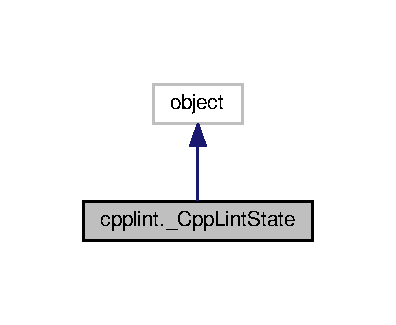
\includegraphics[width=190pt]{classcpplint_1_1__CppLintState__coll__graph}
\end{center}
\end{figure}
\subsection*{Public Member Functions}
\begin{DoxyCompactItemize}
\item 
def \hyperlink{classcpplint_1_1__CppLintState_a9cc2db6b8d2e3b757fc48fb3c2fd4d8b}{\+\_\+\+\_\+init\+\_\+\+\_\+} (self)
\item 
def \hyperlink{classcpplint_1_1__CppLintState_ab43553d2e2027b58d08a7001c71c0902}{Set\+Output\+Format} (self, \hyperlink{classcpplint_1_1__CppLintState_a5c68ca79b0ff9b2fba1c488a7b2bd3f0}{output\+\_\+format})
\item 
def \hyperlink{classcpplint_1_1__CppLintState_ad4f97c907cc79e8d60237d0327830588}{Set\+Verbose\+Level} (self, level)
\item 
def \hyperlink{classcpplint_1_1__CppLintState_ac2503f2d8a357edd3ca648d219c7317e}{Set\+Counting\+Style} (self, counting\+\_\+style)
\item 
def \hyperlink{classcpplint_1_1__CppLintState_a359d4516eac0c1dce6223cf18181ac80}{Set\+Filters} (self, \hyperlink{classcpplint_1_1__CppLintState_a8443105b9623383ab75fa242009c006e}{filters})
\item 
def \hyperlink{classcpplint_1_1__CppLintState_a248c70895572f2468d3c842faff2f285}{Add\+Filters} (self, \hyperlink{classcpplint_1_1__CppLintState_a8443105b9623383ab75fa242009c006e}{filters})
\item 
def \hyperlink{classcpplint_1_1__CppLintState_a2444e784910e03681de22f43d4077dd1}{Backup\+Filters} (self)
\item 
def \hyperlink{classcpplint_1_1__CppLintState_a7a9c9fdfe033ebe1933450b4ae524598}{Restore\+Filters} (self)
\item 
def \hyperlink{classcpplint_1_1__CppLintState_ab802596abd5fba5e290e090388b6842a}{Reset\+Error\+Counts} (self)
\item 
def \hyperlink{classcpplint_1_1__CppLintState_a27a33a5049850d52cc8aef3478ca445a}{Increment\+Error\+Count} (self, category)
\item 
def \hyperlink{classcpplint_1_1__CppLintState_a3149156b00f8d53e5625256e3df2b4f0}{Print\+Error\+Counts} (self)
\end{DoxyCompactItemize}
\subsection*{Public Attributes}
\begin{DoxyCompactItemize}
\item 
\hyperlink{classcpplint_1_1__CppLintState_a94328754c2f7481f4da9757a9dede308}{verbose\+\_\+level}
\item 
\hyperlink{classcpplint_1_1__CppLintState_a4039ff9668057eff4549b99905ce753b}{error\+\_\+count}
\item 
\hyperlink{classcpplint_1_1__CppLintState_a8443105b9623383ab75fa242009c006e}{filters}
\item 
\hyperlink{classcpplint_1_1__CppLintState_acd4f4157637d141a4de63bf10d2ca755}{counting}
\item 
\hyperlink{classcpplint_1_1__CppLintState_afb33527113706b5fcae07d680d8cec99}{errors\+\_\+by\+\_\+category}
\item 
\hyperlink{classcpplint_1_1__CppLintState_a5c68ca79b0ff9b2fba1c488a7b2bd3f0}{output\+\_\+format}
\end{DoxyCompactItemize}


\subsection{Detailed Description}
\begin{DoxyVerb}Maintains module-wide state..\end{DoxyVerb}
 

\subsection{Constructor \& Destructor Documentation}
\index{cpplint\+::\+\_\+\+Cpp\+Lint\+State@{cpplint\+::\+\_\+\+Cpp\+Lint\+State}!\+\_\+\+\_\+init\+\_\+\+\_\+@{\+\_\+\+\_\+init\+\_\+\+\_\+}}
\index{\+\_\+\+\_\+init\+\_\+\+\_\+@{\+\_\+\+\_\+init\+\_\+\+\_\+}!cpplint\+::\+\_\+\+Cpp\+Lint\+State@{cpplint\+::\+\_\+\+Cpp\+Lint\+State}}
\subsubsection[{\texorpdfstring{\+\_\+\+\_\+init\+\_\+\+\_\+(self)}{__init__(self)}}]{\setlength{\rightskip}{0pt plus 5cm}def cpplint.\+\_\+\+Cpp\+Lint\+State.\+\_\+\+\_\+init\+\_\+\+\_\+ (
\begin{DoxyParamCaption}
\item[{}]{self}
\end{DoxyParamCaption}
)}\hypertarget{classcpplint_1_1__CppLintState_a9cc2db6b8d2e3b757fc48fb3c2fd4d8b}{}\label{classcpplint_1_1__CppLintState_a9cc2db6b8d2e3b757fc48fb3c2fd4d8b}


\subsection{Member Function Documentation}
\index{cpplint\+::\+\_\+\+Cpp\+Lint\+State@{cpplint\+::\+\_\+\+Cpp\+Lint\+State}!Add\+Filters@{Add\+Filters}}
\index{Add\+Filters@{Add\+Filters}!cpplint\+::\+\_\+\+Cpp\+Lint\+State@{cpplint\+::\+\_\+\+Cpp\+Lint\+State}}
\subsubsection[{\texorpdfstring{Add\+Filters(self, filters)}{AddFilters(self, filters)}}]{\setlength{\rightskip}{0pt plus 5cm}def cpplint.\+\_\+\+Cpp\+Lint\+State.\+Add\+Filters (
\begin{DoxyParamCaption}
\item[{}]{self, }
\item[{}]{filters}
\end{DoxyParamCaption}
)}\hypertarget{classcpplint_1_1__CppLintState_a248c70895572f2468d3c842faff2f285}{}\label{classcpplint_1_1__CppLintState_a248c70895572f2468d3c842faff2f285}
\begin{DoxyVerb}Adds more filters to the existing list of error-message filters. \end{DoxyVerb}
 \index{cpplint\+::\+\_\+\+Cpp\+Lint\+State@{cpplint\+::\+\_\+\+Cpp\+Lint\+State}!Backup\+Filters@{Backup\+Filters}}
\index{Backup\+Filters@{Backup\+Filters}!cpplint\+::\+\_\+\+Cpp\+Lint\+State@{cpplint\+::\+\_\+\+Cpp\+Lint\+State}}
\subsubsection[{\texorpdfstring{Backup\+Filters(self)}{BackupFilters(self)}}]{\setlength{\rightskip}{0pt plus 5cm}def cpplint.\+\_\+\+Cpp\+Lint\+State.\+Backup\+Filters (
\begin{DoxyParamCaption}
\item[{}]{self}
\end{DoxyParamCaption}
)}\hypertarget{classcpplint_1_1__CppLintState_a2444e784910e03681de22f43d4077dd1}{}\label{classcpplint_1_1__CppLintState_a2444e784910e03681de22f43d4077dd1}
\begin{DoxyVerb}Saves the current filter list to backup storage.\end{DoxyVerb}
 \index{cpplint\+::\+\_\+\+Cpp\+Lint\+State@{cpplint\+::\+\_\+\+Cpp\+Lint\+State}!Increment\+Error\+Count@{Increment\+Error\+Count}}
\index{Increment\+Error\+Count@{Increment\+Error\+Count}!cpplint\+::\+\_\+\+Cpp\+Lint\+State@{cpplint\+::\+\_\+\+Cpp\+Lint\+State}}
\subsubsection[{\texorpdfstring{Increment\+Error\+Count(self, category)}{IncrementErrorCount(self, category)}}]{\setlength{\rightskip}{0pt plus 5cm}def cpplint.\+\_\+\+Cpp\+Lint\+State.\+Increment\+Error\+Count (
\begin{DoxyParamCaption}
\item[{}]{self, }
\item[{}]{category}
\end{DoxyParamCaption}
)}\hypertarget{classcpplint_1_1__CppLintState_a27a33a5049850d52cc8aef3478ca445a}{}\label{classcpplint_1_1__CppLintState_a27a33a5049850d52cc8aef3478ca445a}
\begin{DoxyVerb}Bumps the module's error statistic.\end{DoxyVerb}
 \index{cpplint\+::\+\_\+\+Cpp\+Lint\+State@{cpplint\+::\+\_\+\+Cpp\+Lint\+State}!Print\+Error\+Counts@{Print\+Error\+Counts}}
\index{Print\+Error\+Counts@{Print\+Error\+Counts}!cpplint\+::\+\_\+\+Cpp\+Lint\+State@{cpplint\+::\+\_\+\+Cpp\+Lint\+State}}
\subsubsection[{\texorpdfstring{Print\+Error\+Counts(self)}{PrintErrorCounts(self)}}]{\setlength{\rightskip}{0pt plus 5cm}def cpplint.\+\_\+\+Cpp\+Lint\+State.\+Print\+Error\+Counts (
\begin{DoxyParamCaption}
\item[{}]{self}
\end{DoxyParamCaption}
)}\hypertarget{classcpplint_1_1__CppLintState_a3149156b00f8d53e5625256e3df2b4f0}{}\label{classcpplint_1_1__CppLintState_a3149156b00f8d53e5625256e3df2b4f0}
\begin{DoxyVerb}Print a summary of errors by category, and the total.\end{DoxyVerb}
 \index{cpplint\+::\+\_\+\+Cpp\+Lint\+State@{cpplint\+::\+\_\+\+Cpp\+Lint\+State}!Reset\+Error\+Counts@{Reset\+Error\+Counts}}
\index{Reset\+Error\+Counts@{Reset\+Error\+Counts}!cpplint\+::\+\_\+\+Cpp\+Lint\+State@{cpplint\+::\+\_\+\+Cpp\+Lint\+State}}
\subsubsection[{\texorpdfstring{Reset\+Error\+Counts(self)}{ResetErrorCounts(self)}}]{\setlength{\rightskip}{0pt plus 5cm}def cpplint.\+\_\+\+Cpp\+Lint\+State.\+Reset\+Error\+Counts (
\begin{DoxyParamCaption}
\item[{}]{self}
\end{DoxyParamCaption}
)}\hypertarget{classcpplint_1_1__CppLintState_ab802596abd5fba5e290e090388b6842a}{}\label{classcpplint_1_1__CppLintState_ab802596abd5fba5e290e090388b6842a}
\begin{DoxyVerb}Sets the module's error statistic back to zero.\end{DoxyVerb}
 \index{cpplint\+::\+\_\+\+Cpp\+Lint\+State@{cpplint\+::\+\_\+\+Cpp\+Lint\+State}!Restore\+Filters@{Restore\+Filters}}
\index{Restore\+Filters@{Restore\+Filters}!cpplint\+::\+\_\+\+Cpp\+Lint\+State@{cpplint\+::\+\_\+\+Cpp\+Lint\+State}}
\subsubsection[{\texorpdfstring{Restore\+Filters(self)}{RestoreFilters(self)}}]{\setlength{\rightskip}{0pt plus 5cm}def cpplint.\+\_\+\+Cpp\+Lint\+State.\+Restore\+Filters (
\begin{DoxyParamCaption}
\item[{}]{self}
\end{DoxyParamCaption}
)}\hypertarget{classcpplint_1_1__CppLintState_a7a9c9fdfe033ebe1933450b4ae524598}{}\label{classcpplint_1_1__CppLintState_a7a9c9fdfe033ebe1933450b4ae524598}
\begin{DoxyVerb}Restores filters previously backed up.\end{DoxyVerb}
 \index{cpplint\+::\+\_\+\+Cpp\+Lint\+State@{cpplint\+::\+\_\+\+Cpp\+Lint\+State}!Set\+Counting\+Style@{Set\+Counting\+Style}}
\index{Set\+Counting\+Style@{Set\+Counting\+Style}!cpplint\+::\+\_\+\+Cpp\+Lint\+State@{cpplint\+::\+\_\+\+Cpp\+Lint\+State}}
\subsubsection[{\texorpdfstring{Set\+Counting\+Style(self, counting\+\_\+style)}{SetCountingStyle(self, counting_style)}}]{\setlength{\rightskip}{0pt plus 5cm}def cpplint.\+\_\+\+Cpp\+Lint\+State.\+Set\+Counting\+Style (
\begin{DoxyParamCaption}
\item[{}]{self, }
\item[{}]{counting\+\_\+style}
\end{DoxyParamCaption}
)}\hypertarget{classcpplint_1_1__CppLintState_ac2503f2d8a357edd3ca648d219c7317e}{}\label{classcpplint_1_1__CppLintState_ac2503f2d8a357edd3ca648d219c7317e}
\begin{DoxyVerb}Sets the module's counting options.\end{DoxyVerb}
 \index{cpplint\+::\+\_\+\+Cpp\+Lint\+State@{cpplint\+::\+\_\+\+Cpp\+Lint\+State}!Set\+Filters@{Set\+Filters}}
\index{Set\+Filters@{Set\+Filters}!cpplint\+::\+\_\+\+Cpp\+Lint\+State@{cpplint\+::\+\_\+\+Cpp\+Lint\+State}}
\subsubsection[{\texorpdfstring{Set\+Filters(self, filters)}{SetFilters(self, filters)}}]{\setlength{\rightskip}{0pt plus 5cm}def cpplint.\+\_\+\+Cpp\+Lint\+State.\+Set\+Filters (
\begin{DoxyParamCaption}
\item[{}]{self, }
\item[{}]{filters}
\end{DoxyParamCaption}
)}\hypertarget{classcpplint_1_1__CppLintState_a359d4516eac0c1dce6223cf18181ac80}{}\label{classcpplint_1_1__CppLintState_a359d4516eac0c1dce6223cf18181ac80}
\begin{DoxyVerb}Sets the error-message filters.

These filters are applied when deciding whether to emit a given
error message.

Args:
  filters: A string of comma-separated filters (eg "+whitespace/indent").
       Each filter should start with + or -; else we die.

Raises:
  ValueError: The comma-separated filters did not all start with '+' or '-'.
          E.g. "-,+whitespace,-whitespace/indent,whitespace/badfilter"
\end{DoxyVerb}
 \index{cpplint\+::\+\_\+\+Cpp\+Lint\+State@{cpplint\+::\+\_\+\+Cpp\+Lint\+State}!Set\+Output\+Format@{Set\+Output\+Format}}
\index{Set\+Output\+Format@{Set\+Output\+Format}!cpplint\+::\+\_\+\+Cpp\+Lint\+State@{cpplint\+::\+\_\+\+Cpp\+Lint\+State}}
\subsubsection[{\texorpdfstring{Set\+Output\+Format(self, output\+\_\+format)}{SetOutputFormat(self, output_format)}}]{\setlength{\rightskip}{0pt plus 5cm}def cpplint.\+\_\+\+Cpp\+Lint\+State.\+Set\+Output\+Format (
\begin{DoxyParamCaption}
\item[{}]{self, }
\item[{}]{output\+\_\+format}
\end{DoxyParamCaption}
)}\hypertarget{classcpplint_1_1__CppLintState_ab43553d2e2027b58d08a7001c71c0902}{}\label{classcpplint_1_1__CppLintState_ab43553d2e2027b58d08a7001c71c0902}
\begin{DoxyVerb}Sets the output format for errors.\end{DoxyVerb}
 \index{cpplint\+::\+\_\+\+Cpp\+Lint\+State@{cpplint\+::\+\_\+\+Cpp\+Lint\+State}!Set\+Verbose\+Level@{Set\+Verbose\+Level}}
\index{Set\+Verbose\+Level@{Set\+Verbose\+Level}!cpplint\+::\+\_\+\+Cpp\+Lint\+State@{cpplint\+::\+\_\+\+Cpp\+Lint\+State}}
\subsubsection[{\texorpdfstring{Set\+Verbose\+Level(self, level)}{SetVerboseLevel(self, level)}}]{\setlength{\rightskip}{0pt plus 5cm}def cpplint.\+\_\+\+Cpp\+Lint\+State.\+Set\+Verbose\+Level (
\begin{DoxyParamCaption}
\item[{}]{self, }
\item[{}]{level}
\end{DoxyParamCaption}
)}\hypertarget{classcpplint_1_1__CppLintState_ad4f97c907cc79e8d60237d0327830588}{}\label{classcpplint_1_1__CppLintState_ad4f97c907cc79e8d60237d0327830588}
\begin{DoxyVerb}Sets the module's verbosity, and returns the previous setting.\end{DoxyVerb}
 

\subsection{Member Data Documentation}
\index{cpplint\+::\+\_\+\+Cpp\+Lint\+State@{cpplint\+::\+\_\+\+Cpp\+Lint\+State}!counting@{counting}}
\index{counting@{counting}!cpplint\+::\+\_\+\+Cpp\+Lint\+State@{cpplint\+::\+\_\+\+Cpp\+Lint\+State}}
\subsubsection[{\texorpdfstring{counting}{counting}}]{\setlength{\rightskip}{0pt plus 5cm}cpplint.\+\_\+\+Cpp\+Lint\+State.\+counting}\hypertarget{classcpplint_1_1__CppLintState_acd4f4157637d141a4de63bf10d2ca755}{}\label{classcpplint_1_1__CppLintState_acd4f4157637d141a4de63bf10d2ca755}
\index{cpplint\+::\+\_\+\+Cpp\+Lint\+State@{cpplint\+::\+\_\+\+Cpp\+Lint\+State}!error\+\_\+count@{error\+\_\+count}}
\index{error\+\_\+count@{error\+\_\+count}!cpplint\+::\+\_\+\+Cpp\+Lint\+State@{cpplint\+::\+\_\+\+Cpp\+Lint\+State}}
\subsubsection[{\texorpdfstring{error\+\_\+count}{error_count}}]{\setlength{\rightskip}{0pt plus 5cm}cpplint.\+\_\+\+Cpp\+Lint\+State.\+error\+\_\+count}\hypertarget{classcpplint_1_1__CppLintState_a4039ff9668057eff4549b99905ce753b}{}\label{classcpplint_1_1__CppLintState_a4039ff9668057eff4549b99905ce753b}
\index{cpplint\+::\+\_\+\+Cpp\+Lint\+State@{cpplint\+::\+\_\+\+Cpp\+Lint\+State}!errors\+\_\+by\+\_\+category@{errors\+\_\+by\+\_\+category}}
\index{errors\+\_\+by\+\_\+category@{errors\+\_\+by\+\_\+category}!cpplint\+::\+\_\+\+Cpp\+Lint\+State@{cpplint\+::\+\_\+\+Cpp\+Lint\+State}}
\subsubsection[{\texorpdfstring{errors\+\_\+by\+\_\+category}{errors_by_category}}]{\setlength{\rightskip}{0pt plus 5cm}cpplint.\+\_\+\+Cpp\+Lint\+State.\+errors\+\_\+by\+\_\+category}\hypertarget{classcpplint_1_1__CppLintState_afb33527113706b5fcae07d680d8cec99}{}\label{classcpplint_1_1__CppLintState_afb33527113706b5fcae07d680d8cec99}
\index{cpplint\+::\+\_\+\+Cpp\+Lint\+State@{cpplint\+::\+\_\+\+Cpp\+Lint\+State}!filters@{filters}}
\index{filters@{filters}!cpplint\+::\+\_\+\+Cpp\+Lint\+State@{cpplint\+::\+\_\+\+Cpp\+Lint\+State}}
\subsubsection[{\texorpdfstring{filters}{filters}}]{\setlength{\rightskip}{0pt plus 5cm}cpplint.\+\_\+\+Cpp\+Lint\+State.\+filters}\hypertarget{classcpplint_1_1__CppLintState_a8443105b9623383ab75fa242009c006e}{}\label{classcpplint_1_1__CppLintState_a8443105b9623383ab75fa242009c006e}
\index{cpplint\+::\+\_\+\+Cpp\+Lint\+State@{cpplint\+::\+\_\+\+Cpp\+Lint\+State}!output\+\_\+format@{output\+\_\+format}}
\index{output\+\_\+format@{output\+\_\+format}!cpplint\+::\+\_\+\+Cpp\+Lint\+State@{cpplint\+::\+\_\+\+Cpp\+Lint\+State}}
\subsubsection[{\texorpdfstring{output\+\_\+format}{output_format}}]{\setlength{\rightskip}{0pt plus 5cm}cpplint.\+\_\+\+Cpp\+Lint\+State.\+output\+\_\+format}\hypertarget{classcpplint_1_1__CppLintState_a5c68ca79b0ff9b2fba1c488a7b2bd3f0}{}\label{classcpplint_1_1__CppLintState_a5c68ca79b0ff9b2fba1c488a7b2bd3f0}
\index{cpplint\+::\+\_\+\+Cpp\+Lint\+State@{cpplint\+::\+\_\+\+Cpp\+Lint\+State}!verbose\+\_\+level@{verbose\+\_\+level}}
\index{verbose\+\_\+level@{verbose\+\_\+level}!cpplint\+::\+\_\+\+Cpp\+Lint\+State@{cpplint\+::\+\_\+\+Cpp\+Lint\+State}}
\subsubsection[{\texorpdfstring{verbose\+\_\+level}{verbose_level}}]{\setlength{\rightskip}{0pt plus 5cm}cpplint.\+\_\+\+Cpp\+Lint\+State.\+verbose\+\_\+level}\hypertarget{classcpplint_1_1__CppLintState_a94328754c2f7481f4da9757a9dede308}{}\label{classcpplint_1_1__CppLintState_a94328754c2f7481f4da9757a9dede308}


The documentation for this class was generated from the following file\+:\begin{DoxyCompactItemize}
\item 
\hyperlink{cpplint_8py}{cpplint.\+py}\end{DoxyCompactItemize}

\hypertarget{classcpplint_1_1__ExternCInfo}{}\section{cpplint.\+\_\+\+Extern\+C\+Info Class Reference}
\label{classcpplint_1_1__ExternCInfo}\index{cpplint.\+\_\+\+Extern\+C\+Info@{cpplint.\+\_\+\+Extern\+C\+Info}}


Inheritance diagram for cpplint.\+\_\+\+Extern\+C\+Info\+:\nopagebreak
\begin{figure}[H]
\begin{center}
\leavevmode
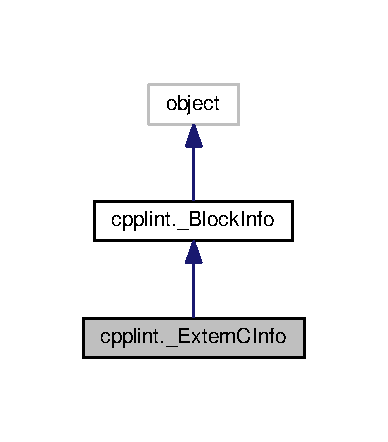
\includegraphics[width=186pt]{classcpplint_1_1__ExternCInfo__inherit__graph}
\end{center}
\end{figure}


Collaboration diagram for cpplint.\+\_\+\+Extern\+C\+Info\+:\nopagebreak
\begin{figure}[H]
\begin{center}
\leavevmode
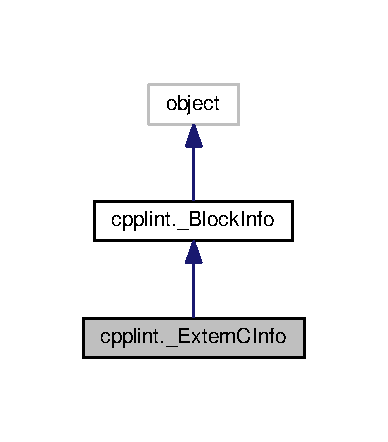
\includegraphics[width=186pt]{classcpplint_1_1__ExternCInfo__coll__graph}
\end{center}
\end{figure}
\subsection*{Public Member Functions}
\begin{DoxyCompactItemize}
\item 
def \hyperlink{classcpplint_1_1__ExternCInfo_a903a8aefdb01fd5be044f920ea110d0a}{\+\_\+\+\_\+init\+\_\+\+\_\+} (self, linenum)
\end{DoxyCompactItemize}
\subsection*{Additional Inherited Members}


\subsection{Detailed Description}
\begin{DoxyVerb}Stores information about an 'extern "C"' block.\end{DoxyVerb}
 

\subsection{Constructor \& Destructor Documentation}
\index{cpplint\+::\+\_\+\+Extern\+C\+Info@{cpplint\+::\+\_\+\+Extern\+C\+Info}!\+\_\+\+\_\+init\+\_\+\+\_\+@{\+\_\+\+\_\+init\+\_\+\+\_\+}}
\index{\+\_\+\+\_\+init\+\_\+\+\_\+@{\+\_\+\+\_\+init\+\_\+\+\_\+}!cpplint\+::\+\_\+\+Extern\+C\+Info@{cpplint\+::\+\_\+\+Extern\+C\+Info}}
\subsubsection[{\texorpdfstring{\+\_\+\+\_\+init\+\_\+\+\_\+(self, linenum)}{__init__(self, linenum)}}]{\setlength{\rightskip}{0pt plus 5cm}def cpplint.\+\_\+\+Extern\+C\+Info.\+\_\+\+\_\+init\+\_\+\+\_\+ (
\begin{DoxyParamCaption}
\item[{}]{self, }
\item[{}]{linenum}
\end{DoxyParamCaption}
)}\hypertarget{classcpplint_1_1__ExternCInfo_a903a8aefdb01fd5be044f920ea110d0a}{}\label{classcpplint_1_1__ExternCInfo_a903a8aefdb01fd5be044f920ea110d0a}


The documentation for this class was generated from the following file\+:\begin{DoxyCompactItemize}
\item 
\hyperlink{cpplint_8py}{cpplint.\+py}\end{DoxyCompactItemize}

\hypertarget{classcpplint_1_1__FunctionState}{}\section{cpplint.\+\_\+\+Function\+State Class Reference}
\label{classcpplint_1_1__FunctionState}\index{cpplint.\+\_\+\+Function\+State@{cpplint.\+\_\+\+Function\+State}}


Inheritance diagram for cpplint.\+\_\+\+Function\+State\+:\nopagebreak
\begin{figure}[H]
\begin{center}
\leavevmode
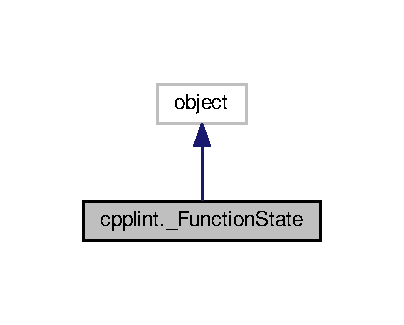
\includegraphics[width=194pt]{classcpplint_1_1__FunctionState__inherit__graph}
\end{center}
\end{figure}


Collaboration diagram for cpplint.\+\_\+\+Function\+State\+:\nopagebreak
\begin{figure}[H]
\begin{center}
\leavevmode
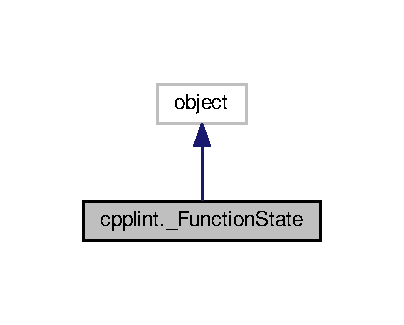
\includegraphics[width=194pt]{classcpplint_1_1__FunctionState__coll__graph}
\end{center}
\end{figure}
\subsection*{Public Member Functions}
\begin{DoxyCompactItemize}
\item 
def \hyperlink{classcpplint_1_1__FunctionState_a3f6a865710852cc74c6a7085180458ae}{\+\_\+\+\_\+init\+\_\+\+\_\+} (self)
\item 
def \hyperlink{classcpplint_1_1__FunctionState_a41215c4d73baccbb340f6d0df1c1f4b3}{Begin} (self, function\+\_\+name)
\item 
def \hyperlink{classcpplint_1_1__FunctionState_ac25c9711911ae181b091b52619cf2701}{Count} (self)
\item 
def \hyperlink{classcpplint_1_1__FunctionState_a5e4ad7d7b104038b45204ab4abf527b2}{Check} (self, error, filename, linenum)
\item 
def \hyperlink{classcpplint_1_1__FunctionState_a1ab6b0a575c25c135f9004b7fb12dc4a}{End} (self)
\end{DoxyCompactItemize}
\subsection*{Public Attributes}
\begin{DoxyCompactItemize}
\item 
\hyperlink{classcpplint_1_1__FunctionState_a8362d472591f60462184bf68b49c0efb}{in\+\_\+a\+\_\+function}
\item 
\hyperlink{classcpplint_1_1__FunctionState_a886f5d476adc81f499a711750a399aa2}{lines\+\_\+in\+\_\+function}
\item 
\hyperlink{classcpplint_1_1__FunctionState_a320674f54bd75087febc8f0d83620569}{current\+\_\+function}
\end{DoxyCompactItemize}


\subsection{Detailed Description}
\begin{DoxyVerb}Tracks current function name and the number of lines in its body.\end{DoxyVerb}
 

\subsection{Constructor \& Destructor Documentation}
\index{cpplint\+::\+\_\+\+Function\+State@{cpplint\+::\+\_\+\+Function\+State}!\+\_\+\+\_\+init\+\_\+\+\_\+@{\+\_\+\+\_\+init\+\_\+\+\_\+}}
\index{\+\_\+\+\_\+init\+\_\+\+\_\+@{\+\_\+\+\_\+init\+\_\+\+\_\+}!cpplint\+::\+\_\+\+Function\+State@{cpplint\+::\+\_\+\+Function\+State}}
\subsubsection[{\texorpdfstring{\+\_\+\+\_\+init\+\_\+\+\_\+(self)}{__init__(self)}}]{\setlength{\rightskip}{0pt plus 5cm}def cpplint.\+\_\+\+Function\+State.\+\_\+\+\_\+init\+\_\+\+\_\+ (
\begin{DoxyParamCaption}
\item[{}]{self}
\end{DoxyParamCaption}
)}\hypertarget{classcpplint_1_1__FunctionState_a3f6a865710852cc74c6a7085180458ae}{}\label{classcpplint_1_1__FunctionState_a3f6a865710852cc74c6a7085180458ae}


\subsection{Member Function Documentation}
\index{cpplint\+::\+\_\+\+Function\+State@{cpplint\+::\+\_\+\+Function\+State}!Begin@{Begin}}
\index{Begin@{Begin}!cpplint\+::\+\_\+\+Function\+State@{cpplint\+::\+\_\+\+Function\+State}}
\subsubsection[{\texorpdfstring{Begin(self, function\+\_\+name)}{Begin(self, function_name)}}]{\setlength{\rightskip}{0pt plus 5cm}def cpplint.\+\_\+\+Function\+State.\+Begin (
\begin{DoxyParamCaption}
\item[{}]{self, }
\item[{}]{function\+\_\+name}
\end{DoxyParamCaption}
)}\hypertarget{classcpplint_1_1__FunctionState_a41215c4d73baccbb340f6d0df1c1f4b3}{}\label{classcpplint_1_1__FunctionState_a41215c4d73baccbb340f6d0df1c1f4b3}
\begin{DoxyVerb}Start analyzing function body.

Args:
  function_name: The name of the function being tracked.
\end{DoxyVerb}
 \index{cpplint\+::\+\_\+\+Function\+State@{cpplint\+::\+\_\+\+Function\+State}!Check@{Check}}
\index{Check@{Check}!cpplint\+::\+\_\+\+Function\+State@{cpplint\+::\+\_\+\+Function\+State}}
\subsubsection[{\texorpdfstring{Check(self, error, filename, linenum)}{Check(self, error, filename, linenum)}}]{\setlength{\rightskip}{0pt plus 5cm}def cpplint.\+\_\+\+Function\+State.\+Check (
\begin{DoxyParamCaption}
\item[{}]{self, }
\item[{}]{error, }
\item[{}]{filename, }
\item[{}]{linenum}
\end{DoxyParamCaption}
)}\hypertarget{classcpplint_1_1__FunctionState_a5e4ad7d7b104038b45204ab4abf527b2}{}\label{classcpplint_1_1__FunctionState_a5e4ad7d7b104038b45204ab4abf527b2}
\begin{DoxyVerb}Report if too many lines in function body.

Args:
  error: The function to call with any errors found.
  filename: The name of the current file.
  linenum: The number of the line to check.
\end{DoxyVerb}
 \index{cpplint\+::\+\_\+\+Function\+State@{cpplint\+::\+\_\+\+Function\+State}!Count@{Count}}
\index{Count@{Count}!cpplint\+::\+\_\+\+Function\+State@{cpplint\+::\+\_\+\+Function\+State}}
\subsubsection[{\texorpdfstring{Count(self)}{Count(self)}}]{\setlength{\rightskip}{0pt plus 5cm}def cpplint.\+\_\+\+Function\+State.\+Count (
\begin{DoxyParamCaption}
\item[{}]{self}
\end{DoxyParamCaption}
)}\hypertarget{classcpplint_1_1__FunctionState_ac25c9711911ae181b091b52619cf2701}{}\label{classcpplint_1_1__FunctionState_ac25c9711911ae181b091b52619cf2701}
\begin{DoxyVerb}Count line in current function body.\end{DoxyVerb}
 \index{cpplint\+::\+\_\+\+Function\+State@{cpplint\+::\+\_\+\+Function\+State}!End@{End}}
\index{End@{End}!cpplint\+::\+\_\+\+Function\+State@{cpplint\+::\+\_\+\+Function\+State}}
\subsubsection[{\texorpdfstring{End(self)}{End(self)}}]{\setlength{\rightskip}{0pt plus 5cm}def cpplint.\+\_\+\+Function\+State.\+End (
\begin{DoxyParamCaption}
\item[{}]{self}
\end{DoxyParamCaption}
)}\hypertarget{classcpplint_1_1__FunctionState_a1ab6b0a575c25c135f9004b7fb12dc4a}{}\label{classcpplint_1_1__FunctionState_a1ab6b0a575c25c135f9004b7fb12dc4a}
\begin{DoxyVerb}Stop analyzing function body.\end{DoxyVerb}
 

\subsection{Member Data Documentation}
\index{cpplint\+::\+\_\+\+Function\+State@{cpplint\+::\+\_\+\+Function\+State}!current\+\_\+function@{current\+\_\+function}}
\index{current\+\_\+function@{current\+\_\+function}!cpplint\+::\+\_\+\+Function\+State@{cpplint\+::\+\_\+\+Function\+State}}
\subsubsection[{\texorpdfstring{current\+\_\+function}{current_function}}]{\setlength{\rightskip}{0pt plus 5cm}cpplint.\+\_\+\+Function\+State.\+current\+\_\+function}\hypertarget{classcpplint_1_1__FunctionState_a320674f54bd75087febc8f0d83620569}{}\label{classcpplint_1_1__FunctionState_a320674f54bd75087febc8f0d83620569}
\index{cpplint\+::\+\_\+\+Function\+State@{cpplint\+::\+\_\+\+Function\+State}!in\+\_\+a\+\_\+function@{in\+\_\+a\+\_\+function}}
\index{in\+\_\+a\+\_\+function@{in\+\_\+a\+\_\+function}!cpplint\+::\+\_\+\+Function\+State@{cpplint\+::\+\_\+\+Function\+State}}
\subsubsection[{\texorpdfstring{in\+\_\+a\+\_\+function}{in_a_function}}]{\setlength{\rightskip}{0pt plus 5cm}cpplint.\+\_\+\+Function\+State.\+in\+\_\+a\+\_\+function}\hypertarget{classcpplint_1_1__FunctionState_a8362d472591f60462184bf68b49c0efb}{}\label{classcpplint_1_1__FunctionState_a8362d472591f60462184bf68b49c0efb}
\index{cpplint\+::\+\_\+\+Function\+State@{cpplint\+::\+\_\+\+Function\+State}!lines\+\_\+in\+\_\+function@{lines\+\_\+in\+\_\+function}}
\index{lines\+\_\+in\+\_\+function@{lines\+\_\+in\+\_\+function}!cpplint\+::\+\_\+\+Function\+State@{cpplint\+::\+\_\+\+Function\+State}}
\subsubsection[{\texorpdfstring{lines\+\_\+in\+\_\+function}{lines_in_function}}]{\setlength{\rightskip}{0pt plus 5cm}cpplint.\+\_\+\+Function\+State.\+lines\+\_\+in\+\_\+function}\hypertarget{classcpplint_1_1__FunctionState_a886f5d476adc81f499a711750a399aa2}{}\label{classcpplint_1_1__FunctionState_a886f5d476adc81f499a711750a399aa2}


The documentation for this class was generated from the following file\+:\begin{DoxyCompactItemize}
\item 
\hyperlink{cpplint_8py}{cpplint.\+py}\end{DoxyCompactItemize}

\hypertarget{classcpplint_1_1__IncludeError}{}\section{cpplint.\+\_\+\+Include\+Error Class Reference}
\label{classcpplint_1_1__IncludeError}\index{cpplint.\+\_\+\+Include\+Error@{cpplint.\+\_\+\+Include\+Error}}


Inheritance diagram for cpplint.\+\_\+\+Include\+Error\+:\nopagebreak
\begin{figure}[H]
\begin{center}
\leavevmode
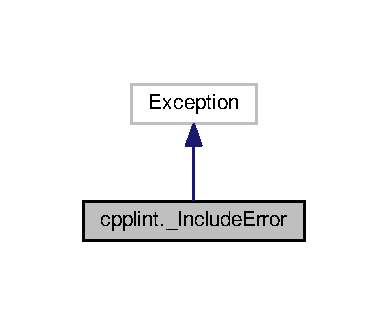
\includegraphics[width=186pt]{classcpplint_1_1__IncludeError__inherit__graph}
\end{center}
\end{figure}


Collaboration diagram for cpplint.\+\_\+\+Include\+Error\+:\nopagebreak
\begin{figure}[H]
\begin{center}
\leavevmode
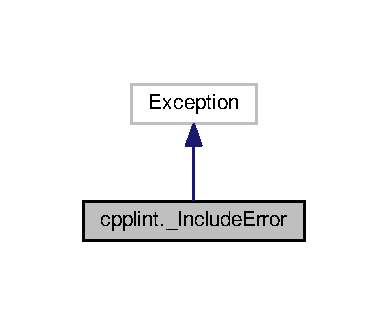
\includegraphics[width=186pt]{classcpplint_1_1__IncludeError__coll__graph}
\end{center}
\end{figure}


\subsection{Detailed Description}
\begin{DoxyVerb}Indicates a problem with the include order in a file.\end{DoxyVerb}
 

The documentation for this class was generated from the following file\+:\begin{DoxyCompactItemize}
\item 
\hyperlink{cpplint_8py}{cpplint.\+py}\end{DoxyCompactItemize}

\hypertarget{classcpplint_1_1__IncludeState}{}\section{cpplint.\+\_\+\+Include\+State Class Reference}
\label{classcpplint_1_1__IncludeState}\index{cpplint.\+\_\+\+Include\+State@{cpplint.\+\_\+\+Include\+State}}


Inheritance diagram for cpplint.\+\_\+\+Include\+State\+:\nopagebreak
\begin{figure}[H]
\begin{center}
\leavevmode
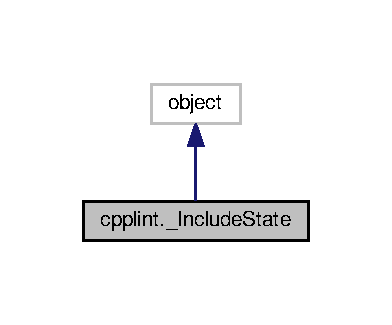
\includegraphics[width=188pt]{classcpplint_1_1__IncludeState__inherit__graph}
\end{center}
\end{figure}


Collaboration diagram for cpplint.\+\_\+\+Include\+State\+:\nopagebreak
\begin{figure}[H]
\begin{center}
\leavevmode
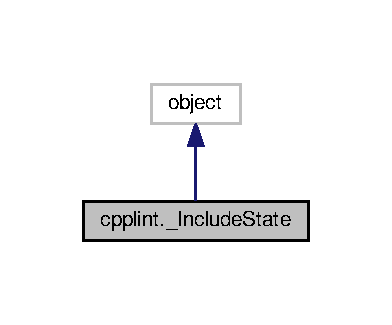
\includegraphics[width=188pt]{classcpplint_1_1__IncludeState__coll__graph}
\end{center}
\end{figure}
\subsection*{Public Member Functions}
\begin{DoxyCompactItemize}
\item 
def \hyperlink{classcpplint_1_1__IncludeState_a4d3ae4ee2a38efc25cce07e3e8484ba4}{\+\_\+\+\_\+init\+\_\+\+\_\+} (self)
\item 
def \hyperlink{classcpplint_1_1__IncludeState_a9bddbf581fc7a4c3c0258eaa42b94c3a}{Find\+Header} (self, header)
\item 
def \hyperlink{classcpplint_1_1__IncludeState_a31551f83fcc626e7babb1581a486b6fa}{Reset\+Section} (self, directive)
\item 
def \hyperlink{classcpplint_1_1__IncludeState_a9bc1ada2060a49628c1fffa973b57df1}{Set\+Last\+Header} (self, header\+\_\+path)
\item 
def \hyperlink{classcpplint_1_1__IncludeState_ae69c652befa2d160194c0a02ff0c7d48}{Canonicalize\+Alphabetical\+Order} (self, header\+\_\+path)
\item 
def \hyperlink{classcpplint_1_1__IncludeState_abfda27324121ab0bf9d29866d975274b}{Is\+In\+Alphabetical\+Order} (self, clean\+\_\+lines, linenum, header\+\_\+path)
\item 
def \hyperlink{classcpplint_1_1__IncludeState_a80f82f17565e8412e7e5bbe52b464f18}{Check\+Next\+Include\+Order} (self, header\+\_\+type)
\end{DoxyCompactItemize}
\subsection*{Public Attributes}
\begin{DoxyCompactItemize}
\item 
\hyperlink{classcpplint_1_1__IncludeState_a82d8b92a431437ee181e950517c71cbb}{include\+\_\+list}
\end{DoxyCompactItemize}


\subsection{Detailed Description}
\begin{DoxyVerb}Tracks line numbers for includes, and the order in which includes appear.

include_list contains list of lists of (header, line number) pairs.
It's a lists of lists rather than just one flat list to make it
easier to update across preprocessor boundaries.

Call CheckNextIncludeOrder() once for each header in the file, passing
in the type constants defined above. Calls in an illegal order will
raise an _IncludeError with an appropriate error message.\end{DoxyVerb}
 

\subsection{Constructor \& Destructor Documentation}
\index{cpplint\+::\+\_\+\+Include\+State@{cpplint\+::\+\_\+\+Include\+State}!\+\_\+\+\_\+init\+\_\+\+\_\+@{\+\_\+\+\_\+init\+\_\+\+\_\+}}
\index{\+\_\+\+\_\+init\+\_\+\+\_\+@{\+\_\+\+\_\+init\+\_\+\+\_\+}!cpplint\+::\+\_\+\+Include\+State@{cpplint\+::\+\_\+\+Include\+State}}
\subsubsection[{\texorpdfstring{\+\_\+\+\_\+init\+\_\+\+\_\+(self)}{__init__(self)}}]{\setlength{\rightskip}{0pt plus 5cm}def cpplint.\+\_\+\+Include\+State.\+\_\+\+\_\+init\+\_\+\+\_\+ (
\begin{DoxyParamCaption}
\item[{}]{self}
\end{DoxyParamCaption}
)}\hypertarget{classcpplint_1_1__IncludeState_a4d3ae4ee2a38efc25cce07e3e8484ba4}{}\label{classcpplint_1_1__IncludeState_a4d3ae4ee2a38efc25cce07e3e8484ba4}


\subsection{Member Function Documentation}
\index{cpplint\+::\+\_\+\+Include\+State@{cpplint\+::\+\_\+\+Include\+State}!Canonicalize\+Alphabetical\+Order@{Canonicalize\+Alphabetical\+Order}}
\index{Canonicalize\+Alphabetical\+Order@{Canonicalize\+Alphabetical\+Order}!cpplint\+::\+\_\+\+Include\+State@{cpplint\+::\+\_\+\+Include\+State}}
\subsubsection[{\texorpdfstring{Canonicalize\+Alphabetical\+Order(self, header\+\_\+path)}{CanonicalizeAlphabeticalOrder(self, header_path)}}]{\setlength{\rightskip}{0pt plus 5cm}def cpplint.\+\_\+\+Include\+State.\+Canonicalize\+Alphabetical\+Order (
\begin{DoxyParamCaption}
\item[{}]{self, }
\item[{}]{header\+\_\+path}
\end{DoxyParamCaption}
)}\hypertarget{classcpplint_1_1__IncludeState_ae69c652befa2d160194c0a02ff0c7d48}{}\label{classcpplint_1_1__IncludeState_ae69c652befa2d160194c0a02ff0c7d48}
\begin{DoxyVerb}Returns a path canonicalized for alphabetical comparison.

- replaces "-" with "_" so they both cmp the same.
- removes '-inl' since we don't require them to be after the main header.
- lowercase everything, just in case.

Args:
  header_path: Path to be canonicalized.

Returns:
  Canonicalized path.
\end{DoxyVerb}
 \index{cpplint\+::\+\_\+\+Include\+State@{cpplint\+::\+\_\+\+Include\+State}!Check\+Next\+Include\+Order@{Check\+Next\+Include\+Order}}
\index{Check\+Next\+Include\+Order@{Check\+Next\+Include\+Order}!cpplint\+::\+\_\+\+Include\+State@{cpplint\+::\+\_\+\+Include\+State}}
\subsubsection[{\texorpdfstring{Check\+Next\+Include\+Order(self, header\+\_\+type)}{CheckNextIncludeOrder(self, header_type)}}]{\setlength{\rightskip}{0pt plus 5cm}def cpplint.\+\_\+\+Include\+State.\+Check\+Next\+Include\+Order (
\begin{DoxyParamCaption}
\item[{}]{self, }
\item[{}]{header\+\_\+type}
\end{DoxyParamCaption}
)}\hypertarget{classcpplint_1_1__IncludeState_a80f82f17565e8412e7e5bbe52b464f18}{}\label{classcpplint_1_1__IncludeState_a80f82f17565e8412e7e5bbe52b464f18}
\begin{DoxyVerb}Returns a non-empty error message if the next header is out of order.

This function also updates the internal state to be ready to check
the next include.

Args:
  header_type: One of the _XXX_HEADER constants defined above.

Returns:
  The empty string if the header is in the right order, or an
  error message describing what's wrong.\end{DoxyVerb}
 \index{cpplint\+::\+\_\+\+Include\+State@{cpplint\+::\+\_\+\+Include\+State}!Find\+Header@{Find\+Header}}
\index{Find\+Header@{Find\+Header}!cpplint\+::\+\_\+\+Include\+State@{cpplint\+::\+\_\+\+Include\+State}}
\subsubsection[{\texorpdfstring{Find\+Header(self, header)}{FindHeader(self, header)}}]{\setlength{\rightskip}{0pt plus 5cm}def cpplint.\+\_\+\+Include\+State.\+Find\+Header (
\begin{DoxyParamCaption}
\item[{}]{self, }
\item[{}]{header}
\end{DoxyParamCaption}
)}\hypertarget{classcpplint_1_1__IncludeState_a9bddbf581fc7a4c3c0258eaa42b94c3a}{}\label{classcpplint_1_1__IncludeState_a9bddbf581fc7a4c3c0258eaa42b94c3a}
\begin{DoxyVerb}Check if a header has already been included.

Args:
  header: header to check.
Returns:
  Line number of previous occurrence, or -1 if the header has not
  been seen before.
\end{DoxyVerb}
 \index{cpplint\+::\+\_\+\+Include\+State@{cpplint\+::\+\_\+\+Include\+State}!Is\+In\+Alphabetical\+Order@{Is\+In\+Alphabetical\+Order}}
\index{Is\+In\+Alphabetical\+Order@{Is\+In\+Alphabetical\+Order}!cpplint\+::\+\_\+\+Include\+State@{cpplint\+::\+\_\+\+Include\+State}}
\subsubsection[{\texorpdfstring{Is\+In\+Alphabetical\+Order(self, clean\+\_\+lines, linenum, header\+\_\+path)}{IsInAlphabeticalOrder(self, clean_lines, linenum, header_path)}}]{\setlength{\rightskip}{0pt plus 5cm}def cpplint.\+\_\+\+Include\+State.\+Is\+In\+Alphabetical\+Order (
\begin{DoxyParamCaption}
\item[{}]{self, }
\item[{}]{clean\+\_\+lines, }
\item[{}]{linenum, }
\item[{}]{header\+\_\+path}
\end{DoxyParamCaption}
)}\hypertarget{classcpplint_1_1__IncludeState_abfda27324121ab0bf9d29866d975274b}{}\label{classcpplint_1_1__IncludeState_abfda27324121ab0bf9d29866d975274b}
\begin{DoxyVerb}Check if a header is in alphabetical order with the previous header.

Args:
  clean_lines: A CleansedLines instance containing the file.
  linenum: The number of the line to check.
  header_path: Canonicalized header to be checked.

Returns:
  Returns true if the header is in alphabetical order.
\end{DoxyVerb}
 \index{cpplint\+::\+\_\+\+Include\+State@{cpplint\+::\+\_\+\+Include\+State}!Reset\+Section@{Reset\+Section}}
\index{Reset\+Section@{Reset\+Section}!cpplint\+::\+\_\+\+Include\+State@{cpplint\+::\+\_\+\+Include\+State}}
\subsubsection[{\texorpdfstring{Reset\+Section(self, directive)}{ResetSection(self, directive)}}]{\setlength{\rightskip}{0pt plus 5cm}def cpplint.\+\_\+\+Include\+State.\+Reset\+Section (
\begin{DoxyParamCaption}
\item[{}]{self, }
\item[{}]{directive}
\end{DoxyParamCaption}
)}\hypertarget{classcpplint_1_1__IncludeState_a31551f83fcc626e7babb1581a486b6fa}{}\label{classcpplint_1_1__IncludeState_a31551f83fcc626e7babb1581a486b6fa}
\begin{DoxyVerb}Reset section checking for preprocessor directive.

Args:
  directive: preprocessor directive (e.g. "if", "else").
\end{DoxyVerb}
 \index{cpplint\+::\+\_\+\+Include\+State@{cpplint\+::\+\_\+\+Include\+State}!Set\+Last\+Header@{Set\+Last\+Header}}
\index{Set\+Last\+Header@{Set\+Last\+Header}!cpplint\+::\+\_\+\+Include\+State@{cpplint\+::\+\_\+\+Include\+State}}
\subsubsection[{\texorpdfstring{Set\+Last\+Header(self, header\+\_\+path)}{SetLastHeader(self, header_path)}}]{\setlength{\rightskip}{0pt plus 5cm}def cpplint.\+\_\+\+Include\+State.\+Set\+Last\+Header (
\begin{DoxyParamCaption}
\item[{}]{self, }
\item[{}]{header\+\_\+path}
\end{DoxyParamCaption}
)}\hypertarget{classcpplint_1_1__IncludeState_a9bc1ada2060a49628c1fffa973b57df1}{}\label{classcpplint_1_1__IncludeState_a9bc1ada2060a49628c1fffa973b57df1}


\subsection{Member Data Documentation}
\index{cpplint\+::\+\_\+\+Include\+State@{cpplint\+::\+\_\+\+Include\+State}!include\+\_\+list@{include\+\_\+list}}
\index{include\+\_\+list@{include\+\_\+list}!cpplint\+::\+\_\+\+Include\+State@{cpplint\+::\+\_\+\+Include\+State}}
\subsubsection[{\texorpdfstring{include\+\_\+list}{include_list}}]{\setlength{\rightskip}{0pt plus 5cm}cpplint.\+\_\+\+Include\+State.\+include\+\_\+list}\hypertarget{classcpplint_1_1__IncludeState_a82d8b92a431437ee181e950517c71cbb}{}\label{classcpplint_1_1__IncludeState_a82d8b92a431437ee181e950517c71cbb}


The documentation for this class was generated from the following file\+:\begin{DoxyCompactItemize}
\item 
\hyperlink{cpplint_8py}{cpplint.\+py}\end{DoxyCompactItemize}

\hypertarget{classcpplint_1_1__NamespaceInfo}{}\section{cpplint.\+\_\+\+Namespace\+Info Class Reference}
\label{classcpplint_1_1__NamespaceInfo}\index{cpplint.\+\_\+\+Namespace\+Info@{cpplint.\+\_\+\+Namespace\+Info}}


Inheritance diagram for cpplint.\+\_\+\+Namespace\+Info\+:\nopagebreak
\begin{figure}[H]
\begin{center}
\leavevmode
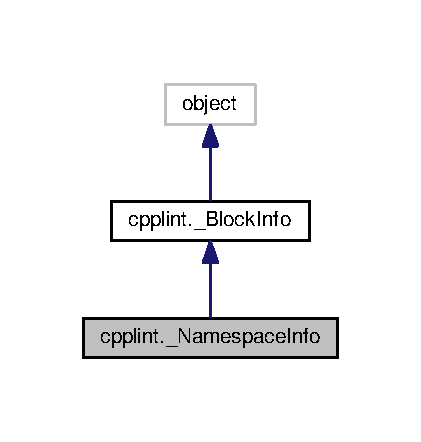
\includegraphics[width=202pt]{classcpplint_1_1__NamespaceInfo__inherit__graph}
\end{center}
\end{figure}


Collaboration diagram for cpplint.\+\_\+\+Namespace\+Info\+:\nopagebreak
\begin{figure}[H]
\begin{center}
\leavevmode
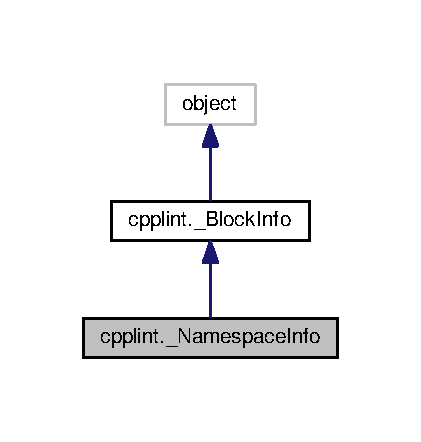
\includegraphics[width=202pt]{classcpplint_1_1__NamespaceInfo__coll__graph}
\end{center}
\end{figure}
\subsection*{Public Member Functions}
\begin{DoxyCompactItemize}
\item 
def \hyperlink{classcpplint_1_1__NamespaceInfo_a4425c93bd90fbf869dc31c87302f5bb0}{\+\_\+\+\_\+init\+\_\+\+\_\+} (self, \hyperlink{classcpplint_1_1__NamespaceInfo_a6b518dae822e4e440405654e83dc86a1}{name}, linenum)
\item 
def \hyperlink{classcpplint_1_1__NamespaceInfo_a9d3abaeed0353942ca689eeeb2f2924b}{Check\+End} (self, filename, clean\+\_\+lines, linenum, error)
\end{DoxyCompactItemize}
\subsection*{Public Attributes}
\begin{DoxyCompactItemize}
\item 
\hyperlink{classcpplint_1_1__NamespaceInfo_a6b518dae822e4e440405654e83dc86a1}{name}
\item 
\hyperlink{classcpplint_1_1__NamespaceInfo_ae0b0b6ffafd3336a93cddca1078df268}{check\+\_\+namespace\+\_\+indentation}
\end{DoxyCompactItemize}


\subsection{Detailed Description}
\begin{DoxyVerb}Stores information about a namespace.\end{DoxyVerb}
 

\subsection{Constructor \& Destructor Documentation}
\index{cpplint\+::\+\_\+\+Namespace\+Info@{cpplint\+::\+\_\+\+Namespace\+Info}!\+\_\+\+\_\+init\+\_\+\+\_\+@{\+\_\+\+\_\+init\+\_\+\+\_\+}}
\index{\+\_\+\+\_\+init\+\_\+\+\_\+@{\+\_\+\+\_\+init\+\_\+\+\_\+}!cpplint\+::\+\_\+\+Namespace\+Info@{cpplint\+::\+\_\+\+Namespace\+Info}}
\subsubsection[{\texorpdfstring{\+\_\+\+\_\+init\+\_\+\+\_\+(self, name, linenum)}{__init__(self, name, linenum)}}]{\setlength{\rightskip}{0pt plus 5cm}def cpplint.\+\_\+\+Namespace\+Info.\+\_\+\+\_\+init\+\_\+\+\_\+ (
\begin{DoxyParamCaption}
\item[{}]{self, }
\item[{}]{name, }
\item[{}]{linenum}
\end{DoxyParamCaption}
)}\hypertarget{classcpplint_1_1__NamespaceInfo_a4425c93bd90fbf869dc31c87302f5bb0}{}\label{classcpplint_1_1__NamespaceInfo_a4425c93bd90fbf869dc31c87302f5bb0}


\subsection{Member Function Documentation}
\index{cpplint\+::\+\_\+\+Namespace\+Info@{cpplint\+::\+\_\+\+Namespace\+Info}!Check\+End@{Check\+End}}
\index{Check\+End@{Check\+End}!cpplint\+::\+\_\+\+Namespace\+Info@{cpplint\+::\+\_\+\+Namespace\+Info}}
\subsubsection[{\texorpdfstring{Check\+End(self, filename, clean\+\_\+lines, linenum, error)}{CheckEnd(self, filename, clean_lines, linenum, error)}}]{\setlength{\rightskip}{0pt plus 5cm}def cpplint.\+\_\+\+Namespace\+Info.\+Check\+End (
\begin{DoxyParamCaption}
\item[{}]{self, }
\item[{}]{filename, }
\item[{}]{clean\+\_\+lines, }
\item[{}]{linenum, }
\item[{}]{error}
\end{DoxyParamCaption}
)}\hypertarget{classcpplint_1_1__NamespaceInfo_a9d3abaeed0353942ca689eeeb2f2924b}{}\label{classcpplint_1_1__NamespaceInfo_a9d3abaeed0353942ca689eeeb2f2924b}
\begin{DoxyVerb}Check end of namespace comments.\end{DoxyVerb}
 

\subsection{Member Data Documentation}
\index{cpplint\+::\+\_\+\+Namespace\+Info@{cpplint\+::\+\_\+\+Namespace\+Info}!check\+\_\+namespace\+\_\+indentation@{check\+\_\+namespace\+\_\+indentation}}
\index{check\+\_\+namespace\+\_\+indentation@{check\+\_\+namespace\+\_\+indentation}!cpplint\+::\+\_\+\+Namespace\+Info@{cpplint\+::\+\_\+\+Namespace\+Info}}
\subsubsection[{\texorpdfstring{check\+\_\+namespace\+\_\+indentation}{check_namespace_indentation}}]{\setlength{\rightskip}{0pt plus 5cm}cpplint.\+\_\+\+Namespace\+Info.\+check\+\_\+namespace\+\_\+indentation}\hypertarget{classcpplint_1_1__NamespaceInfo_ae0b0b6ffafd3336a93cddca1078df268}{}\label{classcpplint_1_1__NamespaceInfo_ae0b0b6ffafd3336a93cddca1078df268}
\index{cpplint\+::\+\_\+\+Namespace\+Info@{cpplint\+::\+\_\+\+Namespace\+Info}!name@{name}}
\index{name@{name}!cpplint\+::\+\_\+\+Namespace\+Info@{cpplint\+::\+\_\+\+Namespace\+Info}}
\subsubsection[{\texorpdfstring{name}{name}}]{\setlength{\rightskip}{0pt plus 5cm}cpplint.\+\_\+\+Namespace\+Info.\+name}\hypertarget{classcpplint_1_1__NamespaceInfo_a6b518dae822e4e440405654e83dc86a1}{}\label{classcpplint_1_1__NamespaceInfo_a6b518dae822e4e440405654e83dc86a1}


The documentation for this class was generated from the following file\+:\begin{DoxyCompactItemize}
\item 
\hyperlink{cpplint_8py}{cpplint.\+py}\end{DoxyCompactItemize}

\hypertarget{classcpplint_1_1__PreprocessorInfo}{}\section{cpplint.\+\_\+\+Preprocessor\+Info Class Reference}
\label{classcpplint_1_1__PreprocessorInfo}\index{cpplint.\+\_\+\+Preprocessor\+Info@{cpplint.\+\_\+\+Preprocessor\+Info}}


Inheritance diagram for cpplint.\+\_\+\+Preprocessor\+Info\+:\nopagebreak
\begin{figure}[H]
\begin{center}
\leavevmode
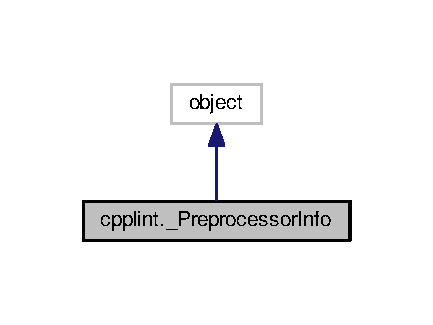
\includegraphics[width=208pt]{classcpplint_1_1__PreprocessorInfo__inherit__graph}
\end{center}
\end{figure}


Collaboration diagram for cpplint.\+\_\+\+Preprocessor\+Info\+:\nopagebreak
\begin{figure}[H]
\begin{center}
\leavevmode
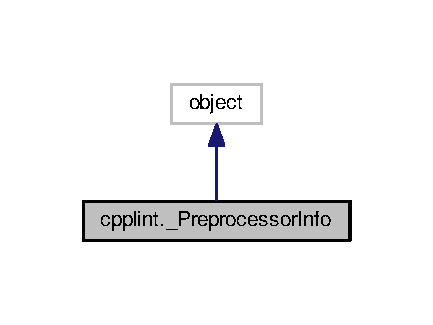
\includegraphics[width=208pt]{classcpplint_1_1__PreprocessorInfo__coll__graph}
\end{center}
\end{figure}
\subsection*{Public Member Functions}
\begin{DoxyCompactItemize}
\item 
def \hyperlink{classcpplint_1_1__PreprocessorInfo_a1394d17434a22d32b0ea9d6424e5c47b}{\+\_\+\+\_\+init\+\_\+\+\_\+} (self, \hyperlink{classcpplint_1_1__PreprocessorInfo_a0681b2adca3171a495fc1eca43d245c0}{stack\+\_\+before\+\_\+if})
\end{DoxyCompactItemize}
\subsection*{Public Attributes}
\begin{DoxyCompactItemize}
\item 
\hyperlink{classcpplint_1_1__PreprocessorInfo_a0681b2adca3171a495fc1eca43d245c0}{stack\+\_\+before\+\_\+if}
\item 
\hyperlink{classcpplint_1_1__PreprocessorInfo_a34a80f1f97808614b7062ba1e5bbf2b9}{stack\+\_\+before\+\_\+else}
\item 
\hyperlink{classcpplint_1_1__PreprocessorInfo_a7587e84a1e6db34c3c94317f5a5931cc}{seen\+\_\+else}
\end{DoxyCompactItemize}


\subsection{Detailed Description}
\begin{DoxyVerb}Stores checkpoints of nesting stacks when #if/#else is seen.\end{DoxyVerb}
 

\subsection{Constructor \& Destructor Documentation}
\index{cpplint\+::\+\_\+\+Preprocessor\+Info@{cpplint\+::\+\_\+\+Preprocessor\+Info}!\+\_\+\+\_\+init\+\_\+\+\_\+@{\+\_\+\+\_\+init\+\_\+\+\_\+}}
\index{\+\_\+\+\_\+init\+\_\+\+\_\+@{\+\_\+\+\_\+init\+\_\+\+\_\+}!cpplint\+::\+\_\+\+Preprocessor\+Info@{cpplint\+::\+\_\+\+Preprocessor\+Info}}
\subsubsection[{\texorpdfstring{\+\_\+\+\_\+init\+\_\+\+\_\+(self, stack\+\_\+before\+\_\+if)}{__init__(self, stack_before_if)}}]{\setlength{\rightskip}{0pt plus 5cm}def cpplint.\+\_\+\+Preprocessor\+Info.\+\_\+\+\_\+init\+\_\+\+\_\+ (
\begin{DoxyParamCaption}
\item[{}]{self, }
\item[{}]{stack\+\_\+before\+\_\+if}
\end{DoxyParamCaption}
)}\hypertarget{classcpplint_1_1__PreprocessorInfo_a1394d17434a22d32b0ea9d6424e5c47b}{}\label{classcpplint_1_1__PreprocessorInfo_a1394d17434a22d32b0ea9d6424e5c47b}


\subsection{Member Data Documentation}
\index{cpplint\+::\+\_\+\+Preprocessor\+Info@{cpplint\+::\+\_\+\+Preprocessor\+Info}!seen\+\_\+else@{seen\+\_\+else}}
\index{seen\+\_\+else@{seen\+\_\+else}!cpplint\+::\+\_\+\+Preprocessor\+Info@{cpplint\+::\+\_\+\+Preprocessor\+Info}}
\subsubsection[{\texorpdfstring{seen\+\_\+else}{seen_else}}]{\setlength{\rightskip}{0pt plus 5cm}cpplint.\+\_\+\+Preprocessor\+Info.\+seen\+\_\+else}\hypertarget{classcpplint_1_1__PreprocessorInfo_a7587e84a1e6db34c3c94317f5a5931cc}{}\label{classcpplint_1_1__PreprocessorInfo_a7587e84a1e6db34c3c94317f5a5931cc}
\index{cpplint\+::\+\_\+\+Preprocessor\+Info@{cpplint\+::\+\_\+\+Preprocessor\+Info}!stack\+\_\+before\+\_\+else@{stack\+\_\+before\+\_\+else}}
\index{stack\+\_\+before\+\_\+else@{stack\+\_\+before\+\_\+else}!cpplint\+::\+\_\+\+Preprocessor\+Info@{cpplint\+::\+\_\+\+Preprocessor\+Info}}
\subsubsection[{\texorpdfstring{stack\+\_\+before\+\_\+else}{stack_before_else}}]{\setlength{\rightskip}{0pt plus 5cm}cpplint.\+\_\+\+Preprocessor\+Info.\+stack\+\_\+before\+\_\+else}\hypertarget{classcpplint_1_1__PreprocessorInfo_a34a80f1f97808614b7062ba1e5bbf2b9}{}\label{classcpplint_1_1__PreprocessorInfo_a34a80f1f97808614b7062ba1e5bbf2b9}
\index{cpplint\+::\+\_\+\+Preprocessor\+Info@{cpplint\+::\+\_\+\+Preprocessor\+Info}!stack\+\_\+before\+\_\+if@{stack\+\_\+before\+\_\+if}}
\index{stack\+\_\+before\+\_\+if@{stack\+\_\+before\+\_\+if}!cpplint\+::\+\_\+\+Preprocessor\+Info@{cpplint\+::\+\_\+\+Preprocessor\+Info}}
\subsubsection[{\texorpdfstring{stack\+\_\+before\+\_\+if}{stack_before_if}}]{\setlength{\rightskip}{0pt plus 5cm}cpplint.\+\_\+\+Preprocessor\+Info.\+stack\+\_\+before\+\_\+if}\hypertarget{classcpplint_1_1__PreprocessorInfo_a0681b2adca3171a495fc1eca43d245c0}{}\label{classcpplint_1_1__PreprocessorInfo_a0681b2adca3171a495fc1eca43d245c0}


The documentation for this class was generated from the following file\+:\begin{DoxyCompactItemize}
\item 
\hyperlink{cpplint_8py}{cpplint.\+py}\end{DoxyCompactItemize}

\hypertarget{classcpplint_1_1CleansedLines}{}\section{cpplint.\+Cleansed\+Lines Class Reference}
\label{classcpplint_1_1CleansedLines}\index{cpplint.\+Cleansed\+Lines@{cpplint.\+Cleansed\+Lines}}


Inheritance diagram for cpplint.\+Cleansed\+Lines\+:\nopagebreak
\begin{figure}[H]
\begin{center}
\leavevmode
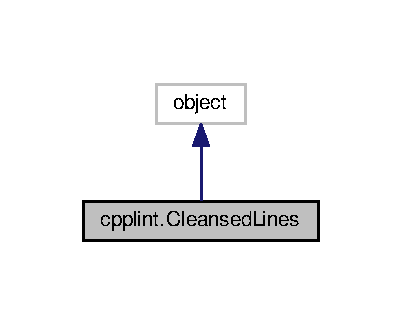
\includegraphics[width=193pt]{classcpplint_1_1CleansedLines__inherit__graph}
\end{center}
\end{figure}


Collaboration diagram for cpplint.\+Cleansed\+Lines\+:\nopagebreak
\begin{figure}[H]
\begin{center}
\leavevmode
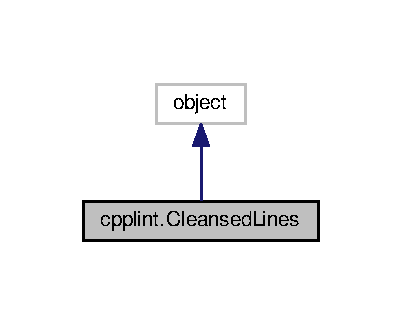
\includegraphics[width=193pt]{classcpplint_1_1CleansedLines__coll__graph}
\end{center}
\end{figure}
\subsection*{Public Member Functions}
\begin{DoxyCompactItemize}
\item 
def \hyperlink{classcpplint_1_1CleansedLines_ad2bc06d9697e2bbfbc7e6b50878c8c8f}{\+\_\+\+\_\+init\+\_\+\+\_\+} (self, \hyperlink{classcpplint_1_1CleansedLines_a9cd74bd010da1610a46322d6821bd06a}{lines})
\item 
def \hyperlink{classcpplint_1_1CleansedLines_a26a7eff70493d64d58d16f4a406c7ee9}{Num\+Lines} (self)
\end{DoxyCompactItemize}
\subsection*{Public Attributes}
\begin{DoxyCompactItemize}
\item 
\hyperlink{classcpplint_1_1CleansedLines_aa4d0a4d5081675c01656a5d86d99e8bd}{elided}
\item 
\hyperlink{classcpplint_1_1CleansedLines_a9cd74bd010da1610a46322d6821bd06a}{lines}
\item 
\hyperlink{classcpplint_1_1CleansedLines_a9e94ce9e4f682be33c04fe82429c4dfd}{raw\+\_\+lines}
\item 
\hyperlink{classcpplint_1_1CleansedLines_a4b42ab48659954fb6e0a4e4eb483a45a}{num\+\_\+lines}
\item 
\hyperlink{classcpplint_1_1CleansedLines_a0cc228ba3c00ba590b27a759cf8023ce}{lines\+\_\+without\+\_\+raw\+\_\+strings}
\end{DoxyCompactItemize}


\subsection{Detailed Description}
\begin{DoxyVerb}Holds 4 copies of all lines with different preprocessing applied to them.

1) elided member contains lines without strings and comments.
2) lines member contains lines without comments.
3) raw_lines member contains all the lines without processing.
4) lines_without_raw_strings member is same as raw_lines, but with C++11 raw
   strings removed.
All these members are of <type 'list'>, and of the same length.
\end{DoxyVerb}
 

\subsection{Constructor \& Destructor Documentation}
\index{cpplint\+::\+Cleansed\+Lines@{cpplint\+::\+Cleansed\+Lines}!\+\_\+\+\_\+init\+\_\+\+\_\+@{\+\_\+\+\_\+init\+\_\+\+\_\+}}
\index{\+\_\+\+\_\+init\+\_\+\+\_\+@{\+\_\+\+\_\+init\+\_\+\+\_\+}!cpplint\+::\+Cleansed\+Lines@{cpplint\+::\+Cleansed\+Lines}}
\subsubsection[{\texorpdfstring{\+\_\+\+\_\+init\+\_\+\+\_\+(self, lines)}{__init__(self, lines)}}]{\setlength{\rightskip}{0pt plus 5cm}def cpplint.\+Cleansed\+Lines.\+\_\+\+\_\+init\+\_\+\+\_\+ (
\begin{DoxyParamCaption}
\item[{}]{self, }
\item[{}]{lines}
\end{DoxyParamCaption}
)}\hypertarget{classcpplint_1_1CleansedLines_ad2bc06d9697e2bbfbc7e6b50878c8c8f}{}\label{classcpplint_1_1CleansedLines_ad2bc06d9697e2bbfbc7e6b50878c8c8f}


\subsection{Member Function Documentation}
\index{cpplint\+::\+Cleansed\+Lines@{cpplint\+::\+Cleansed\+Lines}!Num\+Lines@{Num\+Lines}}
\index{Num\+Lines@{Num\+Lines}!cpplint\+::\+Cleansed\+Lines@{cpplint\+::\+Cleansed\+Lines}}
\subsubsection[{\texorpdfstring{Num\+Lines(self)}{NumLines(self)}}]{\setlength{\rightskip}{0pt plus 5cm}def cpplint.\+Cleansed\+Lines.\+Num\+Lines (
\begin{DoxyParamCaption}
\item[{}]{self}
\end{DoxyParamCaption}
)}\hypertarget{classcpplint_1_1CleansedLines_a26a7eff70493d64d58d16f4a406c7ee9}{}\label{classcpplint_1_1CleansedLines_a26a7eff70493d64d58d16f4a406c7ee9}
\begin{DoxyVerb}Returns the number of lines represented.\end{DoxyVerb}
 

\subsection{Member Data Documentation}
\index{cpplint\+::\+Cleansed\+Lines@{cpplint\+::\+Cleansed\+Lines}!elided@{elided}}
\index{elided@{elided}!cpplint\+::\+Cleansed\+Lines@{cpplint\+::\+Cleansed\+Lines}}
\subsubsection[{\texorpdfstring{elided}{elided}}]{\setlength{\rightskip}{0pt plus 5cm}cpplint.\+Cleansed\+Lines.\+elided}\hypertarget{classcpplint_1_1CleansedLines_aa4d0a4d5081675c01656a5d86d99e8bd}{}\label{classcpplint_1_1CleansedLines_aa4d0a4d5081675c01656a5d86d99e8bd}
\index{cpplint\+::\+Cleansed\+Lines@{cpplint\+::\+Cleansed\+Lines}!lines@{lines}}
\index{lines@{lines}!cpplint\+::\+Cleansed\+Lines@{cpplint\+::\+Cleansed\+Lines}}
\subsubsection[{\texorpdfstring{lines}{lines}}]{\setlength{\rightskip}{0pt plus 5cm}cpplint.\+Cleansed\+Lines.\+lines}\hypertarget{classcpplint_1_1CleansedLines_a9cd74bd010da1610a46322d6821bd06a}{}\label{classcpplint_1_1CleansedLines_a9cd74bd010da1610a46322d6821bd06a}
\index{cpplint\+::\+Cleansed\+Lines@{cpplint\+::\+Cleansed\+Lines}!lines\+\_\+without\+\_\+raw\+\_\+strings@{lines\+\_\+without\+\_\+raw\+\_\+strings}}
\index{lines\+\_\+without\+\_\+raw\+\_\+strings@{lines\+\_\+without\+\_\+raw\+\_\+strings}!cpplint\+::\+Cleansed\+Lines@{cpplint\+::\+Cleansed\+Lines}}
\subsubsection[{\texorpdfstring{lines\+\_\+without\+\_\+raw\+\_\+strings}{lines_without_raw_strings}}]{\setlength{\rightskip}{0pt plus 5cm}cpplint.\+Cleansed\+Lines.\+lines\+\_\+without\+\_\+raw\+\_\+strings}\hypertarget{classcpplint_1_1CleansedLines_a0cc228ba3c00ba590b27a759cf8023ce}{}\label{classcpplint_1_1CleansedLines_a0cc228ba3c00ba590b27a759cf8023ce}
\index{cpplint\+::\+Cleansed\+Lines@{cpplint\+::\+Cleansed\+Lines}!num\+\_\+lines@{num\+\_\+lines}}
\index{num\+\_\+lines@{num\+\_\+lines}!cpplint\+::\+Cleansed\+Lines@{cpplint\+::\+Cleansed\+Lines}}
\subsubsection[{\texorpdfstring{num\+\_\+lines}{num_lines}}]{\setlength{\rightskip}{0pt plus 5cm}cpplint.\+Cleansed\+Lines.\+num\+\_\+lines}\hypertarget{classcpplint_1_1CleansedLines_a4b42ab48659954fb6e0a4e4eb483a45a}{}\label{classcpplint_1_1CleansedLines_a4b42ab48659954fb6e0a4e4eb483a45a}
\index{cpplint\+::\+Cleansed\+Lines@{cpplint\+::\+Cleansed\+Lines}!raw\+\_\+lines@{raw\+\_\+lines}}
\index{raw\+\_\+lines@{raw\+\_\+lines}!cpplint\+::\+Cleansed\+Lines@{cpplint\+::\+Cleansed\+Lines}}
\subsubsection[{\texorpdfstring{raw\+\_\+lines}{raw_lines}}]{\setlength{\rightskip}{0pt plus 5cm}cpplint.\+Cleansed\+Lines.\+raw\+\_\+lines}\hypertarget{classcpplint_1_1CleansedLines_a9e94ce9e4f682be33c04fe82429c4dfd}{}\label{classcpplint_1_1CleansedLines_a9e94ce9e4f682be33c04fe82429c4dfd}


The documentation for this class was generated from the following file\+:\begin{DoxyCompactItemize}
\item 
\hyperlink{cpplint_8py}{cpplint.\+py}\end{DoxyCompactItemize}

\hypertarget{classcpplint_1_1FileInfo}{}\section{cpplint.\+File\+Info Class Reference}
\label{classcpplint_1_1FileInfo}\index{cpplint.\+File\+Info@{cpplint.\+File\+Info}}


Inheritance diagram for cpplint.\+File\+Info\+:\nopagebreak
\begin{figure}[H]
\begin{center}
\leavevmode
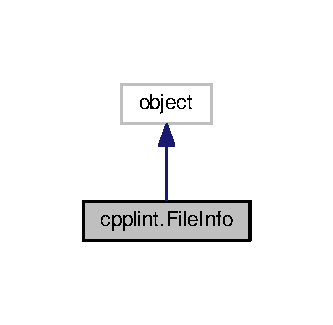
\includegraphics[width=160pt]{classcpplint_1_1FileInfo__inherit__graph}
\end{center}
\end{figure}


Collaboration diagram for cpplint.\+File\+Info\+:\nopagebreak
\begin{figure}[H]
\begin{center}
\leavevmode
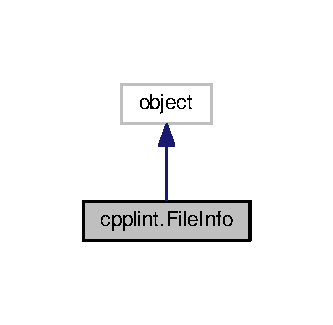
\includegraphics[width=160pt]{classcpplint_1_1FileInfo__coll__graph}
\end{center}
\end{figure}
\subsection*{Public Member Functions}
\begin{DoxyCompactItemize}
\item 
def \hyperlink{classcpplint_1_1FileInfo_abd3ff77aab027af2476b3a1d97b1f89c}{\+\_\+\+\_\+init\+\_\+\+\_\+} (self, filename)
\item 
def \hyperlink{classcpplint_1_1FileInfo_aed56577368c45cdf45fc4c9109129145}{Full\+Name} (self)
\item 
def \hyperlink{classcpplint_1_1FileInfo_a2b3b79b7d46221a6b9d0ea0bebac2061}{Repository\+Name} (self)
\item 
def \hyperlink{classcpplint_1_1FileInfo_a43f1c5ff1771da52e29c60c114955e72}{Split} (self)
\item 
def \hyperlink{classcpplint_1_1FileInfo_a1a12ed63ddc2ffd8f6a105e3ab4d6289}{Base\+Name} (self)
\item 
def \hyperlink{classcpplint_1_1FileInfo_a2554b504117839931e901b59a59c67ae}{Extension} (self)
\item 
def \hyperlink{classcpplint_1_1FileInfo_acb46555a72b346966f4bf28c08e3b1fa}{No\+Extension} (self)
\item 
def \hyperlink{classcpplint_1_1FileInfo_a157f8d3266d7291321db88cdad3b2879}{Is\+Source} (self)
\end{DoxyCompactItemize}


\subsection{Detailed Description}
\begin{DoxyVerb}Provides utility functions for filenames.

FileInfo provides easy access to the components of a file's path
relative to the project root.
\end{DoxyVerb}
 

\subsection{Constructor \& Destructor Documentation}
\index{cpplint\+::\+File\+Info@{cpplint\+::\+File\+Info}!\+\_\+\+\_\+init\+\_\+\+\_\+@{\+\_\+\+\_\+init\+\_\+\+\_\+}}
\index{\+\_\+\+\_\+init\+\_\+\+\_\+@{\+\_\+\+\_\+init\+\_\+\+\_\+}!cpplint\+::\+File\+Info@{cpplint\+::\+File\+Info}}
\subsubsection[{\texorpdfstring{\+\_\+\+\_\+init\+\_\+\+\_\+(self, filename)}{__init__(self, filename)}}]{\setlength{\rightskip}{0pt plus 5cm}def cpplint.\+File\+Info.\+\_\+\+\_\+init\+\_\+\+\_\+ (
\begin{DoxyParamCaption}
\item[{}]{self, }
\item[{}]{filename}
\end{DoxyParamCaption}
)}\hypertarget{classcpplint_1_1FileInfo_abd3ff77aab027af2476b3a1d97b1f89c}{}\label{classcpplint_1_1FileInfo_abd3ff77aab027af2476b3a1d97b1f89c}


\subsection{Member Function Documentation}
\index{cpplint\+::\+File\+Info@{cpplint\+::\+File\+Info}!Base\+Name@{Base\+Name}}
\index{Base\+Name@{Base\+Name}!cpplint\+::\+File\+Info@{cpplint\+::\+File\+Info}}
\subsubsection[{\texorpdfstring{Base\+Name(self)}{BaseName(self)}}]{\setlength{\rightskip}{0pt plus 5cm}def cpplint.\+File\+Info.\+Base\+Name (
\begin{DoxyParamCaption}
\item[{}]{self}
\end{DoxyParamCaption}
)}\hypertarget{classcpplint_1_1FileInfo_a1a12ed63ddc2ffd8f6a105e3ab4d6289}{}\label{classcpplint_1_1FileInfo_a1a12ed63ddc2ffd8f6a105e3ab4d6289}
\begin{DoxyVerb}File base name - text after the final slash, before the final period.\end{DoxyVerb}
 \index{cpplint\+::\+File\+Info@{cpplint\+::\+File\+Info}!Extension@{Extension}}
\index{Extension@{Extension}!cpplint\+::\+File\+Info@{cpplint\+::\+File\+Info}}
\subsubsection[{\texorpdfstring{Extension(self)}{Extension(self)}}]{\setlength{\rightskip}{0pt plus 5cm}def cpplint.\+File\+Info.\+Extension (
\begin{DoxyParamCaption}
\item[{}]{self}
\end{DoxyParamCaption}
)}\hypertarget{classcpplint_1_1FileInfo_a2554b504117839931e901b59a59c67ae}{}\label{classcpplint_1_1FileInfo_a2554b504117839931e901b59a59c67ae}
\begin{DoxyVerb}File extension - text following the final period.\end{DoxyVerb}
 \index{cpplint\+::\+File\+Info@{cpplint\+::\+File\+Info}!Full\+Name@{Full\+Name}}
\index{Full\+Name@{Full\+Name}!cpplint\+::\+File\+Info@{cpplint\+::\+File\+Info}}
\subsubsection[{\texorpdfstring{Full\+Name(self)}{FullName(self)}}]{\setlength{\rightskip}{0pt plus 5cm}def cpplint.\+File\+Info.\+Full\+Name (
\begin{DoxyParamCaption}
\item[{}]{self}
\end{DoxyParamCaption}
)}\hypertarget{classcpplint_1_1FileInfo_aed56577368c45cdf45fc4c9109129145}{}\label{classcpplint_1_1FileInfo_aed56577368c45cdf45fc4c9109129145}
\begin{DoxyVerb}Make Windows paths like Unix.\end{DoxyVerb}
 \index{cpplint\+::\+File\+Info@{cpplint\+::\+File\+Info}!Is\+Source@{Is\+Source}}
\index{Is\+Source@{Is\+Source}!cpplint\+::\+File\+Info@{cpplint\+::\+File\+Info}}
\subsubsection[{\texorpdfstring{Is\+Source(self)}{IsSource(self)}}]{\setlength{\rightskip}{0pt plus 5cm}def cpplint.\+File\+Info.\+Is\+Source (
\begin{DoxyParamCaption}
\item[{}]{self}
\end{DoxyParamCaption}
)}\hypertarget{classcpplint_1_1FileInfo_a157f8d3266d7291321db88cdad3b2879}{}\label{classcpplint_1_1FileInfo_a157f8d3266d7291321db88cdad3b2879}
\begin{DoxyVerb}File has a source file extension.\end{DoxyVerb}
 \index{cpplint\+::\+File\+Info@{cpplint\+::\+File\+Info}!No\+Extension@{No\+Extension}}
\index{No\+Extension@{No\+Extension}!cpplint\+::\+File\+Info@{cpplint\+::\+File\+Info}}
\subsubsection[{\texorpdfstring{No\+Extension(self)}{NoExtension(self)}}]{\setlength{\rightskip}{0pt plus 5cm}def cpplint.\+File\+Info.\+No\+Extension (
\begin{DoxyParamCaption}
\item[{}]{self}
\end{DoxyParamCaption}
)}\hypertarget{classcpplint_1_1FileInfo_acb46555a72b346966f4bf28c08e3b1fa}{}\label{classcpplint_1_1FileInfo_acb46555a72b346966f4bf28c08e3b1fa}
\begin{DoxyVerb}File has no source file extension.\end{DoxyVerb}
 \index{cpplint\+::\+File\+Info@{cpplint\+::\+File\+Info}!Repository\+Name@{Repository\+Name}}
\index{Repository\+Name@{Repository\+Name}!cpplint\+::\+File\+Info@{cpplint\+::\+File\+Info}}
\subsubsection[{\texorpdfstring{Repository\+Name(self)}{RepositoryName(self)}}]{\setlength{\rightskip}{0pt plus 5cm}def cpplint.\+File\+Info.\+Repository\+Name (
\begin{DoxyParamCaption}
\item[{}]{self}
\end{DoxyParamCaption}
)}\hypertarget{classcpplint_1_1FileInfo_a2b3b79b7d46221a6b9d0ea0bebac2061}{}\label{classcpplint_1_1FileInfo_a2b3b79b7d46221a6b9d0ea0bebac2061}
\begin{DoxyVerb}FullName after removing the local path to the repository.

If we have a real absolute path name here we can try to do something smart:
detecting the root of the checkout and truncating /path/to/checkout from
the name so that we get header guards that don't include things like
"C:\Documents and Settings\..." or "/home/username/..." in them and thus
people on different computers who have checked the source out to different
locations won't see bogus errors.
\end{DoxyVerb}
 \index{cpplint\+::\+File\+Info@{cpplint\+::\+File\+Info}!Split@{Split}}
\index{Split@{Split}!cpplint\+::\+File\+Info@{cpplint\+::\+File\+Info}}
\subsubsection[{\texorpdfstring{Split(self)}{Split(self)}}]{\setlength{\rightskip}{0pt plus 5cm}def cpplint.\+File\+Info.\+Split (
\begin{DoxyParamCaption}
\item[{}]{self}
\end{DoxyParamCaption}
)}\hypertarget{classcpplint_1_1FileInfo_a43f1c5ff1771da52e29c60c114955e72}{}\label{classcpplint_1_1FileInfo_a43f1c5ff1771da52e29c60c114955e72}
\begin{DoxyVerb}Splits the file into the directory, basename, and extension.

For 'chrome/browser/browser.cc', Split() would
return ('chrome/browser', 'browser', '.cc')

Returns:
  A tuple of (directory, basename, extension).
\end{DoxyVerb}
 

The documentation for this class was generated from the following file\+:\begin{DoxyCompactItemize}
\item 
\hyperlink{cpplint_8py}{cpplint.\+py}\end{DoxyCompactItemize}

\hypertarget{classcpplint_1_1NestingState}{}\section{cpplint.\+Nesting\+State Class Reference}
\label{classcpplint_1_1NestingState}\index{cpplint.\+Nesting\+State@{cpplint.\+Nesting\+State}}


Inheritance diagram for cpplint.\+Nesting\+State\+:\nopagebreak
\begin{figure}[H]
\begin{center}
\leavevmode
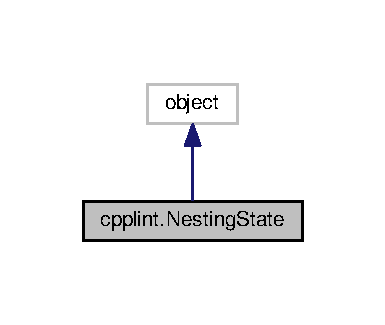
\includegraphics[width=185pt]{classcpplint_1_1NestingState__inherit__graph}
\end{center}
\end{figure}


Collaboration diagram for cpplint.\+Nesting\+State\+:\nopagebreak
\begin{figure}[H]
\begin{center}
\leavevmode
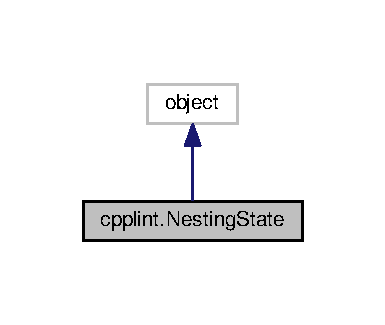
\includegraphics[width=185pt]{classcpplint_1_1NestingState__coll__graph}
\end{center}
\end{figure}
\subsection*{Public Member Functions}
\begin{DoxyCompactItemize}
\item 
def \hyperlink{classcpplint_1_1NestingState_a47e1ad559b9c7304f53d19ef6ebedab4}{\+\_\+\+\_\+init\+\_\+\+\_\+} (self)
\item 
def \hyperlink{classcpplint_1_1NestingState_a15abc0719a22ca8fbb7a8235f0e22b3e}{Seen\+Open\+Brace} (self)
\item 
def \hyperlink{classcpplint_1_1NestingState_a1a06f50d53cfe11b1f78d45b531e0c32}{In\+Namespace\+Body} (self)
\item 
def \hyperlink{classcpplint_1_1NestingState_a67aa1907d42b8408c227ff18537071c7}{In\+ExternC} (self)
\item 
def \hyperlink{classcpplint_1_1NestingState_a8e111c25149c41bd8927606244965b3c}{In\+Class\+Declaration} (self)
\item 
def \hyperlink{classcpplint_1_1NestingState_aa35a529052e4863a477eae649ce778d2}{In\+Asm\+Block} (self)
\item 
def \hyperlink{classcpplint_1_1NestingState_a8f4e9ba1aaa0459de2bedd966e7a2b54}{In\+Template\+Argument\+List} (self, clean\+\_\+lines, linenum, pos)
\item 
def \hyperlink{classcpplint_1_1NestingState_ac3d509c536af445e8ab6b17b067b53f1}{Update\+Preprocessor} (self, line)
\item 
def \hyperlink{classcpplint_1_1NestingState_a3adead8c1575b98ace5c5230f3772c1e}{Update} (self, filename, clean\+\_\+lines, linenum, error)
\item 
def \hyperlink{classcpplint_1_1NestingState_a4141768e75b16698463670caaa587120}{Innermost\+Class} (self)
\item 
def \hyperlink{classcpplint_1_1NestingState_a7bde5ab65152b4073763b1bd17cba567}{Check\+Completed\+Blocks} (self, filename, error)
\end{DoxyCompactItemize}
\subsection*{Public Attributes}
\begin{DoxyCompactItemize}
\item 
\hyperlink{classcpplint_1_1NestingState_a6ae9bea040f988d152922788d0d73a15}{stack}
\item 
\hyperlink{classcpplint_1_1NestingState_a7aa34c8fb8df73d76f702c7012c46911}{previous\+\_\+stack\+\_\+top}
\item 
\hyperlink{classcpplint_1_1NestingState_a3a5ca37e3066d91830ea1faa8feae4e5}{pp\+\_\+stack}
\end{DoxyCompactItemize}


\subsection{Detailed Description}
\begin{DoxyVerb}Holds states related to parsing braces.\end{DoxyVerb}
 

\subsection{Constructor \& Destructor Documentation}
\index{cpplint\+::\+Nesting\+State@{cpplint\+::\+Nesting\+State}!\+\_\+\+\_\+init\+\_\+\+\_\+@{\+\_\+\+\_\+init\+\_\+\+\_\+}}
\index{\+\_\+\+\_\+init\+\_\+\+\_\+@{\+\_\+\+\_\+init\+\_\+\+\_\+}!cpplint\+::\+Nesting\+State@{cpplint\+::\+Nesting\+State}}
\subsubsection[{\texorpdfstring{\+\_\+\+\_\+init\+\_\+\+\_\+(self)}{__init__(self)}}]{\setlength{\rightskip}{0pt plus 5cm}def cpplint.\+Nesting\+State.\+\_\+\+\_\+init\+\_\+\+\_\+ (
\begin{DoxyParamCaption}
\item[{}]{self}
\end{DoxyParamCaption}
)}\hypertarget{classcpplint_1_1NestingState_a47e1ad559b9c7304f53d19ef6ebedab4}{}\label{classcpplint_1_1NestingState_a47e1ad559b9c7304f53d19ef6ebedab4}


\subsection{Member Function Documentation}
\index{cpplint\+::\+Nesting\+State@{cpplint\+::\+Nesting\+State}!Check\+Completed\+Blocks@{Check\+Completed\+Blocks}}
\index{Check\+Completed\+Blocks@{Check\+Completed\+Blocks}!cpplint\+::\+Nesting\+State@{cpplint\+::\+Nesting\+State}}
\subsubsection[{\texorpdfstring{Check\+Completed\+Blocks(self, filename, error)}{CheckCompletedBlocks(self, filename, error)}}]{\setlength{\rightskip}{0pt plus 5cm}def cpplint.\+Nesting\+State.\+Check\+Completed\+Blocks (
\begin{DoxyParamCaption}
\item[{}]{self, }
\item[{}]{filename, }
\item[{}]{error}
\end{DoxyParamCaption}
)}\hypertarget{classcpplint_1_1NestingState_a7bde5ab65152b4073763b1bd17cba567}{}\label{classcpplint_1_1NestingState_a7bde5ab65152b4073763b1bd17cba567}
\begin{DoxyVerb}Checks that all classes and namespaces have been completely parsed.

Call this when all lines in a file have been processed.
Args:
  filename: The name of the current file.
  error: The function to call with any errors found.
\end{DoxyVerb}
 \index{cpplint\+::\+Nesting\+State@{cpplint\+::\+Nesting\+State}!In\+Asm\+Block@{In\+Asm\+Block}}
\index{In\+Asm\+Block@{In\+Asm\+Block}!cpplint\+::\+Nesting\+State@{cpplint\+::\+Nesting\+State}}
\subsubsection[{\texorpdfstring{In\+Asm\+Block(self)}{InAsmBlock(self)}}]{\setlength{\rightskip}{0pt plus 5cm}def cpplint.\+Nesting\+State.\+In\+Asm\+Block (
\begin{DoxyParamCaption}
\item[{}]{self}
\end{DoxyParamCaption}
)}\hypertarget{classcpplint_1_1NestingState_aa35a529052e4863a477eae649ce778d2}{}\label{classcpplint_1_1NestingState_aa35a529052e4863a477eae649ce778d2}
\begin{DoxyVerb}Check if we are currently one level inside an inline ASM block.

Returns:
  True if the top of the stack is a block containing inline ASM.
\end{DoxyVerb}
 \index{cpplint\+::\+Nesting\+State@{cpplint\+::\+Nesting\+State}!In\+Class\+Declaration@{In\+Class\+Declaration}}
\index{In\+Class\+Declaration@{In\+Class\+Declaration}!cpplint\+::\+Nesting\+State@{cpplint\+::\+Nesting\+State}}
\subsubsection[{\texorpdfstring{In\+Class\+Declaration(self)}{InClassDeclaration(self)}}]{\setlength{\rightskip}{0pt plus 5cm}def cpplint.\+Nesting\+State.\+In\+Class\+Declaration (
\begin{DoxyParamCaption}
\item[{}]{self}
\end{DoxyParamCaption}
)}\hypertarget{classcpplint_1_1NestingState_a8e111c25149c41bd8927606244965b3c}{}\label{classcpplint_1_1NestingState_a8e111c25149c41bd8927606244965b3c}
\begin{DoxyVerb}Check if we are currently one level inside a class or struct declaration.

Returns:
  True if top of the stack is a class/struct, False otherwise.
\end{DoxyVerb}
 \index{cpplint\+::\+Nesting\+State@{cpplint\+::\+Nesting\+State}!In\+ExternC@{In\+ExternC}}
\index{In\+ExternC@{In\+ExternC}!cpplint\+::\+Nesting\+State@{cpplint\+::\+Nesting\+State}}
\subsubsection[{\texorpdfstring{In\+Extern\+C(self)}{InExternC(self)}}]{\setlength{\rightskip}{0pt plus 5cm}def cpplint.\+Nesting\+State.\+In\+ExternC (
\begin{DoxyParamCaption}
\item[{}]{self}
\end{DoxyParamCaption}
)}\hypertarget{classcpplint_1_1NestingState_a67aa1907d42b8408c227ff18537071c7}{}\label{classcpplint_1_1NestingState_a67aa1907d42b8408c227ff18537071c7}
\begin{DoxyVerb}Check if we are currently one level inside an 'extern "C"' block.

Returns:
  True if top of the stack is an extern block, False otherwise.
\end{DoxyVerb}
 \index{cpplint\+::\+Nesting\+State@{cpplint\+::\+Nesting\+State}!In\+Namespace\+Body@{In\+Namespace\+Body}}
\index{In\+Namespace\+Body@{In\+Namespace\+Body}!cpplint\+::\+Nesting\+State@{cpplint\+::\+Nesting\+State}}
\subsubsection[{\texorpdfstring{In\+Namespace\+Body(self)}{InNamespaceBody(self)}}]{\setlength{\rightskip}{0pt plus 5cm}def cpplint.\+Nesting\+State.\+In\+Namespace\+Body (
\begin{DoxyParamCaption}
\item[{}]{self}
\end{DoxyParamCaption}
)}\hypertarget{classcpplint_1_1NestingState_a1a06f50d53cfe11b1f78d45b531e0c32}{}\label{classcpplint_1_1NestingState_a1a06f50d53cfe11b1f78d45b531e0c32}
\begin{DoxyVerb}Check if we are currently one level inside a namespace body.

Returns:
  True if top of the stack is a namespace block, False otherwise.
\end{DoxyVerb}
 \index{cpplint\+::\+Nesting\+State@{cpplint\+::\+Nesting\+State}!Innermost\+Class@{Innermost\+Class}}
\index{Innermost\+Class@{Innermost\+Class}!cpplint\+::\+Nesting\+State@{cpplint\+::\+Nesting\+State}}
\subsubsection[{\texorpdfstring{Innermost\+Class(self)}{InnermostClass(self)}}]{\setlength{\rightskip}{0pt plus 5cm}def cpplint.\+Nesting\+State.\+Innermost\+Class (
\begin{DoxyParamCaption}
\item[{}]{self}
\end{DoxyParamCaption}
)}\hypertarget{classcpplint_1_1NestingState_a4141768e75b16698463670caaa587120}{}\label{classcpplint_1_1NestingState_a4141768e75b16698463670caaa587120}
\begin{DoxyVerb}Get class info on the top of the stack.

Returns:
  A _ClassInfo object if we are inside a class, or None otherwise.
\end{DoxyVerb}
 \index{cpplint\+::\+Nesting\+State@{cpplint\+::\+Nesting\+State}!In\+Template\+Argument\+List@{In\+Template\+Argument\+List}}
\index{In\+Template\+Argument\+List@{In\+Template\+Argument\+List}!cpplint\+::\+Nesting\+State@{cpplint\+::\+Nesting\+State}}
\subsubsection[{\texorpdfstring{In\+Template\+Argument\+List(self, clean\+\_\+lines, linenum, pos)}{InTemplateArgumentList(self, clean_lines, linenum, pos)}}]{\setlength{\rightskip}{0pt plus 5cm}def cpplint.\+Nesting\+State.\+In\+Template\+Argument\+List (
\begin{DoxyParamCaption}
\item[{}]{self, }
\item[{}]{clean\+\_\+lines, }
\item[{}]{linenum, }
\item[{}]{pos}
\end{DoxyParamCaption}
)}\hypertarget{classcpplint_1_1NestingState_a8f4e9ba1aaa0459de2bedd966e7a2b54}{}\label{classcpplint_1_1NestingState_a8f4e9ba1aaa0459de2bedd966e7a2b54}
\begin{DoxyVerb}Check if current position is inside template argument list.

Args:
  clean_lines: A CleansedLines instance containing the file.
  linenum: The number of the line to check.
  pos: position just after the suspected template argument.
Returns:
  True if (linenum, pos) is inside template arguments.
\end{DoxyVerb}
 \index{cpplint\+::\+Nesting\+State@{cpplint\+::\+Nesting\+State}!Seen\+Open\+Brace@{Seen\+Open\+Brace}}
\index{Seen\+Open\+Brace@{Seen\+Open\+Brace}!cpplint\+::\+Nesting\+State@{cpplint\+::\+Nesting\+State}}
\subsubsection[{\texorpdfstring{Seen\+Open\+Brace(self)}{SeenOpenBrace(self)}}]{\setlength{\rightskip}{0pt plus 5cm}def cpplint.\+Nesting\+State.\+Seen\+Open\+Brace (
\begin{DoxyParamCaption}
\item[{}]{self}
\end{DoxyParamCaption}
)}\hypertarget{classcpplint_1_1NestingState_a15abc0719a22ca8fbb7a8235f0e22b3e}{}\label{classcpplint_1_1NestingState_a15abc0719a22ca8fbb7a8235f0e22b3e}
\begin{DoxyVerb}Check if we have seen the opening brace for the innermost block.

Returns:
  True if we have seen the opening brace, False if the innermost
  block is still expecting an opening brace.
\end{DoxyVerb}
 \index{cpplint\+::\+Nesting\+State@{cpplint\+::\+Nesting\+State}!Update@{Update}}
\index{Update@{Update}!cpplint\+::\+Nesting\+State@{cpplint\+::\+Nesting\+State}}
\subsubsection[{\texorpdfstring{Update(self, filename, clean\+\_\+lines, linenum, error)}{Update(self, filename, clean_lines, linenum, error)}}]{\setlength{\rightskip}{0pt plus 5cm}def cpplint.\+Nesting\+State.\+Update (
\begin{DoxyParamCaption}
\item[{}]{self, }
\item[{}]{filename, }
\item[{}]{clean\+\_\+lines, }
\item[{}]{linenum, }
\item[{}]{error}
\end{DoxyParamCaption}
)}\hypertarget{classcpplint_1_1NestingState_a3adead8c1575b98ace5c5230f3772c1e}{}\label{classcpplint_1_1NestingState_a3adead8c1575b98ace5c5230f3772c1e}
\begin{DoxyVerb}Update nesting state with current line.

Args:
  filename: The name of the current file.
  clean_lines: A CleansedLines instance containing the file.
  linenum: The number of the line to check.
  error: The function to call with any errors found.
\end{DoxyVerb}
 \index{cpplint\+::\+Nesting\+State@{cpplint\+::\+Nesting\+State}!Update\+Preprocessor@{Update\+Preprocessor}}
\index{Update\+Preprocessor@{Update\+Preprocessor}!cpplint\+::\+Nesting\+State@{cpplint\+::\+Nesting\+State}}
\subsubsection[{\texorpdfstring{Update\+Preprocessor(self, line)}{UpdatePreprocessor(self, line)}}]{\setlength{\rightskip}{0pt plus 5cm}def cpplint.\+Nesting\+State.\+Update\+Preprocessor (
\begin{DoxyParamCaption}
\item[{}]{self, }
\item[{}]{line}
\end{DoxyParamCaption}
)}\hypertarget{classcpplint_1_1NestingState_ac3d509c536af445e8ab6b17b067b53f1}{}\label{classcpplint_1_1NestingState_ac3d509c536af445e8ab6b17b067b53f1}
\begin{DoxyVerb}Update preprocessor stack.

We need to handle preprocessors due to classes like this:
  #ifdef SWIG
  struct ResultDetailsPageElementExtensionPoint {
  #else
  struct ResultDetailsPageElementExtensionPoint : public Extension {
  #endif

We make the following assumptions (good enough for most files):
- Preprocessor condition evaluates to true from #if up to first
  #else/#elif/#endif.

- Preprocessor condition evaluates to false from #else/#elif up
  to #endif.  We still perform lint checks on these lines, but
  these do not affect nesting stack.

Args:
  line: current line to check.
\end{DoxyVerb}
 

\subsection{Member Data Documentation}
\index{cpplint\+::\+Nesting\+State@{cpplint\+::\+Nesting\+State}!pp\+\_\+stack@{pp\+\_\+stack}}
\index{pp\+\_\+stack@{pp\+\_\+stack}!cpplint\+::\+Nesting\+State@{cpplint\+::\+Nesting\+State}}
\subsubsection[{\texorpdfstring{pp\+\_\+stack}{pp_stack}}]{\setlength{\rightskip}{0pt plus 5cm}cpplint.\+Nesting\+State.\+pp\+\_\+stack}\hypertarget{classcpplint_1_1NestingState_a3a5ca37e3066d91830ea1faa8feae4e5}{}\label{classcpplint_1_1NestingState_a3a5ca37e3066d91830ea1faa8feae4e5}
\index{cpplint\+::\+Nesting\+State@{cpplint\+::\+Nesting\+State}!previous\+\_\+stack\+\_\+top@{previous\+\_\+stack\+\_\+top}}
\index{previous\+\_\+stack\+\_\+top@{previous\+\_\+stack\+\_\+top}!cpplint\+::\+Nesting\+State@{cpplint\+::\+Nesting\+State}}
\subsubsection[{\texorpdfstring{previous\+\_\+stack\+\_\+top}{previous_stack_top}}]{\setlength{\rightskip}{0pt plus 5cm}cpplint.\+Nesting\+State.\+previous\+\_\+stack\+\_\+top}\hypertarget{classcpplint_1_1NestingState_a7aa34c8fb8df73d76f702c7012c46911}{}\label{classcpplint_1_1NestingState_a7aa34c8fb8df73d76f702c7012c46911}
\index{cpplint\+::\+Nesting\+State@{cpplint\+::\+Nesting\+State}!stack@{stack}}
\index{stack@{stack}!cpplint\+::\+Nesting\+State@{cpplint\+::\+Nesting\+State}}
\subsubsection[{\texorpdfstring{stack}{stack}}]{\setlength{\rightskip}{0pt plus 5cm}cpplint.\+Nesting\+State.\+stack}\hypertarget{classcpplint_1_1NestingState_a6ae9bea040f988d152922788d0d73a15}{}\label{classcpplint_1_1NestingState_a6ae9bea040f988d152922788d0d73a15}


The documentation for this class was generated from the following file\+:\begin{DoxyCompactItemize}
\item 
\hyperlink{cpplint_8py}{cpplint.\+py}\end{DoxyCompactItemize}

\hypertarget{classpassCustStr}{}\section{pass\+Cust\+Str Class Reference}
\label{classpassCustStr}\index{pass\+Cust\+Str@{pass\+Cust\+Str}}


{\ttfamily \#include $<$pass\+Cust\+Str.\+hpp$>$}

\subsection*{Public Member Functions}
\begin{DoxyCompactItemize}
\item 
bool \hyperlink{classpassCustStr_a997766f5e24240b515062346f2f0dd18}{change} (beginner\+\_\+tutorials\+::\+Change\+String\+::\+Request \&req, beginner\+\_\+tutorials\+::\+Change\+String\+::\+Response \&res)
\end{DoxyCompactItemize}
\subsection*{Public Attributes}
\begin{DoxyCompactItemize}
\item 
std\+::string \hyperlink{classpassCustStr_a3ce7263adc4bbc1d6b621c35a9da4f62}{request\+Data}
\end{DoxyCompactItemize}


\subsection{Member Function Documentation}
\index{pass\+Cust\+Str@{pass\+Cust\+Str}!change@{change}}
\index{change@{change}!pass\+Cust\+Str@{pass\+Cust\+Str}}
\subsubsection[{\texorpdfstring{change(beginner\+\_\+tutorials\+::\+Change\+String\+::\+Request \&req, beginner\+\_\+tutorials\+::\+Change\+String\+::\+Response \&res)}{change(beginner_tutorials::ChangeString::Request &req, beginner_tutorials::ChangeString::Response &res)}}]{\setlength{\rightskip}{0pt plus 5cm}bool pass\+Cust\+Str\+::change (
\begin{DoxyParamCaption}
\item[{beginner\+\_\+tutorials\+::\+Change\+String\+::\+Request \&}]{req, }
\item[{beginner\+\_\+tutorials\+::\+Change\+String\+::\+Response \&}]{res}
\end{DoxyParamCaption}
)}\hypertarget{classpassCustStr_a997766f5e24240b515062346f2f0dd18}{}\label{classpassCustStr_a997766f5e24240b515062346f2f0dd18}
This member function is used as a callback for the change\+\_\+string service. This is needed because global string is strictly prohibited.

This member function is a bool type, it takes the arguments from the change\+\_\+string service. 
\begin{DoxyParams}{Parameters}
{\em beginner\+\_\+tutorials\+::\+Change\+String\+::\+Request} & \\
\hline
{\em beginner\+\_\+tutorials\+::\+Change\+String\+::\+Response} & \\
\hline
\end{DoxyParams}


\subsection{Member Data Documentation}
\index{pass\+Cust\+Str@{pass\+Cust\+Str}!request\+Data@{request\+Data}}
\index{request\+Data@{request\+Data}!pass\+Cust\+Str@{pass\+Cust\+Str}}
\subsubsection[{\texorpdfstring{request\+Data}{requestData}}]{\setlength{\rightskip}{0pt plus 5cm}std\+::string pass\+Cust\+Str\+::request\+Data}\hypertarget{classpassCustStr_a3ce7263adc4bbc1d6b621c35a9da4f62}{}\label{classpassCustStr_a3ce7263adc4bbc1d6b621c35a9da4f62}
$<$ This global string variable accepts a user-\/defined string from the change\+\_\+string service. 

The documentation for this class was generated from the following files\+:\begin{DoxyCompactItemize}
\item 
include/\hyperlink{passCustStr_8hpp}{pass\+Cust\+Str.\+hpp}\item 
src/\hyperlink{passCustStr_8cpp}{pass\+Cust\+Str.\+cpp}\end{DoxyCompactItemize}

\chapter{File Documentation}
\hypertarget{CMakeLists_8txt}{}\section{C\+Make\+Lists.\+txt File Reference}
\label{CMakeLists_8txt}\index{C\+Make\+Lists.\+txt@{C\+Make\+Lists.\+txt}}
\subsection*{Functions}
\begin{DoxyCompactItemize}
\item 
\hyperlink{CMakeLists_8txt_a257873ea53487c7f7f72678d9fcbbd0d}{cmake\+\_\+minimum\+\_\+required} (V\+E\+R\+S\+I\+ON 2.\+8.\+3) project(beginner\+\_\+tutorials) find\+\_\+package(catkin R\+E\+Q\+U\+I\+R\+ED C\+O\+M\+P\+O\+N\+E\+N\+TS roscpp rospy std\+\_\+msgs genmsg message\+\_\+generation) add\+\_\+service\+\_\+files(F\+I\+L\+ES Add\+Two\+Ints.\+srv Change\+String.\+srv) generate\+\_\+messages(D\+E\+P\+E\+N\+D\+E\+N\+C\+I\+ES std\+\_\+msgs) catkin\+\_\+package() include\+\_\+directories(include \$
\item 
\hyperlink{CMakeLists_8txt_a40715d33c1a048014457a014e14ff703}{add\+\_\+executable} (talker src/talker.\+cpp) target\+\_\+link\+\_\+libraries(talker \$
\item 
\hyperlink{CMakeLists_8txt_a1f028819c1eefa47f1f413c6954f0ddb}{add\+\_\+dependencies} (talker beginner\+\_\+tutorials\+\_\+generate\+\_\+messages\+\_\+cpp beginner\+\_\+tutorials\+\_\+gencpp) \hyperlink{CMakeLists_8txt_a40715d33c1a048014457a014e14ff703}{add\+\_\+executable}(listener src/listener.\+cpp) target\+\_\+link\+\_\+libraries(listener \$
\item 
\hyperlink{CMakeLists_8txt_aff6b4efc61b9086ee7e78ad0c8eb5b05}{add\+\_\+dependencies} (listener beginner\+\_\+tutorials\+\_\+generate\+\_\+messages\+\_\+cpp) \hyperlink{CMakeLists_8txt_a40715d33c1a048014457a014e14ff703}{add\+\_\+executable}(change\+\_\+string\+\_\+client src/change\+\_\+string\+\_\+client.\+cpp) target\+\_\+link\+\_\+libraries(change\+\_\+string\+\_\+client \$
\end{DoxyCompactItemize}


\subsection{Function Documentation}
\index{C\+Make\+Lists.\+txt@{C\+Make\+Lists.\+txt}!add\+\_\+dependencies@{add\+\_\+dependencies}}
\index{add\+\_\+dependencies@{add\+\_\+dependencies}!C\+Make\+Lists.\+txt@{C\+Make\+Lists.\+txt}}
\subsubsection[{\texorpdfstring{add\+\_\+dependencies(talker beginner\+\_\+tutorials\+\_\+generate\+\_\+messages\+\_\+cpp beginner\+\_\+tutorials\+\_\+gencpp) add\+\_\+executable(listener src/listener.\+cpp) target\+\_\+link\+\_\+libraries(listener \$}{add_dependencies(talker beginner_tutorials_generate_messages_cpp beginner_tutorials_gencpp) add_executable(listener src/listener.cpp) target_link_libraries(listener $}}]{\setlength{\rightskip}{0pt plus 5cm}add\+\_\+dependencies (
\begin{DoxyParamCaption}
\item[{talker beginner\+\_\+tutorials\+\_\+generate\+\_\+messages\+\_\+cpp}]{beginner\+\_\+tutorials\+\_\+gencpp}
\end{DoxyParamCaption}
)}\hypertarget{CMakeLists_8txt_a1f028819c1eefa47f1f413c6954f0ddb}{}\label{CMakeLists_8txt_a1f028819c1eefa47f1f413c6954f0ddb}
\index{C\+Make\+Lists.\+txt@{C\+Make\+Lists.\+txt}!add\+\_\+dependencies@{add\+\_\+dependencies}}
\index{add\+\_\+dependencies@{add\+\_\+dependencies}!C\+Make\+Lists.\+txt@{C\+Make\+Lists.\+txt}}
\subsubsection[{\texorpdfstring{add\+\_\+dependencies(listener beginner\+\_\+tutorials\+\_\+generate\+\_\+messages\+\_\+cpp) add\+\_\+executable(change\+\_\+string\+\_\+client src/change\+\_\+string\+\_\+client.\+cpp) target\+\_\+link\+\_\+libraries(change\+\_\+string\+\_\+client \$}{add_dependencies(listener beginner_tutorials_generate_messages_cpp) add_executable(change_string_client src/change_string_client.cpp) target_link_libraries(change_string_client $}}]{\setlength{\rightskip}{0pt plus 5cm}add\+\_\+dependencies (
\begin{DoxyParamCaption}
\item[{listener beginner\+\_\+tutorials\+\_\+generate\+\_\+messages\+\_\+cpp}]{}
\end{DoxyParamCaption}
)}\hypertarget{CMakeLists_8txt_aff6b4efc61b9086ee7e78ad0c8eb5b05}{}\label{CMakeLists_8txt_aff6b4efc61b9086ee7e78ad0c8eb5b05}
\index{C\+Make\+Lists.\+txt@{C\+Make\+Lists.\+txt}!add\+\_\+executable@{add\+\_\+executable}}
\index{add\+\_\+executable@{add\+\_\+executable}!C\+Make\+Lists.\+txt@{C\+Make\+Lists.\+txt}}
\subsubsection[{\texorpdfstring{add\+\_\+executable(talker src/talker.\+cpp) target\+\_\+link\+\_\+libraries(talker \$}{add_executable(talker src/talker.cpp) target_link_libraries(talker $}}]{\setlength{\rightskip}{0pt plus 5cm}add\+\_\+executable (
\begin{DoxyParamCaption}
\item[{talker src/talker.}]{cpp}
\end{DoxyParamCaption}
)}\hypertarget{CMakeLists_8txt_a40715d33c1a048014457a014e14ff703}{}\label{CMakeLists_8txt_a40715d33c1a048014457a014e14ff703}
\index{C\+Make\+Lists.\+txt@{C\+Make\+Lists.\+txt}!cmake\+\_\+minimum\+\_\+required@{cmake\+\_\+minimum\+\_\+required}}
\index{cmake\+\_\+minimum\+\_\+required@{cmake\+\_\+minimum\+\_\+required}!C\+Make\+Lists.\+txt@{C\+Make\+Lists.\+txt}}
\subsubsection[{\texorpdfstring{cmake\+\_\+minimum\+\_\+required(\+V\+E\+R\+S\+I\+O\+N 2.\+8.\+3) project(beginner\+\_\+tutorials) find\+\_\+package(catkin R\+E\+Q\+U\+I\+R\+E\+D C\+O\+M\+P\+O\+N\+E\+N\+T\+S roscpp rospy std\+\_\+msgs genmsg message\+\_\+generation) add\+\_\+service\+\_\+files(\+F\+I\+L\+E\+S Add\+Two\+Ints.\+srv Change\+String.\+srv) generate\+\_\+messages(\+D\+E\+P\+E\+N\+D\+E\+N\+C\+I\+E\+S std\+\_\+msgs) catkin\+\_\+package() include\+\_\+directories(include \$}{cmake_minimum_required(VERSION 2.8.3) project(beginner_tutorials) find_package(catkin REQUIRED COMPONENTS roscpp rospy std_msgs genmsg message_generation) add_service_files(FILES AddTwoInts.srv ChangeString.srv) generate_messages(DEPENDENCIES std_msgs) catkin_package() include_directories(include $}}]{\setlength{\rightskip}{0pt plus 5cm}cmake\+\_\+minimum\+\_\+required (
\begin{DoxyParamCaption}
\item[{V\+E\+R\+S\+I\+ON 2.\+8.}]{3}
\end{DoxyParamCaption}
)}\hypertarget{CMakeLists_8txt_a257873ea53487c7f7f72678d9fcbbd0d}{}\label{CMakeLists_8txt_a257873ea53487c7f7f72678d9fcbbd0d}

\hypertarget{cppcheck_8txt}{}\section{cppcheck.\+txt File Reference}
\label{cppcheck_8txt}\index{cppcheck.\+txt@{cppcheck.\+txt}}

\hypertarget{cpplint_8py}{}\section{cpplint.\+py File Reference}
\label{cpplint_8py}\index{cpplint.\+py@{cpplint.\+py}}
\subsection*{Classes}
\begin{DoxyCompactItemize}
\item 
class \hyperlink{classcpplint_1_1__IncludeState}{cpplint.\+\_\+\+Include\+State}
\item 
class \hyperlink{classcpplint_1_1__CppLintState}{cpplint.\+\_\+\+Cpp\+Lint\+State}
\item 
class \hyperlink{classcpplint_1_1__FunctionState}{cpplint.\+\_\+\+Function\+State}
\item 
class \hyperlink{classcpplint_1_1__IncludeError}{cpplint.\+\_\+\+Include\+Error}
\item 
class \hyperlink{classcpplint_1_1FileInfo}{cpplint.\+File\+Info}
\item 
class \hyperlink{classcpplint_1_1CleansedLines}{cpplint.\+Cleansed\+Lines}
\item 
class \hyperlink{classcpplint_1_1__BlockInfo}{cpplint.\+\_\+\+Block\+Info}
\item 
class \hyperlink{classcpplint_1_1__ExternCInfo}{cpplint.\+\_\+\+Extern\+C\+Info}
\item 
class \hyperlink{classcpplint_1_1__ClassInfo}{cpplint.\+\_\+\+Class\+Info}
\item 
class \hyperlink{classcpplint_1_1__NamespaceInfo}{cpplint.\+\_\+\+Namespace\+Info}
\item 
class \hyperlink{classcpplint_1_1__PreprocessorInfo}{cpplint.\+\_\+\+Preprocessor\+Info}
\item 
class \hyperlink{classcpplint_1_1NestingState}{cpplint.\+Nesting\+State}
\end{DoxyCompactItemize}
\subsection*{Namespaces}
\begin{DoxyCompactItemize}
\item 
 \hyperlink{namespacecpplint}{cpplint}
\end{DoxyCompactItemize}
\subsection*{Functions}
\begin{DoxyCompactItemize}
\item 
def \hyperlink{namespacecpplint_a28e546a8f20e32ef7dcf4ecbecd8b367}{cpplint.\+Process\+Hpp\+Headers\+Option} (val)
\item 
def \hyperlink{namespacecpplint_ad4fd5ecbae967884b0a77ee8b3ba1e16}{cpplint.\+Is\+Header\+Extension} (file\+\_\+extension)
\item 
def \hyperlink{namespacecpplint_a52ae8f1d9436d14ddb94ceed06026c43}{cpplint.\+Parse\+Nolint\+Suppressions} (filename, raw\+\_\+line, linenum, error)
\item 
def \hyperlink{namespacecpplint_a316dc237dc0cde7bafec3c30d5624cac}{cpplint.\+Process\+Global\+Suppresions} (lines)
\item 
def \hyperlink{namespacecpplint_a1d92dc3582da477f98ab5b85bd13fea0}{cpplint.\+Reset\+Nolint\+Suppressions} ()
\item 
def \hyperlink{namespacecpplint_a0b9e1f991f1a3d02cda3234784241d1f}{cpplint.\+Is\+Error\+Suppressed\+By\+Nolint} (category, linenum)
\item 
def \hyperlink{namespacecpplint_a73ac2ecfcd9c52b4a3755176c68dea7e}{cpplint.\+Match} (pattern, s)
\item 
def \hyperlink{namespacecpplint_a1b85a5657aeab8b4a0ed85e06aed3576}{cpplint.\+Replace\+All} (pattern, rep, s)
\item 
def \hyperlink{namespacecpplint_a75eae6bb88590e904f751502c8ee4bab}{cpplint.\+Search} (pattern, s)
\item 
def \hyperlink{namespacecpplint_ae51e76d6d73b36b9e965d2ac9d21d7c2}{cpplint.\+Error} (filename, linenum, category, confidence, message)
\item 
def \hyperlink{namespacecpplint_a034b93866a853c2e21577fb371a7fa9d}{cpplint.\+Is\+Cpp\+String} (line)
\item 
def \hyperlink{namespacecpplint_a61b3f81ef467e7cb417d13e9051180fc}{cpplint.\+Cleanse\+Raw\+Strings} (raw\+\_\+lines)
\item 
def \hyperlink{namespacecpplint_af0404401670283c9d4f948180e427401}{cpplint.\+Find\+Next\+Multi\+Line\+Comment\+Start} (lines, lineix)
\item 
def \hyperlink{namespacecpplint_a4965d6f615333f43155d9e430471e228}{cpplint.\+Find\+Next\+Multi\+Line\+Comment\+End} (lines, lineix)
\item 
def \hyperlink{namespacecpplint_a3a5f71cdc2e78491b4bedde8a0103679}{cpplint.\+Remove\+Multi\+Line\+Comments\+From\+Range} (lines, begin, end)
\item 
def \hyperlink{namespacecpplint_ac259a6d0f292aeec05dee7ca312e1fc2}{cpplint.\+Remove\+Multi\+Line\+Comments} (filename, lines, error)
\item 
def \hyperlink{namespacecpplint_ad795aa89f263838ec59fb0e7c52c842a}{cpplint.\+Cleanse\+Comments} (line)
\item 
def \hyperlink{namespacecpplint_a6e623c46c1ae3bf650454744a693a633}{cpplint.\+Find\+End\+Of\+Expression\+In\+Line} (line, startpos, stack)
\item 
def \hyperlink{namespacecpplint_af254258f584f59c87fcfd755e3c9017a}{cpplint.\+Close\+Expression} (clean\+\_\+lines, linenum, pos)
\item 
def \hyperlink{namespacecpplint_a8572f47efb3bc11632d1192fd74bb7eb}{cpplint.\+Find\+Start\+Of\+Expression\+In\+Line} (line, endpos, stack)
\item 
def \hyperlink{namespacecpplint_a15cd96cbf1c13e655e156fbd98cf0bae}{cpplint.\+Reverse\+Close\+Expression} (clean\+\_\+lines, linenum, pos)
\item 
def \hyperlink{namespacecpplint_a0ad6bf921300c829db3696b81fa52d20}{cpplint.\+Check\+For\+Copyright} (filename, lines, error)
\item 
def \hyperlink{namespacecpplint_a1b5cb7c1367845d7c7079eac5ea61dc8}{cpplint.\+Get\+Indent\+Level} (line)
\item 
def \hyperlink{namespacecpplint_a3f143d4e8f70c0fd05e3f0ce81b0cc9a}{cpplint.\+Get\+Header\+Guard\+C\+P\+P\+Variable} (filename)
\item 
def \hyperlink{namespacecpplint_a3694fa1b195f49a0d78dfc81ee665eec}{cpplint.\+Check\+For\+Header\+Guard} (filename, clean\+\_\+lines, error)
\item 
def \hyperlink{namespacecpplint_ab549dcced7ca1d4b24538ec52b42439e}{cpplint.\+Check\+Header\+File\+Included} (filename, include\+\_\+state, error)
\item 
def \hyperlink{namespacecpplint_a03c0e0d285b02b0e26ec514761654da8}{cpplint.\+Check\+For\+Bad\+Characters} (filename, lines, error)
\item 
def \hyperlink{namespacecpplint_a7a594af230939932174dd5743088027d}{cpplint.\+Check\+For\+Newline\+At\+E\+OF} (filename, lines, error)
\item 
def \hyperlink{namespacecpplint_a81c4baf76bde576f56661c22d01e470d}{cpplint.\+Check\+For\+Multiline\+Comments\+And\+Strings} (filename, clean\+\_\+lines, linenum, error)
\item 
def \hyperlink{namespacecpplint_a9c406c00843a2c47058b1e9dec4e5b11}{cpplint.\+Check\+Posix\+Threading} (filename, clean\+\_\+lines, linenum, error)
\item 
def \hyperlink{namespacecpplint_ab066834feaa7bf5a92982bbfb0af89c1}{cpplint.\+Check\+Vlog\+Arguments} (filename, clean\+\_\+lines, linenum, error)
\item 
def \hyperlink{namespacecpplint_a8b47da46bc61f72ab12e9228acc3a0cd}{cpplint.\+Check\+Invalid\+Increment} (filename, clean\+\_\+lines, linenum, error)
\item 
def \hyperlink{namespacecpplint_a5a95ee1e23638e172a3361723503329c}{cpplint.\+Is\+Macro\+Definition} (clean\+\_\+lines, linenum)
\item 
def \hyperlink{namespacecpplint_adde7d60b6354b40d9ef9acda6e847d7b}{cpplint.\+Is\+Forward\+Class\+Declaration} (clean\+\_\+lines, linenum)
\item 
def \hyperlink{namespacecpplint_a954b179c4037e5da8ac599cce095c37e}{cpplint.\+Check\+For\+Non\+Standard\+Constructs} (filename, clean\+\_\+lines, linenum, nesting\+\_\+state, error)
\item 
def \hyperlink{namespacecpplint_a2ea8b2c917d5ce466287e1c6fe26f0db}{cpplint.\+Check\+Spacing\+For\+Function\+Call} (filename, clean\+\_\+lines, linenum, error)
\item 
def \hyperlink{namespacecpplint_adf59429f3dd145e978624fe239809260}{cpplint.\+Is\+Blank\+Line} (line)
\item 
def \hyperlink{namespacecpplint_a7c5964127d06521a2a05fbb28cc26478}{cpplint.\+Check\+For\+Namespace\+Indentation} (filename, nesting\+\_\+state, clean\+\_\+lines, line, error)
\item 
def \hyperlink{namespacecpplint_a2699a7cad55a82cab5f73c012747203e}{cpplint.\+Check\+For\+Function\+Lengths} (filename, clean\+\_\+lines, linenum, function\+\_\+state, error)
\item 
def \hyperlink{namespacecpplint_af126b85f4c25f359c40ce349f4eb7a2d}{cpplint.\+Check\+Comment} (line, filename, linenum, next\+\_\+line\+\_\+start, error)
\item 
def \hyperlink{namespacecpplint_a73e82f51a8d59c816db26b5f797b3431}{cpplint.\+Check\+Spacing} (filename, clean\+\_\+lines, linenum, nesting\+\_\+state, error)
\item 
def \hyperlink{namespacecpplint_a6a15b27f48cfd70fbf76f595c34f6d9e}{cpplint.\+Check\+Operator\+Spacing} (filename, clean\+\_\+lines, linenum, error)
\item 
def \hyperlink{namespacecpplint_aacf5fa793ab27c7038e376d6a4c53d87}{cpplint.\+Check\+Parenthesis\+Spacing} (filename, clean\+\_\+lines, linenum, error)
\item 
def \hyperlink{namespacecpplint_a46d2c48a2d4e747feee44616af987bdf}{cpplint.\+Check\+Comma\+Spacing} (filename, clean\+\_\+lines, linenum, error)
\item 
def \hyperlink{namespacecpplint_a205bb76a59359eb1c0be86567bbc5256}{cpplint.\+Check\+Braces\+Spacing} (filename, clean\+\_\+lines, linenum, nesting\+\_\+state, error)
\item 
def \hyperlink{namespacecpplint_a6e55ab13af2fa8b8e1f50e09aed592b8}{cpplint.\+Is\+Decltype} (clean\+\_\+lines, linenum, column)
\item 
def \hyperlink{namespacecpplint_abc4e2f3f48debd6ae3a9561d052a955b}{cpplint.\+Check\+Section\+Spacing} (filename, clean\+\_\+lines, class\+\_\+info, linenum, error)
\item 
def \hyperlink{namespacecpplint_a27743480b080a71eb8a0320da2ca0fa3}{cpplint.\+Get\+Previous\+Non\+Blank\+Line} (clean\+\_\+lines, linenum)
\item 
def \hyperlink{namespacecpplint_a3f0a4d2ab1846bf487c742dc88946e3e}{cpplint.\+Check\+Braces} (filename, clean\+\_\+lines, linenum, error)
\item 
def \hyperlink{namespacecpplint_a725663cb5a341fbf726f2ac8fa4e61a3}{cpplint.\+Check\+Trailing\+Semicolon} (filename, clean\+\_\+lines, linenum, error)
\item 
def \hyperlink{namespacecpplint_a9c8aa68644d8cb55497a7d9cb8fb12d1}{cpplint.\+Check\+Empty\+Block\+Body} (filename, clean\+\_\+lines, linenum, error)
\item 
def \hyperlink{namespacecpplint_aefff9c2eefe99656a226d11ce4d9b555}{cpplint.\+Find\+Check\+Macro} (line)
\item 
def \hyperlink{namespacecpplint_afc5b544f640cd11be2665e6bb4646de7}{cpplint.\+Check\+Check} (filename, clean\+\_\+lines, linenum, error)
\item 
def \hyperlink{namespacecpplint_a47f66a697e177c06b56491613fbc2d38}{cpplint.\+Check\+Alt\+Tokens} (filename, clean\+\_\+lines, linenum, error)
\item 
def \hyperlink{namespacecpplint_ae55f74f34d41b59cf262511c5944209a}{cpplint.\+Get\+Line\+Width} (line)
\item 
def \hyperlink{namespacecpplint_acfc546daa5947842cb01af319dcb482b}{cpplint.\+Check\+Style} (filename, clean\+\_\+lines, linenum, file\+\_\+extension, nesting\+\_\+state, error)
\item 
def \hyperlink{namespacecpplint_add7eb8486a182205bb86de635db01384}{cpplint.\+Check\+Include\+Line} (filename, clean\+\_\+lines, linenum, include\+\_\+state, error)
\item 
def \hyperlink{namespacecpplint_a6992d951cf4be06500f6b392ee6a8111}{cpplint.\+Check\+Language} (filename, clean\+\_\+lines, linenum, file\+\_\+extension, include\+\_\+state, nesting\+\_\+state, error)
\item 
def \hyperlink{namespacecpplint_a64fc322bcf08988b43f003ff495fbabb}{cpplint.\+Check\+Global\+Static} (filename, clean\+\_\+lines, linenum, error)
\item 
def \hyperlink{namespacecpplint_aaa8b988b9e83ad1c8964ecc0739d52e5}{cpplint.\+Check\+Printf} (filename, clean\+\_\+lines, linenum, error)
\item 
def \hyperlink{namespacecpplint_ac8519cf084d818c931eac29994b03f55}{cpplint.\+Is\+Derived\+Function} (clean\+\_\+lines, linenum)
\item 
def \hyperlink{namespacecpplint_a52e4468f674e140c256254eb0d1cf007}{cpplint.\+Is\+Out\+Of\+Line\+Method\+Definition} (clean\+\_\+lines, linenum)
\item 
def \hyperlink{namespacecpplint_ae06fb1dd669681214573c0441b7e854f}{cpplint.\+Is\+Initializer\+List} (clean\+\_\+lines, linenum)
\item 
def \hyperlink{namespacecpplint_a97f01c7d6e7e6d38b52744ab393d4160}{cpplint.\+Check\+For\+Non\+Const\+Reference} (filename, clean\+\_\+lines, linenum, nesting\+\_\+state, error)
\item 
def \hyperlink{namespacecpplint_a59c5f44ae1dbedad109809d46e80588e}{cpplint.\+Check\+Casts} (filename, clean\+\_\+lines, linenum, error)
\item 
def \hyperlink{namespacecpplint_ac23d9b29d869054db2ece1e7d5196349}{cpplint.\+Check\+C\+Style\+Cast} (filename, clean\+\_\+lines, linenum, cast\+\_\+type, pattern, error)
\item 
def \hyperlink{namespacecpplint_a7657def0315cfe229ba436632f2d5042}{cpplint.\+Expecting\+Function\+Args} (clean\+\_\+lines, linenum)
\item 
def \hyperlink{namespacecpplint_a66083e7d453e845a2751e76043fcd9ea}{cpplint.\+Files\+Belong\+To\+Same\+Module} (filename\+\_\+cc, filename\+\_\+h)
\item 
def \hyperlink{namespacecpplint_a127416bee5c376937479b3119a727817}{cpplint.\+Update\+Include\+State} (filename, include\+\_\+dict, io=codecs)
\item 
def \hyperlink{namespacecpplint_a8e1a5bea9f77246f8a0ae98a23d8d04e}{cpplint.\+Check\+For\+Include\+What\+You\+Use} (filename, clean\+\_\+lines, include\+\_\+state, error, io=codecs)
\item 
def \hyperlink{namespacecpplint_add392d0ab0e8bcfeea6d02410229a0cc}{cpplint.\+Check\+Make\+Pair\+Uses\+Deduction} (filename, clean\+\_\+lines, linenum, error)
\item 
def \hyperlink{namespacecpplint_a828985bee0575cfbb64212db74b61d9a}{cpplint.\+Check\+Redundant\+Virtual} (filename, clean\+\_\+lines, linenum, error)
\item 
def \hyperlink{namespacecpplint_ab4f9b0390c702f149cec4030901d249d}{cpplint.\+Check\+Redundant\+Override\+Or\+Final} (filename, clean\+\_\+lines, linenum, error)
\item 
def \hyperlink{namespacecpplint_a618e046738f246f01972bce339ee5d49}{cpplint.\+Is\+Block\+In\+Name\+Space} (nesting\+\_\+state, is\+\_\+forward\+\_\+declaration)
\item 
def \hyperlink{namespacecpplint_aaaeb792789007d86b0898676c00caa72}{cpplint.\+Should\+Check\+Namespace\+Indentation} (nesting\+\_\+state, is\+\_\+namespace\+\_\+indent\+\_\+item, raw\+\_\+lines\+\_\+no\+\_\+comments, linenum)
\item 
def \hyperlink{namespacecpplint_ac8e3b4340d0d83c8b2e7b199597b29a0}{cpplint.\+Check\+Item\+Indentation\+In\+Namespace} (filename, raw\+\_\+lines\+\_\+no\+\_\+comments, linenum, error)
\item 
def \hyperlink{namespacecpplint_ac7c198c2adf60fd79a3f2b4270055a3b}{cpplint.\+Process\+Line} (filename, file\+\_\+extension, clean\+\_\+lines, line, include\+\_\+state, function\+\_\+state, nesting\+\_\+state, error, extra\+\_\+check\+\_\+functions=\mbox{[}$\,$\mbox{]})
\item 
def \hyperlink{namespacecpplint_a386f43855367cc82348b0e2834e5cdc0}{cpplint.\+Flag\+Cxx11\+Features} (filename, clean\+\_\+lines, linenum, error)
\item 
def \hyperlink{namespacecpplint_a744a4eecd461be0235779b03d34d6daf}{cpplint.\+Flag\+Cxx14\+Features} (filename, clean\+\_\+lines, linenum, error)
\item 
def \hyperlink{namespacecpplint_ace3e46f0fab9638ad0e786037a5ca96c}{cpplint.\+Process\+File\+Data} (filename, file\+\_\+extension, lines, error, extra\+\_\+check\+\_\+functions=\mbox{[}$\,$\mbox{]})
\item 
def \hyperlink{namespacecpplint_a6b67f01b8b199f5f6a7481fc0fb53878}{cpplint.\+Process\+Config\+Overrides} (filename)
\item 
def \hyperlink{namespacecpplint_a41785091b61e8719f4a4a886eb20fe43}{cpplint.\+Process\+File} (filename, vlevel, extra\+\_\+check\+\_\+functions=\mbox{[}$\,$\mbox{]})
\item 
def \hyperlink{namespacecpplint_a57542503fc1cce3e5c7171fc32d6ba05}{cpplint.\+Print\+Usage} (message)
\item 
def \hyperlink{namespacecpplint_a3b1a047aa772a0d7d049d29c8ee62aba}{cpplint.\+Print\+Categories} ()
\item 
def \hyperlink{namespacecpplint_a57476f6a7321d342db7b7ca98d80bd27}{cpplint.\+Parse\+Arguments} (args)
\item 
def \hyperlink{namespacecpplint_a03dd39c6bfb4337676fcfaf5cd797c91}{cpplint.\+main} ()
\end{DoxyCompactItemize}

\hypertarget{cpplint_8txt}{}\section{cpplint.\+txt File Reference}
\label{cpplint_8txt}\index{cpplint.\+txt@{cpplint.\+txt}}
\subsection*{Variables}
\begin{DoxyCompactItemize}
\item 
yuyuhsueh yuyuhsueh Lenovo \hyperlink{cpplint_8txt_a3d26b1b77481d7e368bb223610de8603}{ideapad}
\item 
yuyuhsueh yuyuhsueh Lenovo make const or use a \hyperlink{cpplint_8txt_a127844d2149371fa36c108b950beca56}{pointer}
\end{DoxyCompactItemize}


\subsection{Variable Documentation}
\index{cpplint.\+txt@{cpplint.\+txt}!ideapad@{ideapad}}
\index{ideapad@{ideapad}!cpplint.\+txt@{cpplint.\+txt}}
\subsubsection[{\texorpdfstring{ideapad}{ideapad}}]{\setlength{\rightskip}{0pt plus 5cm}yuyuhsueh yuyuhsueh Lenovo ideapad}\hypertarget{cpplint_8txt_a3d26b1b77481d7e368bb223610de8603}{}\label{cpplint_8txt_a3d26b1b77481d7e368bb223610de8603}
\index{cpplint.\+txt@{cpplint.\+txt}!pointer@{pointer}}
\index{pointer@{pointer}!cpplint.\+txt@{cpplint.\+txt}}
\subsubsection[{\texorpdfstring{pointer}{pointer}}]{\setlength{\rightskip}{0pt plus 5cm}yuyuhsueh yuyuhsueh Lenovo make const or use a pointer}\hypertarget{cpplint_8txt_a127844d2149371fa36c108b950beca56}{}\label{cpplint_8txt_a127844d2149371fa36c108b950beca56}

\hypertarget{passCustStr_8hpp}{}\section{include/pass\+Cust\+Str.hpp File Reference}
\label{passCustStr_8hpp}\index{include/pass\+Cust\+Str.\+hpp@{include/pass\+Cust\+Str.\+hpp}}
{\ttfamily \#include $<$string$>$}\\*
{\ttfamily \#include \char`\"{}beginner\+\_\+tutorials/\+Change\+String.\+h\char`\"{}}\\*
Include dependency graph for pass\+Cust\+Str.\+hpp\+:\nopagebreak
\begin{figure}[H]
\begin{center}
\leavevmode
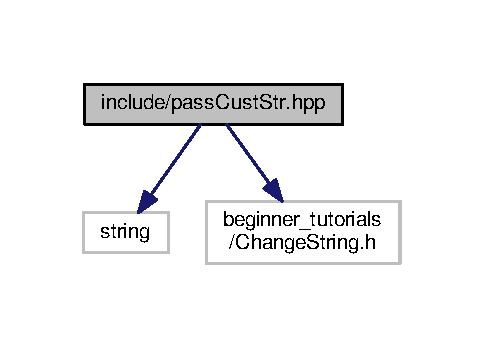
\includegraphics[width=232pt]{passCustStr_8hpp__incl}
\end{center}
\end{figure}
This graph shows which files directly or indirectly include this file\+:\nopagebreak
\begin{figure}[H]
\begin{center}
\leavevmode
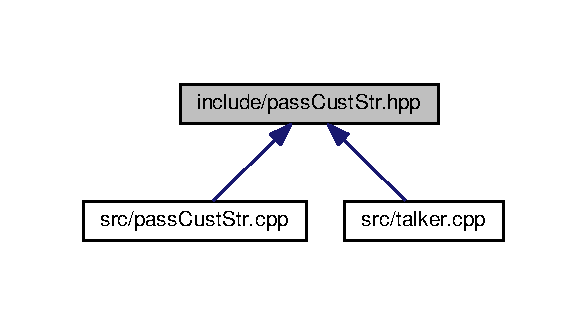
\includegraphics[width=282pt]{passCustStr_8hpp__dep__incl}
\end{center}
\end{figure}
\subsection*{Classes}
\begin{DoxyCompactItemize}
\item 
class \hyperlink{classpassCustStr}{pass\+Cust\+Str}
\end{DoxyCompactItemize}

\hypertarget{license_8txt}{}\section{license.\+txt File Reference}
\label{license_8txt}\index{license.\+txt@{license.\+txt}}
\subsection*{Functions}
\begin{DoxyCompactItemize}
\item 
Copyright Yuyu\+Hsueh Redistribution and use in source and binary with or without are permitted provided that the following conditions are this list of conditions and the following disclaimer Redistributions in binary form must reproduce the above copyright this list of conditions and the following disclaimer in the documentation and or other materials provided with the distribution Neither the name of the copyright holder nor the names of its contributors may be used to endorse or promote products derived from this software without specific prior written permission T\+H\+IS S\+O\+F\+T\+W\+A\+RE IS P\+R\+O\+V\+I\+D\+ED BY T\+HE C\+O\+P\+Y\+R\+I\+G\+HT H\+O\+L\+D\+E\+RS A\+ND C\+O\+N\+T\+R\+I\+B\+U\+T\+O\+RS AS IS A\+ND A\+NY E\+X\+P\+R\+E\+SS OR I\+M\+P\+L\+I\+ED B\+UT N\+OT L\+I\+M\+I\+T\+ED T\+HE I\+M\+P\+L\+I\+ED \hyperlink{license_8txt_a042eb66328050ad88743187ae8e43b95}{W\+A\+R\+R\+A\+N\+T\+I\+ES} OF M\+E\+R\+C\+H\+A\+N\+T\+A\+B\+I\+L\+I\+TY A\+ND F\+I\+T\+N\+E\+SS F\+OR A P\+A\+R\+T\+I\+C\+U\+L\+AR P\+U\+R\+P\+O\+SE A\+RE D\+I\+S\+C\+L\+A\+I\+M\+ED IN NO E\+V\+E\+NT S\+H\+A\+LL T\+HE C\+O\+P\+Y\+R\+I\+G\+HT H\+O\+L\+D\+ER OR C\+O\+N\+T\+R\+I\+B\+U\+T\+O\+RS BE L\+I\+A\+B\+LE F\+OR A\+NY OR C\+O\+N\+S\+E\+Q\+U\+E\+N\+T\+I\+AL \hyperlink{license_8txt_aef6a70d7e2ff0800bdd6b6c943108868}{D\+A\+M\+A\+G\+ES} (\hyperlink{license_8txt_ac6699313e23a90e93d8db75154e2e689}{I\+N\+C\+L\+U\+D\+I\+NG}, B\+UT N\+OT L\+I\+M\+I\+T\+ED \hyperlink{license_8txt_a4bddb9a7dc45727be85d1869ee6c870d}{TO}, P\+R\+O\+C\+U\+R\+E\+M\+E\+NT OF S\+U\+B\+S\+T\+I\+T\+U\+TE G\+O\+O\+DS OR S\+E\+R\+V\+I\+C\+ES;L\+O\+SS OF U\+SE, D\+A\+TA, OR P\+R\+O\+F\+I\+TS;OR B\+U\+S\+I\+N\+E\+SS I\+N\+T\+E\+R\+R\+U\+P\+T\+I\+ON) H\+O\+W\+E\+V\+ER C\+A\+U\+S\+ED A\+ND ON A\+NY T\+H\+E\+O\+RY OF \hyperlink{license_8txt_a293cddb201641aed1186322968630e55}{L\+I\+A\+B\+I\+L\+I\+TY}
\item 
Copyright Yuyu\+Hsueh Redistribution and use in source and binary with or without are permitted provided that the following conditions are this list of conditions and the following disclaimer Redistributions in binary form must reproduce the above copyright this list of conditions and the following disclaimer in the documentation and or other materials provided with the distribution Neither the name of the copyright holder nor the names of its contributors may be used to endorse or promote products derived from this software without specific prior written permission T\+H\+IS S\+O\+F\+T\+W\+A\+RE IS P\+R\+O\+V\+I\+D\+ED BY T\+HE C\+O\+P\+Y\+R\+I\+G\+HT H\+O\+L\+D\+E\+RS A\+ND C\+O\+N\+T\+R\+I\+B\+U\+T\+O\+RS AS IS A\+ND A\+NY E\+X\+P\+R\+E\+SS OR I\+M\+P\+L\+I\+ED B\+UT N\+OT L\+I\+M\+I\+T\+ED T\+HE I\+M\+P\+L\+I\+ED \hyperlink{license_8txt_a042eb66328050ad88743187ae8e43b95}{W\+A\+R\+R\+A\+N\+T\+I\+ES} OF M\+E\+R\+C\+H\+A\+N\+T\+A\+B\+I\+L\+I\+TY A\+ND F\+I\+T\+N\+E\+SS F\+OR A P\+A\+R\+T\+I\+C\+U\+L\+AR P\+U\+R\+P\+O\+SE A\+RE D\+I\+S\+C\+L\+A\+I\+M\+ED IN NO E\+V\+E\+NT S\+H\+A\+LL T\+HE C\+O\+P\+Y\+R\+I\+G\+HT H\+O\+L\+D\+ER OR C\+O\+N\+T\+R\+I\+B\+U\+T\+O\+RS BE L\+I\+A\+B\+LE F\+OR A\+NY OR C\+O\+N\+S\+E\+Q\+U\+E\+N\+T\+I\+AL W\+H\+E\+T\+H\+ER IN S\+T\+R\+I\+CT OR \hyperlink{license_8txt_a053f3866e9a0ed6d815ff119b776cf19}{T\+O\+RT} (\hyperlink{license_8txt_ac6699313e23a90e93d8db75154e2e689}{I\+N\+C\+L\+U\+D\+I\+NG} N\+E\+G\+L\+I\+G\+E\+N\+CE OR O\+T\+H\+E\+R\+W\+I\+SE) A\+R\+I\+S\+I\+NG IN A\+NY W\+AY O\+UT OF T\+HE U\+SE OF T\+H\+IS S\+O\+F\+T\+W\+A\+RE
\end{DoxyCompactItemize}
\subsection*{Variables}
\begin{DoxyCompactItemize}
\item 
Copyright Yuyu\+Hsueh Redistribution and use in source and binary \hyperlink{license_8txt_a907462b7b3ae0a9072f23e05f66fb7f1}{forms}
\item 
Copyright Yuyu\+Hsueh Redistribution and use in source and binary with or without \hyperlink{license_8txt_ad26192e5b2b1fdec8883d2c0110e35c6}{modification}
\item 
Copyright Yuyu\+Hsueh Redistribution and use in source and binary with or without are permitted provided that the following conditions are \hyperlink{license_8txt_ac8582a50364a60dd4d7d7d24f725c413}{met}
\item 
Copyright Yuyu\+Hsueh Redistribution and use in source and binary with or without are permitted provided that the following conditions are this list of conditions and the following disclaimer Redistributions in binary form must reproduce the above copyright \hyperlink{license_8txt_af4bbea5cb99610e4ef2a43c12b41e9c9}{notice}
\item 
Copyright Yuyu\+Hsueh Redistribution and use in source and binary with or without are permitted provided that the following conditions are this list of conditions and the following disclaimer Redistributions in binary form must reproduce the above copyright this list of conditions and the following disclaimer in the documentation and or other materials provided with the distribution Neither the name of the copyright holder nor the names of its contributors may be used to endorse or promote products derived from this software without specific prior written permission T\+H\+IS S\+O\+F\+T\+W\+A\+RE IS P\+R\+O\+V\+I\+D\+ED BY T\+HE C\+O\+P\+Y\+R\+I\+G\+HT H\+O\+L\+D\+E\+RS A\+ND C\+O\+N\+T\+R\+I\+B\+U\+T\+O\+RS AS IS A\+ND A\+NY E\+X\+P\+R\+E\+SS OR I\+M\+P\+L\+I\+ED \hyperlink{license_8txt_a042eb66328050ad88743187ae8e43b95}{W\+A\+R\+R\+A\+N\+T\+I\+ES}
\item 
Copyright Yuyu\+Hsueh Redistribution and use in source and binary with or without are permitted provided that the following conditions are this list of conditions and the following disclaimer Redistributions in binary form must reproduce the above copyright this list of conditions and the following disclaimer in the documentation and or other materials provided with the distribution Neither the name of the copyright holder nor the names of its contributors may be used to endorse or promote products derived from this software without specific prior written permission T\+H\+IS S\+O\+F\+T\+W\+A\+RE IS P\+R\+O\+V\+I\+D\+ED BY T\+HE C\+O\+P\+Y\+R\+I\+G\+HT H\+O\+L\+D\+E\+RS A\+ND C\+O\+N\+T\+R\+I\+B\+U\+T\+O\+RS AS IS A\+ND A\+NY E\+X\+P\+R\+E\+SS OR I\+M\+P\+L\+I\+ED \hyperlink{license_8txt_ac6699313e23a90e93d8db75154e2e689}{I\+N\+C\+L\+U\+D\+I\+NG}
\item 
Copyright Yuyu\+Hsueh Redistribution and use in source and binary with or without are permitted provided that the following conditions are this list of conditions and the following disclaimer Redistributions in binary form must reproduce the above copyright this list of conditions and the following disclaimer in the documentation and or other materials provided with the distribution Neither the name of the copyright holder nor the names of its contributors may be used to endorse or promote products derived from this software without specific prior written permission T\+H\+IS S\+O\+F\+T\+W\+A\+RE IS P\+R\+O\+V\+I\+D\+ED BY T\+HE C\+O\+P\+Y\+R\+I\+G\+HT H\+O\+L\+D\+E\+RS A\+ND C\+O\+N\+T\+R\+I\+B\+U\+T\+O\+RS AS IS A\+ND A\+NY E\+X\+P\+R\+E\+SS OR I\+M\+P\+L\+I\+ED B\+UT N\+OT L\+I\+M\+I\+T\+ED \hyperlink{license_8txt_a4bddb9a7dc45727be85d1869ee6c870d}{TO}
\item 
Copyright Yuyu\+Hsueh Redistribution and use in source and binary with or without are permitted provided that the following conditions are this list of conditions and the following disclaimer Redistributions in binary form must reproduce the above copyright this list of conditions and the following disclaimer in the documentation and or other materials provided with the distribution Neither the name of the copyright holder nor the names of its contributors may be used to endorse or promote products derived from this software without specific prior written permission T\+H\+IS S\+O\+F\+T\+W\+A\+RE IS P\+R\+O\+V\+I\+D\+ED BY T\+HE C\+O\+P\+Y\+R\+I\+G\+HT H\+O\+L\+D\+E\+RS A\+ND C\+O\+N\+T\+R\+I\+B\+U\+T\+O\+RS AS IS A\+ND A\+NY E\+X\+P\+R\+E\+SS OR I\+M\+P\+L\+I\+ED B\+UT N\+OT L\+I\+M\+I\+T\+ED T\+HE I\+M\+P\+L\+I\+ED \hyperlink{license_8txt_a042eb66328050ad88743187ae8e43b95}{W\+A\+R\+R\+A\+N\+T\+I\+ES} OF M\+E\+R\+C\+H\+A\+N\+T\+A\+B\+I\+L\+I\+TY A\+ND F\+I\+T\+N\+E\+SS F\+OR A P\+A\+R\+T\+I\+C\+U\+L\+AR P\+U\+R\+P\+O\+SE A\+RE D\+I\+S\+C\+L\+A\+I\+M\+ED IN NO E\+V\+E\+NT S\+H\+A\+LL T\+HE C\+O\+P\+Y\+R\+I\+G\+HT H\+O\+L\+D\+ER OR C\+O\+N\+T\+R\+I\+B\+U\+T\+O\+RS BE L\+I\+A\+B\+LE F\+OR A\+NY \hyperlink{license_8txt_a9ecfdaf89f3cf85421feb43ef16f372d}{D\+I\+R\+E\+CT}
\item 
Copyright Yuyu\+Hsueh Redistribution and use in source and binary with or without are permitted provided that the following conditions are this list of conditions and the following disclaimer Redistributions in binary form must reproduce the above copyright this list of conditions and the following disclaimer in the documentation and or other materials provided with the distribution Neither the name of the copyright holder nor the names of its contributors may be used to endorse or promote products derived from this software without specific prior written permission T\+H\+IS S\+O\+F\+T\+W\+A\+RE IS P\+R\+O\+V\+I\+D\+ED BY T\+HE C\+O\+P\+Y\+R\+I\+G\+HT H\+O\+L\+D\+E\+RS A\+ND C\+O\+N\+T\+R\+I\+B\+U\+T\+O\+RS AS IS A\+ND A\+NY E\+X\+P\+R\+E\+SS OR I\+M\+P\+L\+I\+ED B\+UT N\+OT L\+I\+M\+I\+T\+ED T\+HE I\+M\+P\+L\+I\+ED \hyperlink{license_8txt_a042eb66328050ad88743187ae8e43b95}{W\+A\+R\+R\+A\+N\+T\+I\+ES} OF M\+E\+R\+C\+H\+A\+N\+T\+A\+B\+I\+L\+I\+TY A\+ND F\+I\+T\+N\+E\+SS F\+OR A P\+A\+R\+T\+I\+C\+U\+L\+AR P\+U\+R\+P\+O\+SE A\+RE D\+I\+S\+C\+L\+A\+I\+M\+ED IN NO E\+V\+E\+NT S\+H\+A\+LL T\+HE C\+O\+P\+Y\+R\+I\+G\+HT H\+O\+L\+D\+ER OR C\+O\+N\+T\+R\+I\+B\+U\+T\+O\+RS BE L\+I\+A\+B\+LE F\+OR A\+NY \hyperlink{license_8txt_a8c44c311e30c2c13cd7035f237993b51}{I\+N\+D\+I\+R\+E\+CT}
\item 
Copyright Yuyu\+Hsueh Redistribution and use in source and binary with or without are permitted provided that the following conditions are this list of conditions and the following disclaimer Redistributions in binary form must reproduce the above copyright this list of conditions and the following disclaimer in the documentation and or other materials provided with the distribution Neither the name of the copyright holder nor the names of its contributors may be used to endorse or promote products derived from this software without specific prior written permission T\+H\+IS S\+O\+F\+T\+W\+A\+RE IS P\+R\+O\+V\+I\+D\+ED BY T\+HE C\+O\+P\+Y\+R\+I\+G\+HT H\+O\+L\+D\+E\+RS A\+ND C\+O\+N\+T\+R\+I\+B\+U\+T\+O\+RS AS IS A\+ND A\+NY E\+X\+P\+R\+E\+SS OR I\+M\+P\+L\+I\+ED B\+UT N\+OT L\+I\+M\+I\+T\+ED T\+HE I\+M\+P\+L\+I\+ED \hyperlink{license_8txt_a042eb66328050ad88743187ae8e43b95}{W\+A\+R\+R\+A\+N\+T\+I\+ES} OF M\+E\+R\+C\+H\+A\+N\+T\+A\+B\+I\+L\+I\+TY A\+ND F\+I\+T\+N\+E\+SS F\+OR A P\+A\+R\+T\+I\+C\+U\+L\+AR P\+U\+R\+P\+O\+SE A\+RE D\+I\+S\+C\+L\+A\+I\+M\+ED IN NO E\+V\+E\+NT S\+H\+A\+LL T\+HE C\+O\+P\+Y\+R\+I\+G\+HT H\+O\+L\+D\+ER OR C\+O\+N\+T\+R\+I\+B\+U\+T\+O\+RS BE L\+I\+A\+B\+LE F\+OR A\+NY \hyperlink{license_8txt_a6fe13299500a9a6c4af4434723e6afae}{I\+N\+C\+I\+D\+E\+N\+T\+AL}
\item 
Copyright Yuyu\+Hsueh Redistribution and use in source and binary with or without are permitted provided that the following conditions are this list of conditions and the following disclaimer Redistributions in binary form must reproduce the above copyright this list of conditions and the following disclaimer in the documentation and or other materials provided with the distribution Neither the name of the copyright holder nor the names of its contributors may be used to endorse or promote products derived from this software without specific prior written permission T\+H\+IS S\+O\+F\+T\+W\+A\+RE IS P\+R\+O\+V\+I\+D\+ED BY T\+HE C\+O\+P\+Y\+R\+I\+G\+HT H\+O\+L\+D\+E\+RS A\+ND C\+O\+N\+T\+R\+I\+B\+U\+T\+O\+RS AS IS A\+ND A\+NY E\+X\+P\+R\+E\+SS OR I\+M\+P\+L\+I\+ED B\+UT N\+OT L\+I\+M\+I\+T\+ED T\+HE I\+M\+P\+L\+I\+ED \hyperlink{license_8txt_a042eb66328050ad88743187ae8e43b95}{W\+A\+R\+R\+A\+N\+T\+I\+ES} OF M\+E\+R\+C\+H\+A\+N\+T\+A\+B\+I\+L\+I\+TY A\+ND F\+I\+T\+N\+E\+SS F\+OR A P\+A\+R\+T\+I\+C\+U\+L\+AR P\+U\+R\+P\+O\+SE A\+RE D\+I\+S\+C\+L\+A\+I\+M\+ED IN NO E\+V\+E\+NT S\+H\+A\+LL T\+HE C\+O\+P\+Y\+R\+I\+G\+HT H\+O\+L\+D\+ER OR C\+O\+N\+T\+R\+I\+B\+U\+T\+O\+RS BE L\+I\+A\+B\+LE F\+OR A\+NY \hyperlink{license_8txt_a910ad17f295c48bc77c8ee2434bf4ac5}{S\+P\+E\+C\+I\+AL}
\item 
Copyright Yuyu\+Hsueh Redistribution and use in source and binary with or without are permitted provided that the following conditions are this list of conditions and the following disclaimer Redistributions in binary form must reproduce the above copyright this list of conditions and the following disclaimer in the documentation and or other materials provided with the distribution Neither the name of the copyright holder nor the names of its contributors may be used to endorse or promote products derived from this software without specific prior written permission T\+H\+IS S\+O\+F\+T\+W\+A\+RE IS P\+R\+O\+V\+I\+D\+ED BY T\+HE C\+O\+P\+Y\+R\+I\+G\+HT H\+O\+L\+D\+E\+RS A\+ND C\+O\+N\+T\+R\+I\+B\+U\+T\+O\+RS AS IS A\+ND A\+NY E\+X\+P\+R\+E\+SS OR I\+M\+P\+L\+I\+ED B\+UT N\+OT L\+I\+M\+I\+T\+ED T\+HE I\+M\+P\+L\+I\+ED \hyperlink{license_8txt_a042eb66328050ad88743187ae8e43b95}{W\+A\+R\+R\+A\+N\+T\+I\+ES} OF M\+E\+R\+C\+H\+A\+N\+T\+A\+B\+I\+L\+I\+TY A\+ND F\+I\+T\+N\+E\+SS F\+OR A P\+A\+R\+T\+I\+C\+U\+L\+AR P\+U\+R\+P\+O\+SE A\+RE D\+I\+S\+C\+L\+A\+I\+M\+ED IN NO E\+V\+E\+NT S\+H\+A\+LL T\+HE C\+O\+P\+Y\+R\+I\+G\+HT H\+O\+L\+D\+ER OR C\+O\+N\+T\+R\+I\+B\+U\+T\+O\+RS BE L\+I\+A\+B\+LE F\+OR A\+NY \hyperlink{license_8txt_ac4a6acd1ced6bfbf36f00e4629d74515}{E\+X\+E\+M\+P\+L\+A\+RY}
\item 
Copyright Yuyu\+Hsueh Redistribution and use in source and binary with or without are permitted provided that the following conditions are this list of conditions and the following disclaimer Redistributions in binary form must reproduce the above copyright this list of conditions and the following disclaimer in the documentation and or other materials provided with the distribution Neither the name of the copyright holder nor the names of its contributors may be used to endorse or promote products derived from this software without specific prior written permission T\+H\+IS S\+O\+F\+T\+W\+A\+RE IS P\+R\+O\+V\+I\+D\+ED BY T\+HE C\+O\+P\+Y\+R\+I\+G\+HT H\+O\+L\+D\+E\+RS A\+ND C\+O\+N\+T\+R\+I\+B\+U\+T\+O\+RS AS IS A\+ND A\+NY E\+X\+P\+R\+E\+SS OR I\+M\+P\+L\+I\+ED B\+UT N\+OT L\+I\+M\+I\+T\+ED T\+HE I\+M\+P\+L\+I\+ED \hyperlink{license_8txt_a042eb66328050ad88743187ae8e43b95}{W\+A\+R\+R\+A\+N\+T\+I\+ES} OF M\+E\+R\+C\+H\+A\+N\+T\+A\+B\+I\+L\+I\+TY A\+ND F\+I\+T\+N\+E\+SS F\+OR A P\+A\+R\+T\+I\+C\+U\+L\+AR P\+U\+R\+P\+O\+SE A\+RE D\+I\+S\+C\+L\+A\+I\+M\+ED IN NO E\+V\+E\+NT S\+H\+A\+LL T\+HE C\+O\+P\+Y\+R\+I\+G\+HT H\+O\+L\+D\+ER OR C\+O\+N\+T\+R\+I\+B\+U\+T\+O\+RS BE L\+I\+A\+B\+LE F\+OR A\+NY OR C\+O\+N\+S\+E\+Q\+U\+E\+N\+T\+I\+AL W\+H\+E\+T\+H\+ER IN \hyperlink{license_8txt_ad1b3910f726d03f8987a2ad1665d309c}{C\+O\+N\+T\+R\+A\+CT}
\item 
Copyright Yuyu\+Hsueh Redistribution and use in source and binary with or without are permitted provided that the following conditions are this list of conditions and the following disclaimer Redistributions in binary form must reproduce the above copyright this list of conditions and the following disclaimer in the documentation and or other materials provided with the distribution Neither the name of the copyright holder nor the names of its contributors may be used to endorse or promote products derived from this software without specific prior written permission T\+H\+IS S\+O\+F\+T\+W\+A\+RE IS P\+R\+O\+V\+I\+D\+ED BY T\+HE C\+O\+P\+Y\+R\+I\+G\+HT H\+O\+L\+D\+E\+RS A\+ND C\+O\+N\+T\+R\+I\+B\+U\+T\+O\+RS AS IS A\+ND A\+NY E\+X\+P\+R\+E\+SS OR I\+M\+P\+L\+I\+ED B\+UT N\+OT L\+I\+M\+I\+T\+ED T\+HE I\+M\+P\+L\+I\+ED \hyperlink{license_8txt_a042eb66328050ad88743187ae8e43b95}{W\+A\+R\+R\+A\+N\+T\+I\+ES} OF M\+E\+R\+C\+H\+A\+N\+T\+A\+B\+I\+L\+I\+TY A\+ND F\+I\+T\+N\+E\+SS F\+OR A P\+A\+R\+T\+I\+C\+U\+L\+AR P\+U\+R\+P\+O\+SE A\+RE D\+I\+S\+C\+L\+A\+I\+M\+ED IN NO E\+V\+E\+NT S\+H\+A\+LL T\+HE C\+O\+P\+Y\+R\+I\+G\+HT H\+O\+L\+D\+ER OR C\+O\+N\+T\+R\+I\+B\+U\+T\+O\+RS BE L\+I\+A\+B\+LE F\+OR A\+NY OR C\+O\+N\+S\+E\+Q\+U\+E\+N\+T\+I\+AL W\+H\+E\+T\+H\+ER IN S\+T\+R\+I\+CT \hyperlink{license_8txt_a293cddb201641aed1186322968630e55}{L\+I\+A\+B\+I\+L\+I\+TY}
\end{DoxyCompactItemize}


\subsection{Function Documentation}
\index{license.\+txt@{license.\+txt}!D\+A\+M\+A\+G\+ES@{D\+A\+M\+A\+G\+ES}}
\index{D\+A\+M\+A\+G\+ES@{D\+A\+M\+A\+G\+ES}!license.\+txt@{license.\+txt}}
\subsubsection[{\texorpdfstring{D\+A\+M\+A\+G\+E\+S(\+I\+N\+C\+L\+U\+D\+I\+N\+G, B\+U\+T N\+O\+T L\+I\+M\+I\+T\+E\+D T\+O, P\+R\+O\+C\+U\+R\+E\+M\+E\+N\+T O\+F S\+U\+B\+S\+T\+I\+T\+U\+T\+E G\+O\+O\+D\+S O\+R S\+E\+R\+V\+I\+C\+E\+S;\+L\+O\+S\+S O\+F U\+S\+E, D\+A\+T\+A, O\+R P\+R\+O\+F\+I\+T\+S;\+O\+R B\+U\+S\+I\+N\+E\+S\+S I\+N\+T\+E\+R\+R\+U\+P\+T\+I\+O\+N) H\+O\+W\+E\+V\+E\+R C\+A\+U\+S\+E\+D A\+N\+D O\+N A\+N\+Y T\+H\+E\+O\+R\+Y O\+F L\+I\+A\+B\+I\+L\+I\+TY}{DAMAGES(INCLUDING, BUT NOT LIMITED TO, PROCUREMENT OF SUBSTITUTE GOODS OR SERVICES;LOSS OF USE, DATA, OR PROFITS;OR BUSINESS INTERRUPTION) HOWEVER CAUSED AND ON ANY THEORY OF LIABILITY}}]{\setlength{\rightskip}{0pt plus 5cm}Copyright Yuyu\+Hsueh Redistribution and use in source and binary with or without are permitted provided that the following conditions are this list of conditions and the following disclaimer Redistributions in binary form must reproduce the above copyright this list of conditions and the following disclaimer in the documentation and or other materials provided with the distribution Neither the name of the copyright holder nor the names of its contributors may be used to endorse or promote products derived from this software without specific prior written permission T\+H\+IS S\+O\+F\+T\+W\+A\+RE IS P\+R\+O\+V\+I\+D\+ED BY T\+HE C\+O\+P\+Y\+R\+I\+G\+HT H\+O\+L\+D\+E\+RS A\+ND C\+O\+N\+T\+R\+I\+B\+U\+T\+O\+RS AS IS A\+ND A\+NY E\+X\+P\+R\+E\+SS OR I\+M\+P\+L\+I\+ED B\+UT N\+OT L\+I\+M\+I\+T\+ED T\+HE I\+M\+P\+L\+I\+ED {\bf W\+A\+R\+R\+A\+N\+T\+I\+ES} OF M\+E\+R\+C\+H\+A\+N\+T\+A\+B\+I\+L\+I\+TY A\+ND F\+I\+T\+N\+E\+SS F\+OR A P\+A\+R\+T\+I\+C\+U\+L\+AR P\+U\+R\+P\+O\+SE A\+RE D\+I\+S\+C\+L\+A\+I\+M\+ED IN NO E\+V\+E\+NT S\+H\+A\+LL T\+HE C\+O\+P\+Y\+R\+I\+G\+HT H\+O\+L\+D\+ER OR C\+O\+N\+T\+R\+I\+B\+U\+T\+O\+RS BE L\+I\+A\+B\+LE F\+OR A\+NY OR C\+O\+N\+S\+E\+Q\+U\+E\+N\+T\+I\+AL D\+A\+M\+A\+G\+ES (
\begin{DoxyParamCaption}
\item[{{\bf I\+N\+C\+L\+U\+D\+I\+NG}}]{, }
\item[{B\+UT N\+OT L\+I\+M\+I\+T\+ED}]{TO, }
\item[{P\+R\+O\+C\+U\+R\+E\+M\+E\+NT OF S\+U\+B\+S\+T\+I\+T\+U\+TE G\+O\+O\+DS OR S\+E\+R\+V\+I\+C\+ES;L\+O\+SS OF}]{U\+SE, }
\item[{D\+A\+TA}]{, }
\item[{OR P\+R\+O\+F\+I\+TS;OR B\+U\+S\+I\+N\+E\+SS}]{I\+N\+T\+E\+R\+R\+U\+P\+T\+I\+ON}
\end{DoxyParamCaption}
)}\hypertarget{license_8txt_aef6a70d7e2ff0800bdd6b6c943108868}{}\label{license_8txt_aef6a70d7e2ff0800bdd6b6c943108868}
\index{license.\+txt@{license.\+txt}!T\+O\+RT@{T\+O\+RT}}
\index{T\+O\+RT@{T\+O\+RT}!license.\+txt@{license.\+txt}}
\subsubsection[{\texorpdfstring{T\+O\+R\+T(\+I\+N\+C\+L\+U\+D\+I\+N\+G N\+E\+G\+L\+I\+G\+E\+N\+C\+E O\+R O\+T\+H\+E\+R\+W\+I\+S\+E) A\+R\+I\+S\+I\+N\+G I\+N A\+N\+Y W\+A\+Y O\+U\+T O\+F T\+H\+E U\+S\+E O\+F T\+H\+I\+S S\+O\+F\+T\+W\+A\+RE}{TORT(INCLUDING NEGLIGENCE OR OTHERWISE) ARISING IN ANY WAY OUT OF THE USE OF THIS SOFTWARE}}]{\setlength{\rightskip}{0pt plus 5cm}Copyright Yuyu\+Hsueh Redistribution and use in source and binary with or without are permitted provided that the following conditions are this list of conditions and the following disclaimer Redistributions in binary form must reproduce the above copyright this list of conditions and the following disclaimer in the documentation and or other materials provided with the distribution Neither the name of the copyright holder nor the names of its contributors may be used to endorse or promote products derived from this software without specific prior written permission T\+H\+IS S\+O\+F\+T\+W\+A\+RE IS P\+R\+O\+V\+I\+D\+ED BY T\+HE C\+O\+P\+Y\+R\+I\+G\+HT H\+O\+L\+D\+E\+RS A\+ND C\+O\+N\+T\+R\+I\+B\+U\+T\+O\+RS AS IS A\+ND A\+NY E\+X\+P\+R\+E\+SS OR I\+M\+P\+L\+I\+ED B\+UT N\+OT L\+I\+M\+I\+T\+ED T\+HE I\+M\+P\+L\+I\+ED {\bf W\+A\+R\+R\+A\+N\+T\+I\+ES} OF M\+E\+R\+C\+H\+A\+N\+T\+A\+B\+I\+L\+I\+TY A\+ND F\+I\+T\+N\+E\+SS F\+OR A P\+A\+R\+T\+I\+C\+U\+L\+AR P\+U\+R\+P\+O\+SE A\+RE D\+I\+S\+C\+L\+A\+I\+M\+ED IN NO E\+V\+E\+NT S\+H\+A\+LL T\+HE C\+O\+P\+Y\+R\+I\+G\+HT H\+O\+L\+D\+ER OR C\+O\+N\+T\+R\+I\+B\+U\+T\+O\+RS BE L\+I\+A\+B\+LE F\+OR A\+NY OR C\+O\+N\+S\+E\+Q\+U\+E\+N\+T\+I\+AL W\+H\+E\+T\+H\+ER IN S\+T\+R\+I\+CT OR T\+O\+RT (
\begin{DoxyParamCaption}
\item[{{\bf I\+N\+C\+L\+U\+D\+I\+NG} N\+E\+G\+L\+I\+G\+E\+N\+CE OR}]{O\+T\+H\+E\+R\+W\+I\+SE}
\end{DoxyParamCaption}
)}\hypertarget{license_8txt_a053f3866e9a0ed6d815ff119b776cf19}{}\label{license_8txt_a053f3866e9a0ed6d815ff119b776cf19}


\subsection{Variable Documentation}
\index{license.\+txt@{license.\+txt}!C\+O\+N\+T\+R\+A\+CT@{C\+O\+N\+T\+R\+A\+CT}}
\index{C\+O\+N\+T\+R\+A\+CT@{C\+O\+N\+T\+R\+A\+CT}!license.\+txt@{license.\+txt}}
\subsubsection[{\texorpdfstring{C\+O\+N\+T\+R\+A\+CT}{CONTRACT}}]{\setlength{\rightskip}{0pt plus 5cm}Copyright Yuyu\+Hsueh Redistribution and use in source and binary with or without are permitted provided that the following conditions are this list of conditions and the following disclaimer Redistributions in binary form must reproduce the above copyright this list of conditions and the following disclaimer in the documentation and or other materials provided with the distribution Neither the name of the copyright holder nor the names of its contributors may be used to endorse or promote products derived from this software without specific prior written permission T\+H\+IS S\+O\+F\+T\+W\+A\+RE IS P\+R\+O\+V\+I\+D\+ED BY T\+HE C\+O\+P\+Y\+R\+I\+G\+HT H\+O\+L\+D\+E\+RS A\+ND C\+O\+N\+T\+R\+I\+B\+U\+T\+O\+RS AS IS A\+ND A\+NY E\+X\+P\+R\+E\+SS OR I\+M\+P\+L\+I\+ED B\+UT N\+OT L\+I\+M\+I\+T\+ED T\+HE I\+M\+P\+L\+I\+ED {\bf W\+A\+R\+R\+A\+N\+T\+I\+ES} OF M\+E\+R\+C\+H\+A\+N\+T\+A\+B\+I\+L\+I\+TY A\+ND F\+I\+T\+N\+E\+SS F\+OR A P\+A\+R\+T\+I\+C\+U\+L\+AR P\+U\+R\+P\+O\+SE A\+RE D\+I\+S\+C\+L\+A\+I\+M\+ED IN NO E\+V\+E\+NT S\+H\+A\+LL T\+HE C\+O\+P\+Y\+R\+I\+G\+HT H\+O\+L\+D\+ER OR C\+O\+N\+T\+R\+I\+B\+U\+T\+O\+RS BE L\+I\+A\+B\+LE F\+OR A\+NY OR C\+O\+N\+S\+E\+Q\+U\+E\+N\+T\+I\+AL W\+H\+E\+T\+H\+ER IN C\+O\+N\+T\+R\+A\+CT}\hypertarget{license_8txt_ad1b3910f726d03f8987a2ad1665d309c}{}\label{license_8txt_ad1b3910f726d03f8987a2ad1665d309c}
\index{license.\+txt@{license.\+txt}!D\+I\+R\+E\+CT@{D\+I\+R\+E\+CT}}
\index{D\+I\+R\+E\+CT@{D\+I\+R\+E\+CT}!license.\+txt@{license.\+txt}}
\subsubsection[{\texorpdfstring{D\+I\+R\+E\+CT}{DIRECT}}]{\setlength{\rightskip}{0pt plus 5cm}Copyright Yuyu\+Hsueh Redistribution and use in source and binary with or without are permitted provided that the following conditions are this list of conditions and the following disclaimer Redistributions in binary form must reproduce the above copyright this list of conditions and the following disclaimer in the documentation and or other materials provided with the distribution Neither the name of the copyright holder nor the names of its contributors may be used to endorse or promote products derived from this software without specific prior written permission T\+H\+IS S\+O\+F\+T\+W\+A\+RE IS P\+R\+O\+V\+I\+D\+ED BY T\+HE C\+O\+P\+Y\+R\+I\+G\+HT H\+O\+L\+D\+E\+RS A\+ND C\+O\+N\+T\+R\+I\+B\+U\+T\+O\+RS AS IS A\+ND A\+NY E\+X\+P\+R\+E\+SS OR I\+M\+P\+L\+I\+ED B\+UT N\+OT L\+I\+M\+I\+T\+ED T\+HE I\+M\+P\+L\+I\+ED {\bf W\+A\+R\+R\+A\+N\+T\+I\+ES} OF M\+E\+R\+C\+H\+A\+N\+T\+A\+B\+I\+L\+I\+TY A\+ND F\+I\+T\+N\+E\+SS F\+OR A P\+A\+R\+T\+I\+C\+U\+L\+AR P\+U\+R\+P\+O\+SE A\+RE D\+I\+S\+C\+L\+A\+I\+M\+ED IN NO E\+V\+E\+NT S\+H\+A\+LL T\+HE C\+O\+P\+Y\+R\+I\+G\+HT H\+O\+L\+D\+ER OR C\+O\+N\+T\+R\+I\+B\+U\+T\+O\+RS BE L\+I\+A\+B\+LE F\+OR A\+NY D\+I\+R\+E\+CT}\hypertarget{license_8txt_a9ecfdaf89f3cf85421feb43ef16f372d}{}\label{license_8txt_a9ecfdaf89f3cf85421feb43ef16f372d}
\index{license.\+txt@{license.\+txt}!E\+X\+E\+M\+P\+L\+A\+RY@{E\+X\+E\+M\+P\+L\+A\+RY}}
\index{E\+X\+E\+M\+P\+L\+A\+RY@{E\+X\+E\+M\+P\+L\+A\+RY}!license.\+txt@{license.\+txt}}
\subsubsection[{\texorpdfstring{E\+X\+E\+M\+P\+L\+A\+RY}{EXEMPLARY}}]{\setlength{\rightskip}{0pt plus 5cm}Copyright Yuyu\+Hsueh Redistribution and use in source and binary with or without are permitted provided that the following conditions are this list of conditions and the following disclaimer Redistributions in binary form must reproduce the above copyright this list of conditions and the following disclaimer in the documentation and or other materials provided with the distribution Neither the name of the copyright holder nor the names of its contributors may be used to endorse or promote products derived from this software without specific prior written permission T\+H\+IS S\+O\+F\+T\+W\+A\+RE IS P\+R\+O\+V\+I\+D\+ED BY T\+HE C\+O\+P\+Y\+R\+I\+G\+HT H\+O\+L\+D\+E\+RS A\+ND C\+O\+N\+T\+R\+I\+B\+U\+T\+O\+RS AS IS A\+ND A\+NY E\+X\+P\+R\+E\+SS OR I\+M\+P\+L\+I\+ED B\+UT N\+OT L\+I\+M\+I\+T\+ED T\+HE I\+M\+P\+L\+I\+ED {\bf W\+A\+R\+R\+A\+N\+T\+I\+ES} OF M\+E\+R\+C\+H\+A\+N\+T\+A\+B\+I\+L\+I\+TY A\+ND F\+I\+T\+N\+E\+SS F\+OR A P\+A\+R\+T\+I\+C\+U\+L\+AR P\+U\+R\+P\+O\+SE A\+RE D\+I\+S\+C\+L\+A\+I\+M\+ED IN NO E\+V\+E\+NT S\+H\+A\+LL T\+HE C\+O\+P\+Y\+R\+I\+G\+HT H\+O\+L\+D\+ER OR C\+O\+N\+T\+R\+I\+B\+U\+T\+O\+RS BE L\+I\+A\+B\+LE F\+OR A\+NY E\+X\+E\+M\+P\+L\+A\+RY}\hypertarget{license_8txt_ac4a6acd1ced6bfbf36f00e4629d74515}{}\label{license_8txt_ac4a6acd1ced6bfbf36f00e4629d74515}
\index{license.\+txt@{license.\+txt}!forms@{forms}}
\index{forms@{forms}!license.\+txt@{license.\+txt}}
\subsubsection[{\texorpdfstring{forms}{forms}}]{\setlength{\rightskip}{0pt plus 5cm}Copyright Yuyu\+Hsueh Redistribution and use in source and binary forms}\hypertarget{license_8txt_a907462b7b3ae0a9072f23e05f66fb7f1}{}\label{license_8txt_a907462b7b3ae0a9072f23e05f66fb7f1}
\index{license.\+txt@{license.\+txt}!I\+N\+C\+I\+D\+E\+N\+T\+AL@{I\+N\+C\+I\+D\+E\+N\+T\+AL}}
\index{I\+N\+C\+I\+D\+E\+N\+T\+AL@{I\+N\+C\+I\+D\+E\+N\+T\+AL}!license.\+txt@{license.\+txt}}
\subsubsection[{\texorpdfstring{I\+N\+C\+I\+D\+E\+N\+T\+AL}{INCIDENTAL}}]{\setlength{\rightskip}{0pt plus 5cm}Copyright Yuyu\+Hsueh Redistribution and use in source and binary with or without are permitted provided that the following conditions are this list of conditions and the following disclaimer Redistributions in binary form must reproduce the above copyright this list of conditions and the following disclaimer in the documentation and or other materials provided with the distribution Neither the name of the copyright holder nor the names of its contributors may be used to endorse or promote products derived from this software without specific prior written permission T\+H\+IS S\+O\+F\+T\+W\+A\+RE IS P\+R\+O\+V\+I\+D\+ED BY T\+HE C\+O\+P\+Y\+R\+I\+G\+HT H\+O\+L\+D\+E\+RS A\+ND C\+O\+N\+T\+R\+I\+B\+U\+T\+O\+RS AS IS A\+ND A\+NY E\+X\+P\+R\+E\+SS OR I\+M\+P\+L\+I\+ED B\+UT N\+OT L\+I\+M\+I\+T\+ED T\+HE I\+M\+P\+L\+I\+ED {\bf W\+A\+R\+R\+A\+N\+T\+I\+ES} OF M\+E\+R\+C\+H\+A\+N\+T\+A\+B\+I\+L\+I\+TY A\+ND F\+I\+T\+N\+E\+SS F\+OR A P\+A\+R\+T\+I\+C\+U\+L\+AR P\+U\+R\+P\+O\+SE A\+RE D\+I\+S\+C\+L\+A\+I\+M\+ED IN NO E\+V\+E\+NT S\+H\+A\+LL T\+HE C\+O\+P\+Y\+R\+I\+G\+HT H\+O\+L\+D\+ER OR C\+O\+N\+T\+R\+I\+B\+U\+T\+O\+RS BE L\+I\+A\+B\+LE F\+OR A\+NY I\+N\+C\+I\+D\+E\+N\+T\+AL}\hypertarget{license_8txt_a6fe13299500a9a6c4af4434723e6afae}{}\label{license_8txt_a6fe13299500a9a6c4af4434723e6afae}
\index{license.\+txt@{license.\+txt}!I\+N\+C\+L\+U\+D\+I\+NG@{I\+N\+C\+L\+U\+D\+I\+NG}}
\index{I\+N\+C\+L\+U\+D\+I\+NG@{I\+N\+C\+L\+U\+D\+I\+NG}!license.\+txt@{license.\+txt}}
\subsubsection[{\texorpdfstring{I\+N\+C\+L\+U\+D\+I\+NG}{INCLUDING}}]{\setlength{\rightskip}{0pt plus 5cm}Copyright Yuyu\+Hsueh Redistribution and use in source and binary with or without are permitted provided that the following conditions are this list of conditions and the following disclaimer Redistributions in binary form must reproduce the above copyright this list of conditions and the following disclaimer in the documentation and or other materials provided with the distribution Neither the name of the copyright holder nor the names of its contributors may be used to endorse or promote products derived from this software without specific prior written permission T\+H\+IS S\+O\+F\+T\+W\+A\+RE IS P\+R\+O\+V\+I\+D\+ED BY T\+HE C\+O\+P\+Y\+R\+I\+G\+HT H\+O\+L\+D\+E\+RS A\+ND C\+O\+N\+T\+R\+I\+B\+U\+T\+O\+RS AS IS A\+ND A\+NY E\+X\+P\+R\+E\+SS OR I\+M\+P\+L\+I\+ED I\+N\+C\+L\+U\+D\+I\+NG}\hypertarget{license_8txt_ac6699313e23a90e93d8db75154e2e689}{}\label{license_8txt_ac6699313e23a90e93d8db75154e2e689}
\index{license.\+txt@{license.\+txt}!I\+N\+D\+I\+R\+E\+CT@{I\+N\+D\+I\+R\+E\+CT}}
\index{I\+N\+D\+I\+R\+E\+CT@{I\+N\+D\+I\+R\+E\+CT}!license.\+txt@{license.\+txt}}
\subsubsection[{\texorpdfstring{I\+N\+D\+I\+R\+E\+CT}{INDIRECT}}]{\setlength{\rightskip}{0pt plus 5cm}Copyright Yuyu\+Hsueh Redistribution and use in source and binary with or without are permitted provided that the following conditions are this list of conditions and the following disclaimer Redistributions in binary form must reproduce the above copyright this list of conditions and the following disclaimer in the documentation and or other materials provided with the distribution Neither the name of the copyright holder nor the names of its contributors may be used to endorse or promote products derived from this software without specific prior written permission T\+H\+IS S\+O\+F\+T\+W\+A\+RE IS P\+R\+O\+V\+I\+D\+ED BY T\+HE C\+O\+P\+Y\+R\+I\+G\+HT H\+O\+L\+D\+E\+RS A\+ND C\+O\+N\+T\+R\+I\+B\+U\+T\+O\+RS AS IS A\+ND A\+NY E\+X\+P\+R\+E\+SS OR I\+M\+P\+L\+I\+ED B\+UT N\+OT L\+I\+M\+I\+T\+ED T\+HE I\+M\+P\+L\+I\+ED {\bf W\+A\+R\+R\+A\+N\+T\+I\+ES} OF M\+E\+R\+C\+H\+A\+N\+T\+A\+B\+I\+L\+I\+TY A\+ND F\+I\+T\+N\+E\+SS F\+OR A P\+A\+R\+T\+I\+C\+U\+L\+AR P\+U\+R\+P\+O\+SE A\+RE D\+I\+S\+C\+L\+A\+I\+M\+ED IN NO E\+V\+E\+NT S\+H\+A\+LL T\+HE C\+O\+P\+Y\+R\+I\+G\+HT H\+O\+L\+D\+ER OR C\+O\+N\+T\+R\+I\+B\+U\+T\+O\+RS BE L\+I\+A\+B\+LE F\+OR A\+NY I\+N\+D\+I\+R\+E\+CT}\hypertarget{license_8txt_a8c44c311e30c2c13cd7035f237993b51}{}\label{license_8txt_a8c44c311e30c2c13cd7035f237993b51}
\index{license.\+txt@{license.\+txt}!L\+I\+A\+B\+I\+L\+I\+TY@{L\+I\+A\+B\+I\+L\+I\+TY}}
\index{L\+I\+A\+B\+I\+L\+I\+TY@{L\+I\+A\+B\+I\+L\+I\+TY}!license.\+txt@{license.\+txt}}
\subsubsection[{\texorpdfstring{L\+I\+A\+B\+I\+L\+I\+TY}{LIABILITY}}]{\setlength{\rightskip}{0pt plus 5cm}Copyright Yuyu\+Hsueh Redistribution and use in source and binary with or without are permitted provided that the following conditions are this list of conditions and the following disclaimer Redistributions in binary form must reproduce the above copyright this list of conditions and the following disclaimer in the documentation and or other materials provided with the distribution Neither the name of the copyright holder nor the names of its contributors may be used to endorse or promote products derived from this software without specific prior written permission T\+H\+IS S\+O\+F\+T\+W\+A\+RE IS P\+R\+O\+V\+I\+D\+ED BY T\+HE C\+O\+P\+Y\+R\+I\+G\+HT H\+O\+L\+D\+E\+RS A\+ND C\+O\+N\+T\+R\+I\+B\+U\+T\+O\+RS AS IS A\+ND A\+NY E\+X\+P\+R\+E\+SS OR I\+M\+P\+L\+I\+ED B\+UT N\+OT L\+I\+M\+I\+T\+ED T\+HE I\+M\+P\+L\+I\+ED {\bf W\+A\+R\+R\+A\+N\+T\+I\+ES} OF M\+E\+R\+C\+H\+A\+N\+T\+A\+B\+I\+L\+I\+TY A\+ND F\+I\+T\+N\+E\+SS F\+OR A P\+A\+R\+T\+I\+C\+U\+L\+AR P\+U\+R\+P\+O\+SE A\+RE D\+I\+S\+C\+L\+A\+I\+M\+ED IN NO E\+V\+E\+NT S\+H\+A\+LL T\+HE C\+O\+P\+Y\+R\+I\+G\+HT H\+O\+L\+D\+ER OR C\+O\+N\+T\+R\+I\+B\+U\+T\+O\+RS BE L\+I\+A\+B\+LE F\+OR A\+NY OR C\+O\+N\+S\+E\+Q\+U\+E\+N\+T\+I\+AL W\+H\+E\+T\+H\+ER IN S\+T\+R\+I\+CT L\+I\+A\+B\+I\+L\+I\+TY}\hypertarget{license_8txt_a293cddb201641aed1186322968630e55}{}\label{license_8txt_a293cddb201641aed1186322968630e55}
\index{license.\+txt@{license.\+txt}!met@{met}}
\index{met@{met}!license.\+txt@{license.\+txt}}
\subsubsection[{\texorpdfstring{met}{met}}]{\setlength{\rightskip}{0pt plus 5cm}Copyright Yuyu\+Hsueh Redistribution and use in source and binary with or without are permitted provided that the following conditions are met}\hypertarget{license_8txt_ac8582a50364a60dd4d7d7d24f725c413}{}\label{license_8txt_ac8582a50364a60dd4d7d7d24f725c413}
\index{license.\+txt@{license.\+txt}!modification@{modification}}
\index{modification@{modification}!license.\+txt@{license.\+txt}}
\subsubsection[{\texorpdfstring{modification}{modification}}]{\setlength{\rightskip}{0pt plus 5cm}Copyright Yuyu\+Hsueh Redistribution and use in source and binary with or without modification}\hypertarget{license_8txt_ad26192e5b2b1fdec8883d2c0110e35c6}{}\label{license_8txt_ad26192e5b2b1fdec8883d2c0110e35c6}
\index{license.\+txt@{license.\+txt}!notice@{notice}}
\index{notice@{notice}!license.\+txt@{license.\+txt}}
\subsubsection[{\texorpdfstring{notice}{notice}}]{\setlength{\rightskip}{0pt plus 5cm}Copyright Yuyu\+Hsueh Redistribution and use in source and binary with or without are permitted provided that the following conditions are this list of conditions and the following disclaimer Redistributions in binary form must reproduce the above copyright notice}\hypertarget{license_8txt_af4bbea5cb99610e4ef2a43c12b41e9c9}{}\label{license_8txt_af4bbea5cb99610e4ef2a43c12b41e9c9}
\index{license.\+txt@{license.\+txt}!S\+P\+E\+C\+I\+AL@{S\+P\+E\+C\+I\+AL}}
\index{S\+P\+E\+C\+I\+AL@{S\+P\+E\+C\+I\+AL}!license.\+txt@{license.\+txt}}
\subsubsection[{\texorpdfstring{S\+P\+E\+C\+I\+AL}{SPECIAL}}]{\setlength{\rightskip}{0pt plus 5cm}Copyright Yuyu\+Hsueh Redistribution and use in source and binary with or without are permitted provided that the following conditions are this list of conditions and the following disclaimer Redistributions in binary form must reproduce the above copyright this list of conditions and the following disclaimer in the documentation and or other materials provided with the distribution Neither the name of the copyright holder nor the names of its contributors may be used to endorse or promote products derived from this software without specific prior written permission T\+H\+IS S\+O\+F\+T\+W\+A\+RE IS P\+R\+O\+V\+I\+D\+ED BY T\+HE C\+O\+P\+Y\+R\+I\+G\+HT H\+O\+L\+D\+E\+RS A\+ND C\+O\+N\+T\+R\+I\+B\+U\+T\+O\+RS AS IS A\+ND A\+NY E\+X\+P\+R\+E\+SS OR I\+M\+P\+L\+I\+ED B\+UT N\+OT L\+I\+M\+I\+T\+ED T\+HE I\+M\+P\+L\+I\+ED {\bf W\+A\+R\+R\+A\+N\+T\+I\+ES} OF M\+E\+R\+C\+H\+A\+N\+T\+A\+B\+I\+L\+I\+TY A\+ND F\+I\+T\+N\+E\+SS F\+OR A P\+A\+R\+T\+I\+C\+U\+L\+AR P\+U\+R\+P\+O\+SE A\+RE D\+I\+S\+C\+L\+A\+I\+M\+ED IN NO E\+V\+E\+NT S\+H\+A\+LL T\+HE C\+O\+P\+Y\+R\+I\+G\+HT H\+O\+L\+D\+ER OR C\+O\+N\+T\+R\+I\+B\+U\+T\+O\+RS BE L\+I\+A\+B\+LE F\+OR A\+NY S\+P\+E\+C\+I\+AL}\hypertarget{license_8txt_a910ad17f295c48bc77c8ee2434bf4ac5}{}\label{license_8txt_a910ad17f295c48bc77c8ee2434bf4ac5}
\index{license.\+txt@{license.\+txt}!TO@{TO}}
\index{TO@{TO}!license.\+txt@{license.\+txt}}
\subsubsection[{\texorpdfstring{TO}{TO}}]{\setlength{\rightskip}{0pt plus 5cm}Copyright Yuyu\+Hsueh Redistribution and use in source and binary with or without are permitted provided that the following conditions are this list of conditions and the following disclaimer Redistributions in binary form must reproduce the above copyright this list of conditions and the following disclaimer in the documentation and or other materials provided with the distribution Neither the name of the copyright holder nor the names of its contributors may be used to endorse or promote products derived from this software without specific prior written permission T\+H\+IS S\+O\+F\+T\+W\+A\+RE IS P\+R\+O\+V\+I\+D\+ED BY T\+HE C\+O\+P\+Y\+R\+I\+G\+HT H\+O\+L\+D\+E\+RS A\+ND C\+O\+N\+T\+R\+I\+B\+U\+T\+O\+RS AS IS A\+ND A\+NY E\+X\+P\+R\+E\+SS OR I\+M\+P\+L\+I\+ED B\+UT N\+OT L\+I\+M\+I\+T\+ED TO}\hypertarget{license_8txt_a4bddb9a7dc45727be85d1869ee6c870d}{}\label{license_8txt_a4bddb9a7dc45727be85d1869ee6c870d}
\index{license.\+txt@{license.\+txt}!W\+A\+R\+R\+A\+N\+T\+I\+ES@{W\+A\+R\+R\+A\+N\+T\+I\+ES}}
\index{W\+A\+R\+R\+A\+N\+T\+I\+ES@{W\+A\+R\+R\+A\+N\+T\+I\+ES}!license.\+txt@{license.\+txt}}
\subsubsection[{\texorpdfstring{W\+A\+R\+R\+A\+N\+T\+I\+ES}{WARRANTIES}}]{\setlength{\rightskip}{0pt plus 5cm}Copyright Yuyu\+Hsueh Redistribution and use in source and binary with or without are permitted provided that the following conditions are this list of conditions and the following disclaimer Redistributions in binary form must reproduce the above copyright this list of conditions and the following disclaimer in the documentation and or other materials provided with the distribution Neither the name of the copyright holder nor the names of its contributors may be used to endorse or promote products derived from this software without specific prior written permission T\+H\+IS S\+O\+F\+T\+W\+A\+RE IS P\+R\+O\+V\+I\+D\+ED BY T\+HE C\+O\+P\+Y\+R\+I\+G\+HT H\+O\+L\+D\+E\+RS A\+ND C\+O\+N\+T\+R\+I\+B\+U\+T\+O\+RS AS IS A\+ND A\+NY E\+X\+P\+R\+E\+SS OR I\+M\+P\+L\+I\+ED W\+A\+R\+R\+A\+N\+T\+I\+ES}\hypertarget{license_8txt_a042eb66328050ad88743187ae8e43b95}{}\label{license_8txt_a042eb66328050ad88743187ae8e43b95}

\hypertarget{readme_8md}{}\section{readme.\+md File Reference}
\label{readme_8md}\index{readme.\+md@{readme.\+md}}

\hypertarget{change__string__client_8cpp}{}\section{src/change\+\_\+string\+\_\+client.cpp File Reference}
\label{change__string__client_8cpp}\index{src/change\+\_\+string\+\_\+client.\+cpp@{src/change\+\_\+string\+\_\+client.\+cpp}}
{\ttfamily \#include $<$cstdlib$>$}\\*
{\ttfamily \#include \char`\"{}beginner\+\_\+tutorials/\+Change\+String.\+h\char`\"{}}\\*
{\ttfamily \#include \char`\"{}ros/ros.\+h\char`\"{}}\\*
Include dependency graph for change\+\_\+string\+\_\+client.\+cpp\+:\nopagebreak
\begin{figure}[H]
\begin{center}
\leavevmode
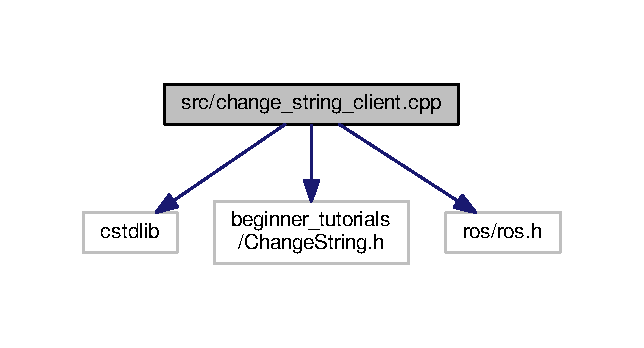
\includegraphics[width=309pt]{change__string__client_8cpp__incl}
\end{center}
\end{figure}
\subsection*{Functions}
\begin{DoxyCompactItemize}
\item 
int \hyperlink{change__string__client_8cpp_a3c04138a5bfe5d72780bb7e82a18e627}{main} (int argc, char $\ast$$\ast$argv)
\end{DoxyCompactItemize}


\subsection{Function Documentation}
\index{change\+\_\+string\+\_\+client.\+cpp@{change\+\_\+string\+\_\+client.\+cpp}!main@{main}}
\index{main@{main}!change\+\_\+string\+\_\+client.\+cpp@{change\+\_\+string\+\_\+client.\+cpp}}
\subsubsection[{\texorpdfstring{main(int argc, char $\ast$$\ast$argv)}{main(int argc, char **argv)}}]{\setlength{\rightskip}{0pt plus 5cm}int main (
\begin{DoxyParamCaption}
\item[{int}]{argc, }
\item[{char $\ast$$\ast$}]{argv}
\end{DoxyParamCaption}
)}\hypertarget{change__string__client_8cpp_a3c04138a5bfe5d72780bb7e82a18e627}{}\label{change__string__client_8cpp_a3c04138a5bfe5d72780bb7e82a18e627}
This is the client node of the service \char`\"{}change\+\_\+string\char`\"{}. One would enter a string argument, which would be sent to the server node. And then, the server node would change its publishing content based on the string provided by the user. If no service is called, then the default string is \char`\"{}\+Hello\char`\"{}. 
\hypertarget{listener_8cpp}{}\section{src/listener.cpp File Reference}
\label{listener_8cpp}\index{src/listener.\+cpp@{src/listener.\+cpp}}
{\ttfamily \#include \char`\"{}ros/ros.\+h\char`\"{}}\\*
{\ttfamily \#include \char`\"{}std\+\_\+msgs/\+String.\+h\char`\"{}}\\*
Include dependency graph for listener.\+cpp\+:\nopagebreak
\begin{figure}[H]
\begin{center}
\leavevmode
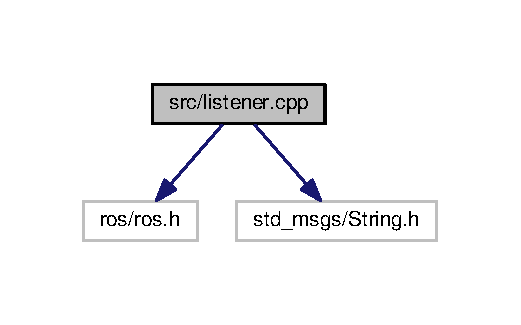
\includegraphics[width=250pt]{listener_8cpp__incl}
\end{center}
\end{figure}
\subsection*{Functions}
\begin{DoxyCompactItemize}
\item 
void \hyperlink{listener_8cpp_ae5c0c11b4a60030ee8df1a3ae0b6f758}{chatter\+Callback} (const std\+\_\+msgs\+::\+String\+::\+Const\+Ptr \&msg)
\item 
int \hyperlink{listener_8cpp_a3c04138a5bfe5d72780bb7e82a18e627}{main} (int argc, char $\ast$$\ast$argv)
\end{DoxyCompactItemize}


\subsection{Function Documentation}
\index{listener.\+cpp@{listener.\+cpp}!chatter\+Callback@{chatter\+Callback}}
\index{chatter\+Callback@{chatter\+Callback}!listener.\+cpp@{listener.\+cpp}}
\subsubsection[{\texorpdfstring{chatter\+Callback(const std\+\_\+msgs\+::\+String\+::\+Const\+Ptr \&msg)}{chatterCallback(const std_msgs::String::ConstPtr &msg)}}]{\setlength{\rightskip}{0pt plus 5cm}void chatter\+Callback (
\begin{DoxyParamCaption}
\item[{const std\+\_\+msgs\+::\+String\+::\+Const\+Ptr \&}]{msg}
\end{DoxyParamCaption}
)}\hypertarget{listener_8cpp_ae5c0c11b4a60030ee8df1a3ae0b6f758}{}\label{listener_8cpp_ae5c0c11b4a60030ee8df1a3ae0b6f758}
In the callback function, the listener node replies what it received from the talker node. If the user didn\textquotesingle{}t modify the original message through change\+\_\+string service, the listener replies with \char`\"{}\+I heard nothing new\char`\"{}. \index{listener.\+cpp@{listener.\+cpp}!main@{main}}
\index{main@{main}!listener.\+cpp@{listener.\+cpp}}
\subsubsection[{\texorpdfstring{main(int argc, char $\ast$$\ast$argv)}{main(int argc, char **argv)}}]{\setlength{\rightskip}{0pt plus 5cm}int main (
\begin{DoxyParamCaption}
\item[{int}]{argc, }
\item[{char $\ast$$\ast$}]{argv}
\end{DoxyParamCaption}
)}\hypertarget{listener_8cpp_a3c04138a5bfe5d72780bb7e82a18e627}{}\label{listener_8cpp_a3c04138a5bfe5d72780bb7e82a18e627}
The ros\+::init() function needs to see argc and argv so that it can perform any R\+OS arguments and name remapping that were provided at the command line. For programmatic remappings you can use a different version of init() which takes remappings directly, but for most command-\/line programs, passing argc and argv is the easiest way to do it. The third argument to init() is the name of the node.

You must call one of the versions of ros\+::init() before using any other part of the R\+OS system.

Node\+Handle is the main access point to communications with the R\+OS system. The first Node\+Handle constructed will fully initialize this node, and the last Node\+Handle destructed will close down the node.

The subscribe() call is how you tell R\+OS that you want to receive messages on a given topic. This invokes a call to the R\+OS master node, which keeps a registry of who is publishing and who is subscribing. Messages are passed to a callback function, here called chatter\+Callback. subscribe() returns a Subscriber object that you must hold on to until you want to unsubscribe. When all copies of the Subscriber object go out of scope, this callback will automatically be unsubscribed from this topic.

The second parameter to the subscribe() function is the size of the message queue. If messages are arriving faster than they are being processed, this is the number of messages that will be buffered up before beginning to throw away the oldest ones.

ros\+::spin() will enter a loop, pumping callbacks. With this version, all callbacks will be called from within this thread (the main one). ros\+::spin() will exit when Ctrl-\/C is pressed, or the node is shutdown by the master.
\hypertarget{passCustStr_8cpp}{}\section{src/pass\+Cust\+Str.cpp File Reference}
\label{passCustStr_8cpp}\index{src/pass\+Cust\+Str.\+cpp@{src/pass\+Cust\+Str.\+cpp}}
{\ttfamily \#include \char`\"{}ros/ros.\+h\char`\"{}}\\*
{\ttfamily \#include \char`\"{}std\+\_\+msgs/\+String.\+h\char`\"{}}\\*
{\ttfamily \#include \char`\"{}beginner\+\_\+tutorials/\+Change\+String.\+h\char`\"{}}\\*
{\ttfamily \#include \char`\"{}pass\+Cust\+Str.\+hpp\char`\"{}}\\*
Include dependency graph for pass\+Cust\+Str.\+cpp\+:
\nopagebreak
\begin{figure}[H]
\begin{center}
\leavevmode
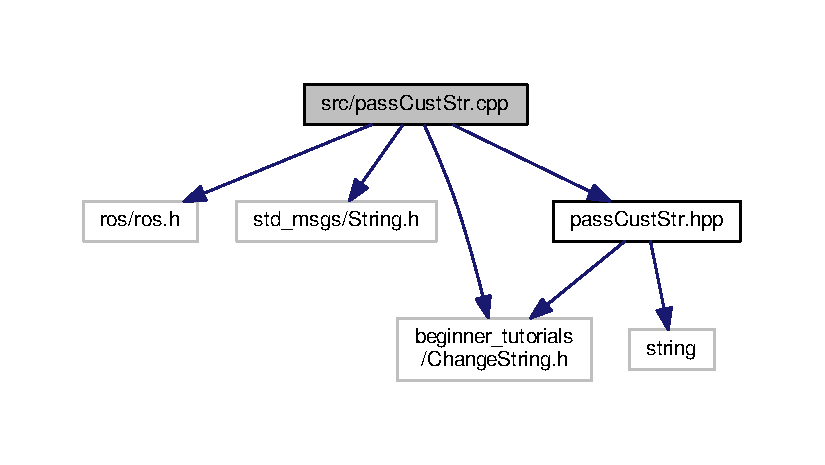
\includegraphics[width=350pt]{passCustStr_8cpp__incl}
\end{center}
\end{figure}


\subsection{Detailed Description}
@ brief A member function of \hyperlink{classpassCustStr}{pass\+Cust\+Str} class that stores the response from the service. 
\hypertarget{talker_8cpp}{}\section{src/talker.cpp File Reference}
\label{talker_8cpp}\index{src/talker.\+cpp@{src/talker.\+cpp}}
{\ttfamily \#include $<$string$>$}\\*
{\ttfamily \#include $<$sstream$>$}\\*
{\ttfamily \#include $<$cstdlib$>$}\\*
{\ttfamily \#include \char`\"{}ros/ros.\+h\char`\"{}}\\*
{\ttfamily \#include \char`\"{}tf/transform\+\_\+broadcaster.\+h\char`\"{}}\\*
{\ttfamily \#include \char`\"{}std\+\_\+msgs/\+String.\+h\char`\"{}}\\*
{\ttfamily \#include \char`\"{}beginner\+\_\+tutorials/\+Change\+String.\+h\char`\"{}}\\*
{\ttfamily \#include \char`\"{}pass\+Cust\+Str.\+hpp\char`\"{}}\\*
Include dependency graph for talker.\+cpp\+:
\nopagebreak
\begin{figure}[H]
\begin{center}
\leavevmode
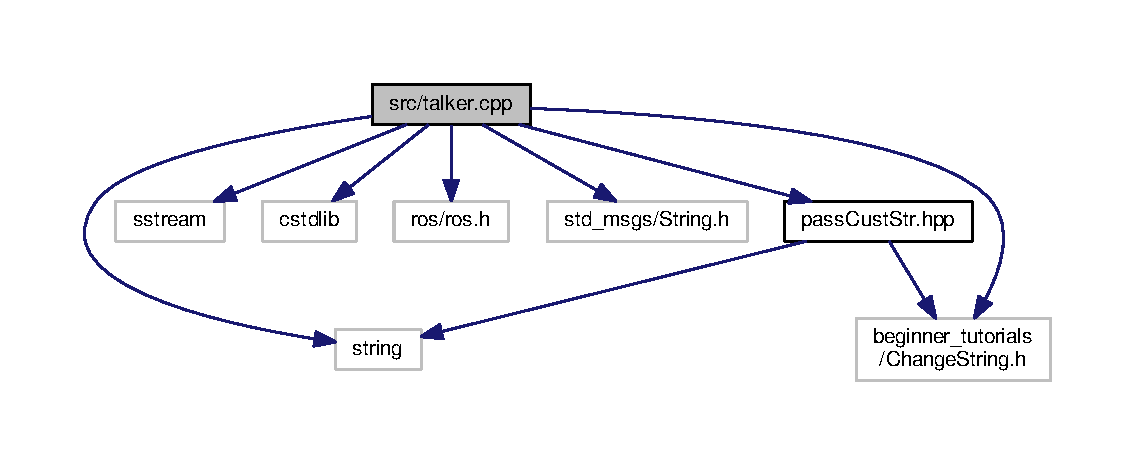
\includegraphics[width=350pt]{talker_8cpp__incl}
\end{center}
\end{figure}
\subsection*{Functions}
\begin{DoxyCompactItemize}
\item 
int \hyperlink{talker_8cpp_a3c04138a5bfe5d72780bb7e82a18e627}{main} (int argc, char $\ast$$\ast$argv)
\end{DoxyCompactItemize}


\subsection{Function Documentation}
\index{talker.\+cpp@{talker.\+cpp}!main@{main}}
\index{main@{main}!talker.\+cpp@{talker.\+cpp}}
\subsubsection[{\texorpdfstring{main(int argc, char $\ast$$\ast$argv)}{main(int argc, char **argv)}}]{\setlength{\rightskip}{0pt plus 5cm}int main (
\begin{DoxyParamCaption}
\item[{int}]{argc, }
\item[{char $\ast$$\ast$}]{argv}
\end{DoxyParamCaption}
)}\hypertarget{talker_8cpp_a3c04138a5bfe5d72780bb7e82a18e627}{}\label{talker_8cpp_a3c04138a5bfe5d72780bb7e82a18e627}
This code is adopted from the R\+OS message tutorial. It has been modified to be able to accept the user-\/defined string and changes its output accordingly. In addition, the code also accepts a frequency argument, which controls the rate of rate publishing. A class type is defined to pass service message as string data type

The ros\+::init() function needs to see argc and argv so that it can perform any R\+OS arguments and name remapping that were provided at the command line. For programmatic remappings you can use a different version of init() which takes remappings directly, but for most command-\/line programs, passing argc and argv is the easiest way to do it. The third argument to init() is the name of the node.

You must call one of the versions of ros\+::init() before using any other part of the R\+OS system.

Node\+Handle is the main access point to communications with the R\+OS system. The first Node\+Handle constructed will fully initialize this node, and the last Node\+Handle destructed will close down the node.

The service function enables the user to change the base string. The R\+OS service consists of two parts, request and reply. The talker is a publishig node and also a server node. The server node will receive a message from the client node when the client is called.

The advertise() function is how you tell R\+OS that you want to publish on a given topic name. This invokes a call to the R\+OS master node, which keeps a registry of who is publishing and who is subscribing. After this advertise() call is made, the master node will notify anyone who is trying to subscribe to this topic name, and they will in turn negotiate a peer-\/to-\/peer connection with this node. advertise() returns a Publisher object which allows you to publish messages on that topic through a call to publish(). Once all copies of the returned Publisher object are destroyed, the topic will be automatically unadvertised.

The second parameter to advertise() is the size of the message queue used for publishing messages. If messages are published more quickly than we can send them, the number here specifies how many messages to buffer up before throwing some away.

This is a message object. You stuff it with data, and then publish it.

The publish() function is how you send messages. The parameter is the message object. The type of this object must agree with the type given as a template parameter to the advertise$<$$>$() call, as was done in the constructor above.
%--- End generated contents ---

% Index
\backmatter
\newpage
\phantomsection
\clearemptydoublepage
\addcontentsline{toc}{chapter}{Index}
\printindex

\end{document}
